\chapter{Почему протекают химические реакции}

\section{Энергия и её виды}

В этой главе мы затронем одну из важнейших тем для понимания самой концепции химических превращений, а именно почему в принципе химические соединения склонны к каким-либо процессам изменения своего состава.

Мы постараемся ответить на два вопроса:

\begin{itemize}
    \item Почему химические реакции принципиально возможны?
    \item Что является движущей силой тех или иных реакций?
\end{itemize}

Для того чтобы сделать это, в этом разделе мы прежде всего разберёмся с понятием энергии, её видами, преобразованием одного вида в другой и тем, как изменяется энергия при химических превращениях веществ.

\term{Энергия}{energy}{энергия}~--- это способность совершать работу. Если мы говорим, что объект обладает высокой энергией, то подразумеваем, что он способен совершить относительно большую работу. И энергия, и работа измеряются в джоулях (\unit{\ruJ}).

Любой объект (или система) обладает так называемой \term{внутренней энергией}{internal_energy}{внутренняя энергия} $U$~--- суммарной энергией всех частиц (молекул, атомов, электронов), из которых состоит тело. Внутренняя энергия не зависит от положения тела и от его движения как целого. Например, летящий и стоящий на аэродроме самолёт при одной температуре обладают одинаковой внутренней энергией.

Внутренняя энергия, так же, как и работа, измеряется в джоулях. Однако поскольку понятие внутренней энергии применяется к веществу, то её часто относят к количеству вещества ($U_m$) и выражают в \unit{\ruJ\per\ruMole}. Абсолютные значения внутренней энергии неизвестны (потому что нельзя точно подсчитать все виды энергии всех частиц), но мы можем работать с величинами \emph{изменения внутренней энергии} $\Delta U$.

\subsection*{Первое начало термодинамики}

Энергия не может появиться из ниоткуда и исчезнуть в никуда, она может только превратиться из одного вида в другой. Другими словами, энергию нельзя ни создать, ни уничтожить. Её можно только передать от одной системы к другой или преобразовать из одного вида в другой.

Например, когда горит костёр, мы не создаём энергию, а преобразуем химическую энергию, запасённую в древесине, в энергию излучения и теплоту. При этом сама энергия в древесине тоже не появилась из ниоткуда, а накопилась в результате преобразования энергии солнечного излучения в химическую энергию (рис.~\ref{fig:energy_conservation}).

\begin{figure}[htbp]
    \centering
    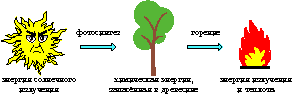
\includegraphics[width=11cm]{figs/energy_and_its_forms/energy_conservation.pdf}
    \caption{Энергия преобразуется из одних видов в другие, но всегда сохраняется.}
    \label{fig:energy_conservation}
\end{figure}

Описанный принцип по своей сути~--- это закон сохранения энергии, для которого существует великое множество формулировок. Нас же будет интересовать его применение в области химических превращений, где его формулируют как \term{первое начало термодинамики}{first_law_of_thermodynamics}{первое начало термодинамики}\footnote{Термодинамика~--- это раздел физики, изучающий превращение энергии из одной формы в другую, связь между энергией и теплотой, а также доступность энергии для совершения работы.}: \emph{внутренняя энергия изолированной системы постоянна}.

Поясним, что имеется в виду. В качестве системы представьте себе объект, который мы рассматриваем (например, определённые количества веществ, в том числе реагирующие друг с другом). Всё, что находится вокруг системы~--- это окружение. Изолированная систе\-ма~--- это система, которая не обменивается с окружением ни веществом, ни энергией.

Обмениваться энергией с окружением объект может двумя способами~--- совершая работу (например, расширяясь) или передавая теплоту. При этом теплота и работа~--- это именно \emph{способы передачи энергии}, а не её запасы внутри объекта. Например, некорректно говорить, что в стакане воды <<столько-то джоулей теплоты>>. Теплота возникает только тогда, когда энергия переходит от одного тела к другому (или, в нашем случае, между системой и окружением). Поэтому изменить внутреннюю энергию системы можно, передавая или забирая у неё теплоту $Q$, либо совершая над телом работу $W$:

\begin{equation}
    \label{eq:first_law_of_thermodynamics}
    \boxed{\Delta U = Q + W}.
\end{equation}

Выражение~\eqref{eq:first_law_of_thermodynamics} представляет собой математическую запись первого начала термодинамики. Если система изолирована, то внутренняя энергия не может измениться, потому что ей неоткуда взяться и некуда уйти, если передача теплоты и совершение работы невозможны.

Рассмотрим по очереди виды энергии, которые понадобятся нам в дальнейшем. Наиболее важны следующие три вида энергии:

\begin{itemize}
    \item кинетическая;
    \item потенциальная гравитационная;
    \item потенциальная химическая.
\end{itemize}

\subsection*{Кинетическая энергия}

Это энергия, которая связана с движением объекта как целого и зависит от его массы и скорости:

\begin{equation*}
    E = \frac{m{\upsilon}^2}{2}.
\end{equation*}

Чем массивнее объект и чем быстрее он движется, тем большей кинетической энергией он обладает, причём энергия пропорциональна \emph{квадрату скорости}\footnote{Именно в этом заключается опасность превышения скорости при движении на автомобиле: при увеличении скорости вдвое тормозной путь возрастает вчетверо, делая движение значительно более опасным.}.

Применительно к веществу мы можем говорить о кинетической энергии поступательного движения отдельных молекул. При этом она напрямую зависит от температуры вещества~--- в одном и том же веществе при более низкой температуре молекулы движутся медленнее, чем при более высокой.

К примеру, в жидкости с ростом температуры всё больше молекул набирает энергию, достаточную, чтобы преодолеть межмолекулярные силы и покинуть её,~--- из-за этого над жидкостью растёт давление насыщенного пара. Когда давление пара сравнивается с внешним давлением, начинается \emph{кипение}: пузырьки пара получают возможность образовываться прямо в толще жидкости, а не только на её поверхности.

Отдельно нужно сказать про связь кинетической энергии частиц вещества и его агрегатного состояния. Вопреки распространённому заблуждению, кинетическая энергия частиц вещества \emph{не зависит} от его агрегатного состояния. Агрегатное состояние определяется \emph{балансом} между кинетической энергией (которая <<расталкивает>> частицы) и потенциальной энергией (которую мы сейчас изучим) межмолекулярного взаимодействия, которая удерживает их вместе. При фазовом переходе кинетическая энергия не меняется, а изменяется именно потенциальная.

\subsection*{Потенциальная гравитационная энергия}

Потенциальной называют энергию, каким-либо образом запасённую в объекте и готовую к преобразованию в другой вид энергии при наступлении некоторых событий.

\term{Потенциальной гравитационной энергией}{gravitational_potential_energy}{потенц. гравит. энергия} называется энергия, которой объект обладает из-за своего относительного положения в гравитационном поле.

Рассмотрим мяч, который ребёнок выбрасывает из окна дома (рис.~\ref{fig:potential_and_kinetic_energy}, сопротивлением воздуха пренебрегаем). В верхней точке (пока ребёнок не отпустил мяч) он не двигается, но мы знаем, что если его отпустить, то он полетит вниз, набирая скорость, то есть увеличивая свою кинетическую энергию.

Другими словами, в верхней точке мяч обладал запасом потенциальной энергии, которая при его движении в поле земного тяготения начала преобразовываться в кинетическую энергию. У самой земли кинетическая энергия мяча максимальна (вся потенциальная энергия уже преобразовалась за время его движения), а потенциальная минимальна (её удобно принять за ноль), потому что, несмотря на то что мяч остаётся в поле тяготения, ниже уровня земли он опуститься не может.

\begin{figure}[htbp]
    \centering
    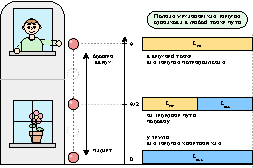
\includegraphics[width=12cm]{figs/energy_and_its_forms/potential_and_kinetic_energy.pdf}
    \caption{Превращение потенциальной энергии в кинетическую.}
    \label{fig:potential_and_kinetic_energy}
\end{figure}

Потенциальная и кинетическая энергии могут обратимо превращаться друг в друга. Если подбросить мяч с уровня земли вверх, то он будет замедляться, пока не остановится; при этом кинетическая энергия его движения будет превращаться в потенциальную. В любой точке его движения полная механическая энергия системы (кинетическая + потенциальная) остаётся одинаковой.

\term{Полной энергией системы}{total_system_energy}{полная энергия системы} называют сумму её внутренней энергии, кинетической энергии и потенциальной энергии системы как целого.

\subsection*{Потенциальная химическая энергия}

Потенциальная химическая энергия обусловлена тем, что связь обладает <<прочностью>> и для того, чтобы разорвать её, нужно приложить энергию (например, нагреть вещество). Исходные атомы до образования химической связи имели более высокую потенциальную энергию, но при образовании связи потенциальная энергия системы электронов и ядер снизилась (рис.~\ref{fig:chemical_potential_energy}). При этом в ходе образования связи разность потенциальных энергий исходных и связанных атомов преобразуется в другие виды энергии.

\begin{figure}[htbp]
    \centering
    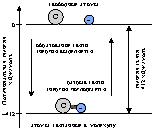
\includegraphics[width=7.5cm]{figs/energy_and_its_forms/chemical_potential_energy.pdf}
    \caption{Понижение потенциальной энергии системы при образовании химической связи.}
    \label{fig:chemical_potential_energy}
\end{figure}

Получается, что в этом случае величина потенциальной энергии отрицательна (если принять за ноль потенциальную энергию разделённых исходных атомов). Для проведения расчётов это не имеет значения, так же как и для внутренней энергии, поскольку нам важны не абсолютные значения, а разность между рассматриваемыми уровнями.

Таким образом, при образовании связи выделяется энергия, а при разрыве~--- поглощается.

Количество энергии, необходимое для разрыва химической связи, называют \emph{энергией связи}. Поскольку для одной связи это весьма малая величина, её относят к 1~молю связей и выражают в \unit{\ruKJ\per\ruMole}.

Например, энергия связи \ce{C\bond{1}H} составляет примерно \qty{412}{\ruKJ\per\ruMole}, а \ce{N\bond{1}H}~--- \qty{390}{\ruKJ\per\ruMole}.

Энергия связи зависит от:

\begin{itemize}
    \item того, какие атомы связаны. Например, одинарная связь между атомами углерода слабее, чем между атомами углерода и водорода ($E_{\ce{C\bond{1}C}} \approx$ \num{346}--\qty{348}{\ruKJ\per\ruMole}, $E_{\ce{C\bond{1}H}} \approx \qty{412}{\ruKJ\per\ruMole}$);
    \item того, с какими другими атомами связаны атомы, образующие связь. Например, энергия связи \ce{H\bond{1}O} выше в молекуле воды ($\approx \qty{464}{\ruKJ\per\ruMole}$), чем в молекуле пероксида водорода ($\approx \qty{365}{\ruKJ\per\ruMole}$)\footnote{При этом, хотя энергия одной и той же связи различается в зависимости от окружения, она будет в целом близка к определённому значению, которое называют \emph{средней энергией связи}.}.
\end{itemize}

Внимательный читатель может задать резонный вопрос: если энергия при образовании химической связи из атомов всегда выделяется, а потенциальная энергия системы при этом снижается, то о каких таких <<запасах>> химической энергии мы говорим? Дело в том, что, когда происходит накопление химической энергии, ранее существовавшие химические связи разрываются, а вместо них образуются новые, но суммарно более слабые (с меньшими энергиями). Так, например, при фотосинтезе (по сути~--- запасании энергии Солнца в виде химической энергии) углекислый газ и вода превращаются в углеводы и кислород. Суммарная энергия связей в продуктах фотосинтеза меньше, чем в исходных веществах, поэтому потенциальная энергия системы возрастает. Обратное преобразование (с выделением энергии) будет происходить в живых организмах, когда углеводы в процессе клеточного дыхания окисляются до менее энергоёмких молекул углекислого газа и воды.

\begin{termlist}
    \hyperref[term:energy]{Энергия},
    \hyperref[term:internal_energy]{внутренняя энергия},
    \hyperref[term:first_law_of_thermodynamics]{первое начало термодинамики},
    \hyperref[term:gravitational_potential_energy]{потенциальная гравитационная энергия},
    \hyperref[term:total_system_energy]{полная энергия системы}.
\end{termlist}

\begin{problem}{}{energy_and_its_forms1}
    В теплоизолированном сосуде находится вода. В воду погружена мешалка. Мешалку начинают вращать, и через некоторое время вода нагревается на несколько градусов. Откуда же взялась теплота, ведь термос считается моделью изолированной системы? Не противоречит ли это первому началу термодинамики?
    \begin{sol}{\ref{prob:energy_and_its_forms1}}
        К системе подводится энергия путём совершения работы, поэтому систему нельзя считать изолированной. Механическая работа, совершаемая мешалкой, за счёт сил вязкого трения переходит во внутреннюю энергию воды, вызывая её нагревание. Это полностью подтверждает первое начало термодинамики.

        Обратите внимание, что многое зависит от того, где мы располагаем границу системы. Если включить в систему не только воду, но и привод мешалки, и человека, крутящего её, то она формально станет почти изолированной, и её полная энергия не изменится. В этом случае химическая энергия в человеке перейдёт во внутреннюю энергию воды.
    \end{sol}
\end{problem}

\begin{problem}{}{energy_and_its_forms2}
    Энергия связи \ce{O\bond{1}H} в воде составляет примерно \qty{464}{\ruKJ\per\ruMole}. На какую высоту нужно поднять \qty{1}{\ruMole} воды, чтобы её потенциальная гравитационная энергия оказалась равна энергии всех связей \ce{O\bond{1}H} в этой порции? Ускорение свободного падения \qty{9,8}{\ruM\per\ruS\squared}. Радиус Земли равен \qty{6400}{\ruKm}, сравните с ним полученное значение и объясните, почему это лишь оценка снизу.
    \begin{sol}{\ref{prob:energy_and_its_forms2}}
        В молекуле воды имеется сразу две связи \ce{O\bond{1}H}, значит, в одном моле воды содержится два моля связей с общей энергией $2 \cdot 464 = \qty{928}{\ruKJ}$.

        Масса моля воды $m = \qty{18}{\ruG} = \qty{0,018}{\ruKg}$, потенциальная гравитационная энергия определяется соотношением $E = mgh$, откуда

        \begin{equation*}
            h = \frac{E}{mg} = \frac{\num{928000}}{\num{0,018} \cdot \num{9,8}} \approx \qty{5,3e6}{\ruM} = \qty{5300}{\ruKm}.
        \end{equation*}

        Это составляет более \qty{80}{\percent} радиуса Земли, на таких расстояниях величина ускорения свободного падения уже примерно в три раза меньше, чем у поверхности планеты, так что оценка сильно занижена.
    \end{sol}
\end{problem}

\begin{problem}{}{energy_and_its_forms3}
    Вода кипит при температуре \qty{100}{\degreeCelsius} при нормальном атмосферном давлении. При этом в результате нагрева продолжает подводиться энергия, но температура воды и образующегося пара не растёт. Куда уходит подводимая энергия, учитывая, что пар занимает намного больший объём, чем жидкость, из которой он образовался. Теплота испарения воды составляет \qty{40,7}{\ruKJ\per\ruMole}. Сравните эту величину с энергией связи \ce{O\bond{1}H} в воде (\qty{464}{\ruKJ\per\ruMole}) и объясните, почему они различаются так сильно.
    \begin{sol}{\ref{prob:energy_and_its_forms3}}
        Температура является мерой кинетической энергии движения молекул. Раз она не меняется, кинетическая энергия тоже не меняется, а значит подводимая энергия расходуется на что-то ещё.

        На самом деле большая её часть идёт на увеличение \emph{потенциальной} энергии межмолекулярного взаимодействия. На деле это выглядит как расталкивание молекул на расстояния, на которых они почти не притягиваются друг к другу.

        Также часть энергии тратится на работу расширения. 1~моль пара при \qty{100}{\degreeCelsius} занимает примерно \qty{30}{\ruL}, а моль жидкой воды~--- всего \qty{18}{\ruMl}, то есть объём вырастает примерно в \num{1700} раз. Расширяясь, пар совершает работу над атмосферой, равную $p \Delta V \approx \qty{3,1}{\ruKJ}$. В соответствии с первым началом (там $W$~--- это работа \emph{над} системой) $Q = \qty{40,7}{\ruKJ}$, $W = \qty{-3,1}{\ruKJ}$, так что внутренняя энергия растёт не на все \num{40,7}, а на $\Delta U \approx \qty{37,6}{\ruKJ}$. На работу расширения уходит примерно \qty{8}{\percent} подводимой энергии, а остальное~--- на разрыв межмолекулярных связей.

        Чтобы разложить \qty{1}{\ruMole} воды на атомы, нужно разорвать два моля связей \ce{O\bond{1}H}, то есть затратить около \qty{928}{\ruKJ}, что в двадцать с лишним раз больше, чем на испарение. Причина в том, что при кипении не разрываются очень прочные ковалентные связи, а только водородные связи между молекулами, а они более чем на порядок слабее ковалентных (около \qty{20}{\ruKJ\per\ruMole}).
    \end{sol}
\end{problem}

\begin{problem}{}{energy_and_its_forms4}
    Какие из приведённых утверждений неверны и почему?
    \begin{enumerate}[label=\arabic*)]
        \item В горячей воде больше теплоты, чем в холодной.
        \item Внутренняя энергия стакана воды уменьшилась на \qty{500}{\ruJ}.
        \item В сжатой пружине запасена работа.
        \item Система получила \qty{200}{\ruJ} теплоты и совершила работу \qty{50}{\ruJ}.
    \end{enumerate}
    \begin{sol}{\ref{prob:energy_and_its_forms4}}
        Неверны утверждения 1 и 3. Теплота и работа~--- это \emph{способы передачи} энергии, запасти их нельзя. Правильно было бы сказать так: в горячей воде \emph{внутренняя энергия} больше, чем в холодной при той же массе; в сжатой пружине запасена \emph{потенциальная энергия}.
    \end{sol}
\end{problem}

\begin{problem}{}{energy_and_its_forms5}
    В некоторых учебниках биологии можно встретить фразу <<энергия запасена в макроэргических связях АТФ и выделяется при их разрыве>>. Объясните, в чём неграмотность этой фразы, и предложите правильную формулировку.
    \begin{sol}{\ref{prob:energy_and_its_forms5}}
        Сама по себе химическая связь не содержит запасённой энергии, которая высвобождалась бы при её разрыве. Наоборот, разрыв любой химической связи \emph{всегда} требует затрат энергии. Если бы разрыв связи выделял энергию, молекулы распадались бы самопроизвольно.

        При гидролизе АТФ энергия выделяется не из-за самого факта разрыва связи, а в результате \emph{перегруппировки} связей: на разрыв связей в молекулах АТФ и воды энергии тратится меньше, чем выделяется при образовании новых связей в молекулах АДФ и фосфата (а также при их гидратации).

        \textbf{Правильная формулировка:} \textit{Энергия выделяется в ходе реакции гидролиза АТФ, так как суммарная энергия продуктов реакции (с учётом образования новых химических связей и гидратации) ниже, чем у исходных реагентов}.
    \end{sol}
\end{problem}

\clearpage

\section{Как передаётся энергия}

Разберём более подробно, что мы называем системой и окружением. Объект или набор объектов, который мы рассматриваем, когда ведём разговор про энергетические процессы (человеческая мышца, автомобиль, горячая чашка на столе), и у которого определены границы (то есть мы можем чётко выделить его), называется \term{системой}{thermodynamic_system}{термодинамическая система}. Границы при этом могут быть реальными или воображаемыми (рис.~\ref{fig:night_city}).

\begin{figure}[htbp]
    \centering
    
\includegraphics[width=5cm]{figs/how_is_energy_transferred/night_city.pdf}
    \caption{Пример воображаемой границы системы: кубический километр атмосферы над городом для оценки остывания ночью.}
    \label{fig:night_city}
\end{figure}

Всё, что находится вокруг системы, называют \term{окружением}{thermodynamic_environment}{термодинамическое окружение}. Для приведённых выше примеров систем окружением можно считать, например, ткани организма вокруг мышцы, воздух вокруг автомобиля и чашки, а также стол под чашкой.

Не воспринимайте это так, словно для любых объектов система и окружение заранее определены, мы сами выбираем их в зависимости от того, что хотим рассмотреть. Система может состоять из нескольких тел, кроме того, мы можем вообще не выделять окружение, если оно нам не нужно (например, если мы рассматриваем два заряда (рис.~\ref{fig:charges_at_distance_r_attract}) на некотором расстоянии друг от друга).

\begin{figure}[htbp]
    \centering
    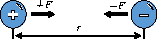
\includegraphics[width=6cm]{figs/how_is_energy_transferred/charges_at_distance_r_attract.pdf}
    \caption{Разноимённые заряды на расстоянии $r$~--- пример системы, для которой окружение можно не выделять.}
    \label{fig:charges_at_distance_r_attract}
\end{figure}

В зависимости от того, что может происходить с системой и окружением, различают три вида систем (рис.~\ref{fig:types_of_systems}):

\begin{itemize}
    \item \term{Открытая система}{open_system}{открытая система}~--- может обмениваться с окружением и энергией и веществом. К примеру, чашка на столе~--- это открытая система~--- она отдаёт тепло в окружающее пространство и одновременно содержимое чашки испаряется, при этом происходит перенос вещества в окружение.
    \item \term{Закрытая система}{closed_system}{закрытая система}~--- может обмениваться с окружением энергией, но не может веществом. Это произойдёт, если мы накроем чашку крышкой.
    \item \term{Изолированная система}{isolated_system}{изолированная система}~--- не может обмениваться с окружением ни веществом, ни энергией. Бытовым приближённым примером такой системы является закрытый термос. Строго изолированных систем не существует, поэтому даже самый прекрасно сделанный термос со временем остывает.
\end{itemize}

\begin{figure}[htbp]
    \centering
    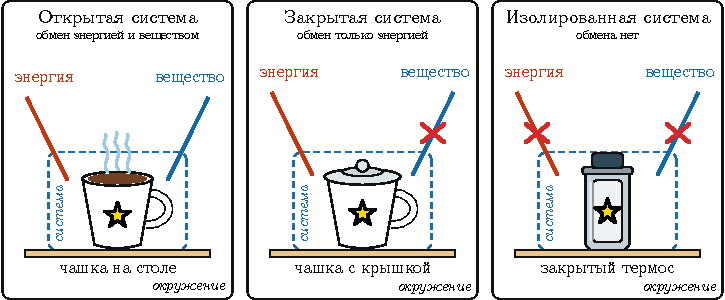
\includegraphics[width=\linewidth]{figs/how_is_energy_transferred/types_of_systems.pdf}
    \caption{Типы термодинамических систем.}
    \label{fig:types_of_systems}
\end{figure}

Поскольку энергию нельзя создать или уничтожить, она может лишь передаваться между системой и окружением. Первый закон термодинамики говорит нам о том, что для закрытой системы её внутреннюю энергию можно изменить только двумя путями: совершая \emph{работу над системой} (или наоборот, путём совершения системой работы) и путём \emph{теплопередачи}. При этом суммарная энергия системы и окружения останется той же самой, просто произойдёт перераспределение энергии. Для открытых систем доступен и третий путь~--- физически перенести вещество между системой и окружением (рис.~\ref{fig:first_law_of_thermodynamics}).

\begin{figure}[htbp]
    \centering
    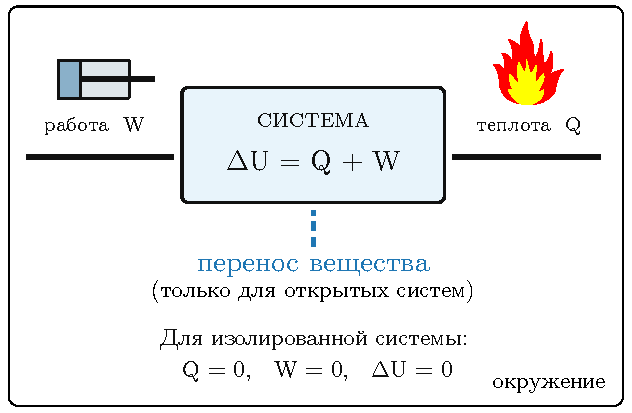
\includegraphics[width=8cm]{figs/how_is_energy_transferred/first_law_of_thermodynamics.pdf}
    \caption{Три способа изменить внутреннюю энергию системы.}
    \label{fig:first_law_of_thermodynamics}
\end{figure}

\subsection*{Передача энергии в виде работы}

\term{Работа}{work}{работа}~--- это энергия, которую сила передаёт телу при его перемещении. Рассмотрим камень, который человек поднимает с земли. Камень, находящийся в поле действия силы тяготения~--- это окружение, а человек~--- это система. Химическая энергия, накопленная человеком в виде питательных веществ, преобразуется в кинетическую энергию его движения, которая передаётся камню (то есть от системы к окружению), совершая над ним работу. Кинетическая энергия системы расходуется на увеличение потенциальной энергии камня\footnote{Если говорить точнее, то вначале камню передаётся кинетическая энергия, которая уже затем при подъёме против силы тяжести превращается в потенциальную энергию.}.

При этом система совершает работу над окружением, причём чем больше энергии передаст система окружению, тем выше будет поднят камень и тем большая работа будет совершена (рис.~\ref{fig:work_lifting_stone}).

\begin{figure}[htbp]
    \centering
    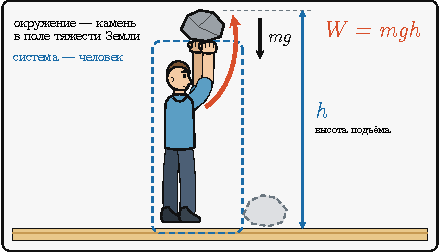
\includegraphics[width=10cm]{figs/how_is_energy_transferred/work_lifting_stone.pdf}
    \caption{Работа, осуществляемая при перемещении объекта.}
    \label{fig:work_lifting_stone}
\end{figure}

Количество работы можно подсчитать, умножив приложенную силу на пройденное объектом расстояние:

\begin{equation*}
    W = F d \cos\alpha,
\end{equation*}

где $W$~--- совершённая над телом работа, Дж; $F$~--- приложенная сила (ньютон, Н); $d$~--- расстояние, м, $\alpha$~--- угол между приложенной силой и направлением перемещения.

Описанный выше тип работы называется \emph{механической работой}. Однако химические реакции чаще всего совершают работу других видов (прежде всего работу расширения). Запомните, что общий принцип для всех них будет один и тот же:

\begin{equation}
    \label{eq:general_work_formula}
    \text{Работа} = \text{обобщённая сила} \cdot \text{изменение обобщённой координаты}.
\end{equation}

Что же это за другие виды работы, которые может осуществлять химическая реакция? В общем и целом работу, совершаемую химической реакцией, делят на \emph{работу расширения} (которая совершается сама по себе, когда объём реагирующей системы изменяется) и \emph{полезную работу}, для осуществления которой необходим \emph{механизм сопряжения} (например, электроды и внешняя цепь, фермент, мембрана, белковый мотор). Работу расширения мы детально рассмотрим далее, а виды полезной работы приведём в таблице~\ref{tab:types_of_work} без детального описания каждого типа. Обратите внимание, что каждый тип работы соответствует общей формуле~\eqref{eq:general_work_formula}.

\begin{table}[htbp]
    \small
    \caption{Виды полезной работы, которую может совершать химическая реакция. $A'$~--- работа, совершаемая системой; $\varphi$~--- электрический потенциал, $q$~--- заряд; $\mu$~--- химический потенциал, $n$~--- количество вещества; $\sigma$~--- поверхностное натяжение, $A_{\text{пов}}$~--- площадь поверхности; $F$~--- сила, $x$~--- перемещение; $f$~--- сила растяжения, $l$~--- длина.}
    \label{tab:types_of_work}
    \begin{tabularx}{\textwidth}{
        >{\hsize=1\hsize}Y
        >{\hsize=0.8\hsize}Y
        >{\hsize=1.2\hsize}Y
        }
        \hline
        \rowcolor{green!5}
        Вид работы & Формула & Где встречается \\
        \hline
        Электрическая & $A' = \Delta\varphi \cdot \Delta q$ & Гальванический элемент, топливный элемент, аккумулятор, электролиз (работа внешних сил) \\
        \hline
        Перенос вещества против градиента (химическая) & $A' = \Delta\mu \cdot \Delta n$ & В биохимии: \ce{Na+}/\ce{K+}-АТФаза, протонные насосы; сопряжение с гидролизом АТФ \\
        \hline
        Электрохимическая (объединяет две предыдущие) & $A' = \Delta\mu \cdot \Delta n + \Delta\varphi \cdot \Delta q$ & Дыхательная цепь митохондрий, хемиосмос \\
        \hline
        Поверхностная & $A' = \sigma \Delta A_{\text{пов}}$ & Зародышеобразование, диспергирование, работа ПАВ, пены и эмульсии \\
        \hline
        Механическая (не расширение) & $A' = F \Delta x$ & Мышечное сокращение (актин-миозиновый мотор), жгутик бактерии \\
        \hline
        Деформация, удлинение & $A' = f \Delta l$ & Сокращающиеся полимеры, коллаген, pH-чувствительные гели \\
        \hline
    \end{tabularx}
\end{table}

\subsection*{Передача энергии в виде теплоты}

Второй способ передачи энергии~--- это \term{теплота}{heat}{теплота}. Теплота в бытовом смысле~--- это то, как человек ощущает высокую температуру объектов, однако это не совсем правильное восприятие понятия теплоты, потому что на самом деле теплота~--- это \emph{способ передачи энергии от горячего тела к холодному}, а не вещь сама по себе. Именно поэтому теплота имеет ту же размерность, что и энергия~--- Джоули, а смысл количества теплоты в том, сколько энергии было передано.

Если объект получает энергию в виде теплоты, то он нагревается\footnote{Исключение составляют фазовые переходы, например, плавление льда, при которых энергия передаётся, но температура остаётся одной и той же пока не завершится фазовый переход.}, если отдаёт~--- то охлаждается.

Передача энергии в виде теплоты происходит всегда \emph{самопроизвольно} (то есть не нужно совершать какие-либо действия для запуска и поддержания этого процесса) и продолжается до тех пор, пока температуры системы и окружения не сравняются.

Необходимо чётко понимать различие между теплотой и \term{температурой}{temperature}{температура}. Температура определяет \emph{направление} самопроизвольной теплопередачи.

Температура объекта определяется, в первую очередь, кинетической энергией частиц, из которых состоит система (рис.~\ref{fig:temperature_particles}). Атомы и молекулы вещества находятся в постоянном движении и чем более интенсивно они движутся, тем больше способность передавать энергию и тем выше его температура.

\begin{figure}[htbp]
    \centering
    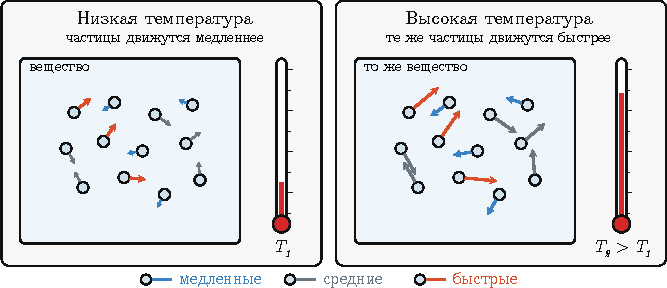
\includegraphics[width=\linewidth]{figs/how_is_energy_transferred/temperature_particles.pdf}
    \caption{При любой температуре в веществе имеются как относительно медленно, так и быстро движущиеся частицы.}
    \label{fig:temperature_particles}
\end{figure}

Однако не все частицы имеют одинаковые энергии: в веществе имеются как частицы с более высокими энергиями, так и с более низкими. Когда мы говорим о температуре, мы подразумеваем некоторую среднюю энергию всех частиц вещества.

Температура показывает не общий запас тепловой энергии, а именно способность передавать её более холодным объектам. Например, в ведре холодной воды запасено больше внутренней энергии, чем в раскалённой скрепке, но передача тепловой энергии может происходить только от скрепки к воде, а не наоборот.

Давайте рассмотрим распределение количества молекул газа в зависимости от их энергии (рис.~\ref{fig:kinetic_energy_distribution})~--- так называемое \term{распределение Максвелла~--- Больцмана}{Maxwell-Boltzmann_distribution}{распр. Максвелла~---Больцмана}.

\begin{figure}[htbp]
    \centering
    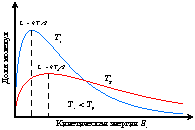
\includegraphics[width=8cm]{figs/how_is_energy_transferred/kinetic_energy_distribution.pdf}
    \caption{Распределение Максвелла~--- Больцмана при двух температурах.}
    \label{fig:kinetic_energy_distribution}
\end{figure}

Вид распределения меняется в зависимости от температуры вещества $T$, при этом при более высоких значениях $T$ количество молекул с высокой кинетической энергией увеличивается, а распределение становится более пологим. То есть при переходе от $T_1$ к $T_2$ кривая не просто поднимается, а \emph{перестраивается}: максимум смещается вправо и одновременно понижается, а распределение становится шире. Обратите внимание, что даже при высоких значениях температуры имеются как молекулы с относительно высокой, так и с относительно низкой энергией.

Наибольшее количество молекул при данной температуре $T$ имеет энергию $E = \frac{kT}{2}$\footnote{$k$~--- постоянная Больцмана, \qty{1,380649e-23}{\ruJ\per\ruK}.}~--- это максимумы приведённых кривых.

Говорить о температуре объектов на уровне атомов не имеет смысла, поскольку температура подразумевает распределение частиц по энергиям, а измерить температуру отдельно взятой микрочастицы невозможно, для неё необходимо использовать понятие <<энергия частицы>>.

\begin{termlist}
    \hyperref[term:thermodynamic_system]{Термодинамическая система},
    \hyperref[term:thermodynamic_environment]{термодинамическое окружение},
    \hyperref[term:open_system]{открытая система},
    \hyperref[term:closed_system]{закрытая система},
    \hyperref[term:isolated_system]{изолированная система},
    \hyperref[term:work]{работа},
    \hyperref[term:heat]{теплота},
    \hyperref[term:temperature]{температура},
    \hyperref[term:Maxwell-Boltzmann_distribution]{распределение Максвелла~--- Больцмана}.
\end{termlist}

\begin{problem}{}{how_is_energy_transferred1}
    Максимум кривых, представленных на рис.~\ref{fig:kinetic_energy_distribution}, отвечает \emph{наиболее вероятной} энергии поступательного движения молекул. Как вы считаете, равна ли она \emph{средней} энергии молекул, и, если нет, то больше она или меньше?
    \begin{sol}{\ref{prob:how_is_energy_transferred1}}
        Кривые асимметричны~--- в правой части они значительно дальше удалены от максимума, поэтому среднее арифметическое (средняя энергия молекул) будет больше, чем наиболее вероятная энергия. Если математически проанализировать распределение Максвелла~--- Больцмана, то она окажется ровно втрое больше.
    \end{sol}
\end{problem}

\begin{problem}{}{how_is_energy_transferred2}
    Почему нельзя измерить температуру отдельной молекулы?
    \begin{sol}{\ref{prob:how_is_energy_transferred2}}
        Температура~--- статистическая величина, для одной частицы она попросту не может быть определена. Кроме того, измерение всегда проводится при помощи объекта сравнения, у которого показатель, зависящий от измеряемого, известен. Например, термометр нагревается до температуры измеряемого образца теплопередачей от него, из-за чего изменяется какой-либо показатель веществ внутри термометра, зависящий от температуры (удельный объём жидкости, ЭДС, удлинение металла). В случае отдельной молекулы невозможно создать такой сенсор, который бы сравнялся по энергии с исследуемой молекулой.
    \end{sol}
\end{problem}

\begin{problem}{}{how_is_energy_transferred3}
    Вам необходимо поднять бетонную плиту массой \qty{500}{\ruKg} на высоту \qty{5}{\ruM}. Сколько энергии вам необходимо потратить на осуществление этой работы? Сколько сахара вам необходимо съесть, чтобы компенсировать эти затраты (при сжигании \qty{1}{\ruG} сахарозы в организме выделяется примерно \qty{16,5}{\ruKJ} энергии)?
    \begin{sol}{\ref{prob:how_is_energy_transferred3}}
        $W = Fd\cos\alpha$, где работа совершается против сил тяжести, сила постоянна и направлена вдоль перемещения ($\cos\alpha = 1$), поэтому $W = mgd = 500 \cdot \num{9,8} \cdot 5 = \qty{24500}{\ruJ} = \qty{24,5}{\ruKJ}$. Чтобы компенсировать эту энергию, необходимо $\frac{\num{24,5}}{\num{16,5}} \approx \qty{1,5}{\ruG}$ сахара (треть чайной ложки). Это даёт некоторое представление о том, как велика может быть запасённая химическая энергия и как трудно переработать полученную с пищей энергию посредством физических упражнений. Впрочем, этот расчёт идеализирован, поскольку КПД мышцы примерно \num{20}--\qty{25}{\percent}, поэтому сахара требуется больше~--- около \num{6}--\qty{7,5}{\ruG}.
    \end{sol}
\end{problem}

\begin{problem}{}{how_is_energy_transferred4}
    Подумайте, к какому типу (открытая, закрытая или изолированная) относятся следующие системы:

    \begin{enumerate}[label=\arabic*)]
        \item наша планета;
        \item закрытый термос с горячим чаем;
        \item клетка бактерии;
        \item запаянная ампула с реакционной смесью, находящаяся в водяном термостате;
        \item Вселенная.
    \end{enumerate}

    Есть ли среди них по-настоящему изолированная?
    \begin{sol}{\ref{prob:how_is_energy_transferred4}}
        1)~Обмен веществом между Землёй и окружающим космосом пренебрежимо мал, поскольку масса падающих на неё метеоритов и утечка газов из верхних слоёв атмосферы ничтожны по сравнению со всей массой планеты. Поэтому можно считать, что это \emph{закрытая} система. С другой стороны, планета постоянно обменивается энергией, поглощая излучение Солнца и излучая энергию обратно в космос. Именно проходящий сквозь планету поток энергии делает возможной жизнь.

        2)~Термос можно условно считать \emph{закрытой} системой. На первый взгляд это вроде бы изолированная система, но так можно считать только в течение короткого времени (вы же помните, что чай в термосе всё-таки остывает за несколько часов).

        3)~Клетка~--- это \emph{открытая} система. Через мембрану идёт и вещество, и энергия.

        4)~Ампула является \emph{закрытой} системой: вещество не может пройти сквозь стенки, а энергией она обменивается с термостатом, который и задаёт ей температуру.

        5)~Скорее всего, Вселенная~--- \emph{изолированная} система, ведь обмениваться Вселенной не с чем.
    \end{sol}
\end{problem}

\begin{problem}{}{how_is_energy_transferred5}
    $\bigstar$ В стакан с \qty{250}{\ruG} воды при \qty{20}{\degreeCelsius} опущен электрический кипятильник. За некоторое время воде было передано \qty{50}{\ruKJ} энергии.

    \begin{enumerate}[label=\arabic*)]
        \item Допустим, что система~--- это только вода. Как ей передана энергия~--- в виде теплоты или работы?
        \item Теперь допустим, что система~--- это вода уже вместе с кипятильником, а граница этой системы~--- в месте входа проводов в спираль. Каким способом энергия передана теперь?
        \item Изменилось ли что-нибудь для воды из-за того, что граница проведена по-разному? На сколько градусов нагрелась вода?
    \end{enumerate}

    Удельная теплоёмкость воды равна \qty{4,18}{\ruJ\per\ruG\ruK}. Потерями энергии в окружающую среду пренебречь.
    \begin{sol}{\ref{prob:how_is_energy_transferred5}}
        1)~Спираль имеет более высокую температуру, чем вода, и энергия передаётся через границу <<вода~--- спираль>> при помощи \emph{теплоты}.

        2)~Теперь граница проходит по проводам, и на том её участке, через который идёт энергия, разности температур нет (спираль \emph{внутри} системы). Энергию в систему переносит электрический ток при помощи \emph{работы}, и разность температур для этого не нужна. Внутри системы она затем переходит в тепловое движение частиц, но это уже внутри границы, а не на ней.

        3)~Для воды не изменилось ничего, она получила \qty{50}{\ruKJ} и нагрелась на
        \begin{equation*}
            \Delta T = \frac{\num{50000}}{\num{250} \cdot \num{4,18}} \approx \qty{48}{\ruK},
        \end{equation*}
        то есть примерно до \qty{68}{\degreeCelsius}.

        Сравните эту задачу с задачей~\ref{prob:energy_and_its_forms1}. Там перенос границы превращал неизолированную систему в почти изолированную, а здесь превращает теплоту в работу.
    \end{sol}
\end{problem}

\begin{problem}{}{how_is_energy_transferred6}
    Взрослый человек потребляет с пищей около \qty{10000}{\ruKJ} энергии в сутки. Примем массу тела человека \qty{70}{\ruKg}, а среднюю удельную теплоёмкость \qty{3,5}{\ruKJ\per\ruKg\ruK}.

    \begin{enumerate}[label=\arabic*)]
        \item На сколько увеличилась бы температура тела за сутки, если бы вся потреблённая энергия оставалась внутри?
        \item Почему такого повышения температуры не происходит?
        \item Сколько воды пришлось бы испарить, чтобы отвести всю эту энергию? Теплота испарения воды при температуре тела равна \qty{2,41}{\ruKJ\per\ruG}.
    \end{enumerate}
    \begin{sol}{\ref{prob:how_is_energy_transferred6}}
        1)~Теплоёмкость тела равна $\num{70} \cdot \num{3,5} = \qty{245}{\ruKJ\per\ruK}$, поэтому
        \begin{equation*}
            \Delta T = \frac{\num{10000}}{\num{245}} \approx \qty{41}{\ruK},
        \end{equation*}
        то есть за сутки человек нагрелся бы примерно до \qty{77}{\degreeCelsius}.

        2)~Практически вся полученная человеком энергия за то же самое время уходит в окружение. Прежде всего это происходит путём теплопередачи (излучением, конвекцией, испарением воды с кожи и при дыхании) и немного за счёт работы над окружением (человек обычно двигается в течение дня). Таким образом, внутренняя энергия тела почти не меняется, в теле человека нет никакого <<запаса теплоты>>, а есть непрерывный поток сквозь него (вспомните, как быстро человек замерзает в сильный мороз).

        3)~Масса испарённой воды в этом случае равна
        \begin{equation*}
            m = \frac{\num{10000}}{\num{2,41}} \approx \qty{4100}{\ruG} \approx \qty{4}{\ruL}.
        \end{equation*}
        На самом деле в покое при дыхании и через потоотделение испаряется примерно литр воды в сутки, то есть через испарение уходит примерно четверть всей передаваемой наружу энергии. Остальное приходится на излучение и конвекцию. Из-за этого в жару, когда отдавать энергию излучением и конвекцией затруднительно, резко возрастает потоотделение, чтобы компенсировать вывод энергии.
    \end{sol}
\end{problem}

\begin{problem}{}{how_is_energy_transferred7}
    В тексте раздела мы упоминали, что в ведре холодной воды энергии запасено больше, чем в раскалённой скрепке, но теплота всё равно передаётся от скрепки к воде, а не наоборот. Давайте проверим это расчётом. Стальную скрепку массой \qty{1,0}{\ruG}, раскалённую до \qty{800}{\degreeCelsius}, бросают в ведро с \qty{10}{\ruL} воды при \qty{10}{\degreeCelsius}.

    \begin{enumerate}[label=\arabic*)]
        \item Сколько энергии отдаст скрепка воде?
        \item На сколько градусов нагреется вода?
        \item Сколько таких скрепок понадобилось бы, чтобы нагреть всё содержимое ведра на один градус?
    \end{enumerate}

    Удельные теплоёмкости: сталь \qty{0,46}{\ruJ\per\ruG\ruK}, вода \qty{4,18}{\ruJ\per\ruG\ruK}.
    \begin{sol}{\ref{prob:how_is_energy_transferred7}}
        1)~Скрепка отдаст воде
        \begin{equation*}
            Q = \num{1,0} \cdot \num{0,46} \cdot (\num{800} - \num{10}) \approx \qty{363}{\ruJ}.
        \end{equation*}

        2)~Вода нагреется очень незначительно. Теплоёмкость ведра равна $\num{10000} \cdot \num{4,18} = \qty{41800}{\ruJ\per\ruK}$, поэтому
        \begin{equation*}
            \Delta T = \frac{\num{363}}{\num{41800}} \approx \qty{0,0087}{\ruK}.
        \end{equation*}
        Разницу температуры меньше сотой доли градуса обычным термометром даже не измерить.

        3)~$\num{41800} / \num{363} \approx 115$ скрепок.

        Теперь видно и то, с чего мы начали. Если отсчитывать запас энергии от \qty{0}{\degreeCelsius}, то в ведре её $\num{10000} \cdot \num{4,18} \cdot \num{10} = \qty{418}{\ruKJ}$, а в скрепке $\num{1,0} \cdot \num{0,46} \cdot \num{800} \approx \qty{0,37}{\ruKJ}$~--- примерно в тысячу раз меньше. И всё же энергия идёт от скрепки к воде: направление передачи задаёт не запас энергии, а разность температур.
    \end{sol}
\end{problem}

\begin{problem}{}{how_is_energy_transferred8}
    $\bigstar$ Профессор Недоумелкин в замешательстве: он выдержал пробирку с \qty{2,0}{\ruG} воды в термостате при \qty{80}{\degreeCelsius} и опустил в неё термометр, чтобы убедиться в этом. К своему изумлению, он увидел на термометре значение около \qty{50}{\degreeCelsius}. Он трижды повторил опыт и всякий раз получал то же самое значение, а поверка показала, что термометр исправен. В чём же было дело и что показал бы термометр, если бы воды было, скажем, \qty{200}{\ruG}?

    Перед измерениями профессора термометр лежал на столе при \qty{20}{\degreeCelsius}. Погружаемая часть термометра имеет массу \qty{10}{\ruG} с удельной теплоёмкостью \qty{0,84}{\ruJ\per\ruG\ruK}. Удельная теплоёмкость воды равна \qty{4,18}{\ruJ\per\ruG\ruK}. Потерями энергии пренебречь.
    \begin{sol}{\ref{prob:how_is_energy_transferred8}}
        При измерении термометр выравнивает температуру своего датчика с температурой изучаемого объекта, следовательно, вода должна остыть, а термометр~--- нагреться. Поскольку воды было мало, теплоёмкости измеряемого объекта и датчика термометра оказались сопоставимы, и прибор показал температуру их \emph{общего} равновесия, а не воды до измерения.

        Количество энергии, отданной водой, равно количеству, полученному датчиком:
        \begin{equation*}
            \num{2,0} \cdot \num{4,18} \cdot (\num{80} - t) = \num{10} \cdot \num{0,84} \cdot (t - \num{20}),
        \end{equation*}
        \begin{equation*}
            t = \frac{\num{2,0} \cdot \num{4,18} \cdot \num{80} + \num{10} \cdot \num{0,84} \cdot \num{20}}{\num{2,0} \cdot \num{4,18} + \num{10} \cdot \num{0,84}} \approx \qty{49,9}{\degreeCelsius}.
        \end{equation*}

        Для \qty{200}{\ruG} воды теплоёмкость пробы будет в сто раз больше, и температура термометра составит \qty{79,4}{\degreeCelsius} (ошибка всего \qty{0,6}{\ruK}).

        Запомните несколько правил правильного измерения температуры: проба должна быть много больше датчика по теплоёмкости, датчик перед измерением лучше подогреть до ожидаемой температуры, и для малых объёмов лучше брать не стеклянный термометр, а термопару с малой теплоёмкостью. По сути, эта задача очень перекликается с задачей~\ref{prob:how_is_energy_transferred2}, потому что измерение~--- это взаимодействие, и чем меньше объект, тем сильнее измерение возмущает измеряемую величину.
    \end{sol}
\end{problem}

\begin{problem}{}{how_is_energy_transferred9}
    $\bigstar$ Некоторый газ нагрели с \num{27} до \qty{37}{\degreeCelsius} (с \num{300} до \qty{310}{\ruK}). Средняя кинетическая энергия молекул выросла при этом всего на \qty{3,3}{\percent}. Однако доля молекул, энергия которых превышает \qty{50}{\ruKJ\per\ruMole}, увеличилась почти вдвое~--- примерно в \num{1,9} раза. Как такое возможно? Для объяснения воспользуйтесь рис.~\ref{fig:kinetic_energy_distribution}.
    \begin{sol}{\ref{prob:how_is_energy_transferred9}}
        Средняя энергия характеризует сразу всё распределение, при этом доля быстрых молекул определяется видом его правого края. При нагревании кривая распределения перестраивается таким образом, что максимум смещается вправо и понижается, а распределение расширяется. Площадь под удалённым правым краем очень мала, поэтому даже небольшая перестройка очень сильно её меняет, тогда как в среднем энергия меняется на считанные проценты\footnote{Численно доля молекул с энергией выше $E$ приближённо пропорциональна больцмановскому множителю $e^{-E/RT}$, с которым мы ещё встретимся. Именно из-за свойств экспоненциальной функции даже небольшое изменение $T$ так резко меняет результат.}.

        Из вышесказанного можно сделать очень важный вывод. Скорость химической реакции растёт с температурой гораздо быстрее, чем средняя энергия молекул, потому что в реакцию вступают как раз молекулы с высокими энергиями из хвоста распределения.
    \end{sol}
\end{problem}

\clearpage

\section{Энтальпия}

Итак, теперь мы знаем, что потенциальная химическая энергия~--- это энергия, запасённая в химических связях вещества. Формулировка <<запасённая>> не должна вводить вас в заблуждение. Это не означает, что при разрыве связей выделяется энергия. Наоборот, свободные атомы менее устойчивы, чем связанные. Разрыв связи всегда требует затрат энергии, а её образование~--- наоборот, энергию выделяет. <<Запасённая>> энергия означает, что её можно извлечь \textit{при перегруппировке} связей. Впрочем, не при любой.

Что будет происходить при химической реакции, в которой и исходные, и конечные вещества содержат не отдельные атомы, а атомы, связанные химической связью? В этом случае некоторые из связей в исходных веществах будут разрываться, а в продуктах реакции будут образовываться новые связи (рис.~\ref{fig:bonds_break_and_form}).

\begin{figure}[htbp]
    \centering
    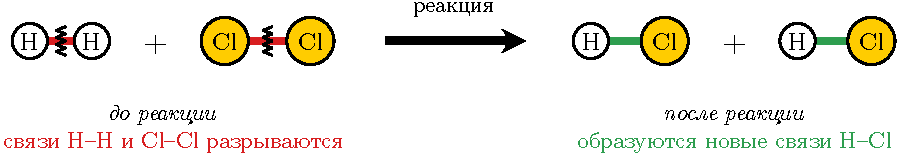
\includegraphics[width=\linewidth]{figs/enthalpy/bonds_break_and_form.pdf}
    \caption{Разрыв старых и образование новых связей при химической реакции.}
    \label{fig:bonds_break_and_form}
\end{figure}

Поскольку химические связи в исходных веществах и продуктах имеют разную энергию, то в процессе реакции будет выделяться или поглощаться энергия в зависимости от того, какова будет суммарная разница между энергиями разорванных и образованных связей\footnote{Строго говоря, это приближение, поскольку нужно учитывать более сложную картину. Связи имеют различные энергии в зависимости от того, в каком соединении они находятся, поэтому табличные энергии связей усреднены из данных по разным соединениям. При реакции также меняется энергия межмолекулярного взаимодействия и может происходить фазовый переход. Пока что, для понимания процесса, мы сосредоточимся на главном вкладе в изменение энергии.}.

Куда будет деваться выделяющаяся энергия (или откуда она будет браться) в случае разницы в суммарной энергии старых и новых связей? В этом случае будет происходить обмен энергией с окружением, либо энергия останется в системе (но тогда изменится температура). Поэтому важно понимать, что химические реакции не живут <<сами в себе>>, а являются частью общих процессов, и нужно всегда рассматривать их вместе с условиями, в которых они протекают.

Согласно первому началу термодинамики, внутренняя энергия закрытой системы может быть изменена путём теплопередачи или путём работы. Первая часть вклада~--- теплопередача~--- практически всегда присутствует при протекании реакций.

Тем не менее в лабораторных или промышленных условиях можно смоделировать так называемую \term{адиабатическую реакцию}{adiabatic_reaction}{адиабатическая реакция}, которая протекает в сосуде с хорошей теплоизоляцией при отсутствии теплообмена с окружением.

Вторая часть~--- работа~--- в зависимости от условий может либо иметь несущественную величину, либо иметь значительный вклад в том случае, если меняется объём реагирующей системы против внешнего давления (рис.~\ref{fig:energy_of_reaction}), или когда реакция сопряжена с работой иного рода.

\begin{figure}[htbp]
    \centering
    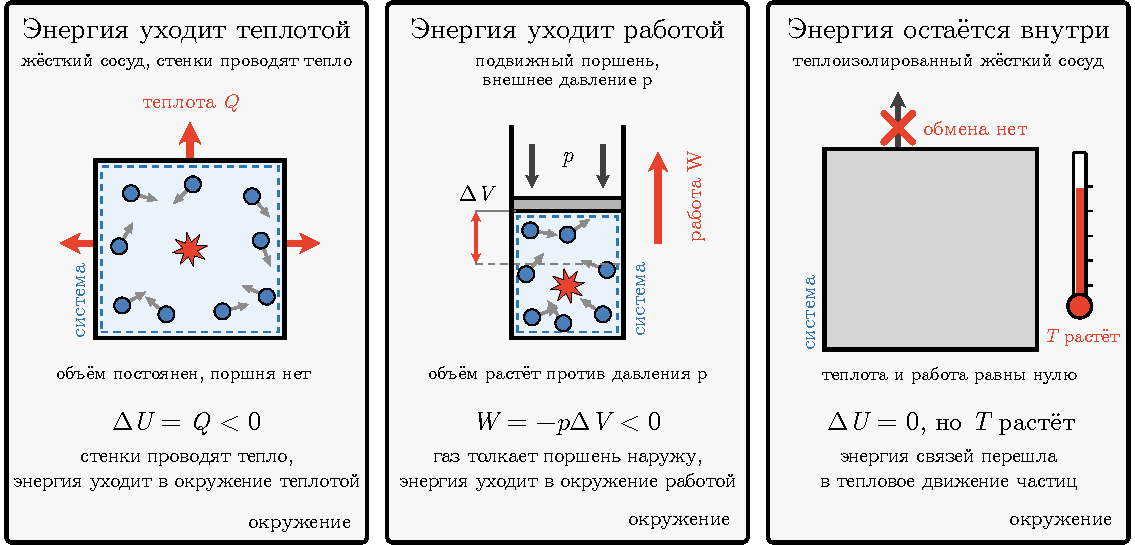
\includegraphics[width=\linewidth]{figs/enthalpy/energy_of_reaction.pdf}
    \caption{Экзотермическая реакция в закрытой системе: куда девается выделившаяся энергия. Левая панель: температура не изменяется, внутренняя энергия уменьшается из-за ушедшей теплоты. Центральная панель: температура не изменяется, внутренняя энергия уменьшается из-за совершённой работы. Правая панель: внутренняя энергия не изменяется, но перегруппировывается~--- запасённая химическая энергия перейдёт в кинетическую энергию молекул и температура повысится.}
    \label{fig:energy_of_reaction}
\end{figure}

Наиболее часто при химических реакциях встречается \term{работа расширения}{expansion_work}{работа расширения} (она имеет существенную величину, если образуются или расходуются газообразные вещества). Она равна произведению постоянного внешнего давления на изменение объёма, взятому со знаком минус,~--- при расширении система отдаёт энергию, поэтому $W < 0$:

\begin{equation*}
    W = -p\Delta{}V.
\end{equation*}

\subsection*{Почему нельзя просто использовать теплоту, чтобы описать изменение энергии при химической реакции?}

Теплота~--- это не свойство системы, а способ передачи энергии. Поэтому она является \term{функцией процесса}{process_function}{функция процесса}, или, простыми словами, зависит от пути реакции: того, при каких условиях она будет проведена.

К примеру, мы проводим одну и ту же реакцию в запаянном и в открытом сосудах. Исходные вещества и продукты вроде бы одни и те же, а вот количество теплоты при этом выделится разное. Это происходит потому, что реакция проведена при разных условиях: в первом случае вся выделившаяся энергия ушла в теплоту, после того как система вернулась к исходной температуре (рис.~\ref{fig:energy_of_reaction}, первая панель), а во втором часть энергии ушла на работу против внешнего давления~--- либо, наоборот, окружение само совершило работу над системой и добавило ей энергии (рис.~\ref{fig:energy_of_reaction}, вторая панель).

Поэтому нельзя создать справочную таблицу, в которой мы сможем записать <<теплота этой реакции такая-то>>~--- нужно обязательно указывать условия.

В отличие от теплоты как функции процесса, \term{функции состояния}{state_function}{функция состояния} зависят только от начального и конечного состояния системы, а не от пути, по которому система пришла из начальной точки в конечную. Например, внутренняя энергия $U$~--- это функция состояния.

Но тут возникает вопрос удобства этих функций.

Для химика, изучающего реакцию, неудобно каждый раз учитывать работу расширения, зато сравнительно легко измерить теплоту, выделяющуюся или поглощающуюся в ходе реакции.

Для того чтобы измеряемая теплота отражала изменение какой-либо функции состояния, мы должны зафиксировать некоторые условия проведения реакции. Например, если реакция проводится при постоянном объёме ($V = \mathrm{const}$), работа расширения будет равна нулю, и если система не совершает никакой другой работы (например, электрической), то вся измеренная теплота будет равна изменению внутренней энергии $\Delta{}U$.

Более распространённый на практике вариант~--- это реакция в открытой колбе при постоянном внешнем давлении ($p = \mathrm{const}$). В этом случае из измеренной теплоты тоже можно будет извлечь изменение функции состояния, но для этого нам потребуется ввести новую термодинамическую функцию. Именно она и называется энтальпией. Давайте разбираться, что это за функция.

\subsection*{Что такое энтальпия}

\term{Энтальп\'{и}я}{enthalpy}{энтальпия}~--- это термодинамическая функция, равная сумме внутренней энергии системы и произведения давления системы на её объём:

\begin{equation*}
    H = U + pV.
\end{equation*}

Изменение энтальпии в химической реакции равно:

\begin{equation*}
    \Delta{}H = \Delta{}U + \Delta{}(pV).
\end{equation*}

Поскольку нас интересуют реакции при постоянном давлении (а это, повторимся, подавляющее большинство химических реакций: в открытых сосудах, биохимические, в горных породах на поверхности Земли), формулу выше можно упростить до

\begin{equation*}
    \Delta{}H = \Delta{}U + p\Delta{}V.
\end{equation*}

Член $p\Delta{}V$~--- это уже упомянутая работа, которую система совершает над окружением при расширении из-за изменения числа молекул газа до и после реакции (рис.~\ref{fig:pressure_volume_work}). Это имеет смысл в первую очередь для процессов в газовой фазе, потому что в этих реакциях значительно меняется объём системы, если меняется общее число молей газа. Напомним, что объём идеальных газов при постоянном давлении и температуре пропорционален числу молекул газа, поэтому

\begin{equation*}
    \Delta{}V = \frac{\Delta{}n(\text{газ}) \cdot RT}{p}.
\end{equation*}

И, следовательно ($W$~--- работа, совершаемая \emph{над} системой):

\begin{equation*}
    W = -\Delta{}n(\text{газ}) \cdot RT.
\end{equation*}

\begin{figure}[htbp]
    \centering
    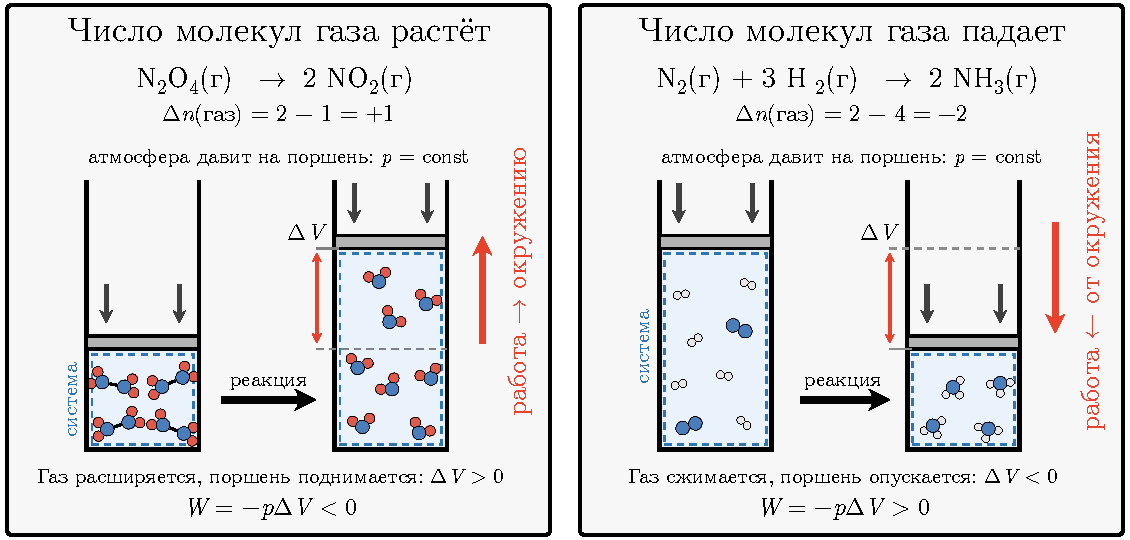
\includegraphics[width=\linewidth]{figs/enthalpy/pressure_volume_work.pdf}
    \caption{Если происходит расширение системы, то она совершает работу над окружением, а если сжатие, то наоборот.}
    \label{fig:pressure_volume_work}
\end{figure}

Для реакций твёрдых и жидких веществ объём системы тоже изменяется, но так незначительно\footnote{Вклад $p\Delta{}V$ для таких реакций на несколько порядков меньше, чем для реакций с участием газов.}, что этим изменением можно пренебречь в практических расчётах.

Первое начало термодинамики говорит нам, что $\Delta{}U = Q + W$. Если система не совершает никакой работы, кроме работы расширения ($W = -p\Delta{}V$), то $Q = \Delta{}U + p\Delta{}V$. Правая часть этого выражения~--- это и есть по определению изменение энтальпии при постоянном давлении. Другими словами, если реакция проводится при постоянном давлении, то изменение энтальпии равно теплоте, поглощённой в ходе реакции:

\begin{equation*}
   \Delta{}H = Q.
\end{equation*}

Это справедливо для любой реакции, идущей при постоянном давлении,~--- и в открытой колбе, и при изменении объёма газов (если только система не совершает работы иного рода, кроме расширения, см. ниже).

Энтальпия позволяет оценивать изменение энергии системы в химической реакции, идущей при постоянном давлении, на основании известных энергий связи (рис.~\ref{fig:enthalpy_bond_energy}). Кроме того, мы можем рассчитывать для таких реакций количество выделившейся или поглощённой теплоты, зная только исходные и конечные вещества.

\begin{figure}[htbp]
    \centering
    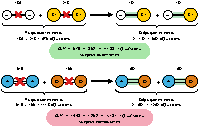
\includegraphics[width=\linewidth]{figs/enthalpy/enthalpy_bond_energy.pdf}
    \caption{Изменение энтальпии при химической реакции.}
    \label{fig:enthalpy_bond_energy}
\end{figure}

Впрочем, помните, что работа расширения~--- это не единственный возможный вид работы при химической реакции (см. табл.~\ref{tab:types_of_work}). Если система совершает ещё какую-то работу $A'$ (напомним, $A'$~--- работа, совершаемая системой, а $W$~--- над системой), то $Q = \Delta{}U + p\Delta{}V + A' = \Delta{}H + A'$, и тогда $Q \neq \Delta{}H$. Вот примеры таких процессов:

\begin{itemize}
    \item \textit{Гальванический элемент}. Если провести реакцию, положенную в его основу, без снятия электроэнергии, то всё изменение энтальпии проявится как выделившаяся теплота. В самом же элементе большая часть энергии уходит на электрическую работу, а разогрев системы очень слаб.
    \item \textit{Электролиз}. В этом случае, наоборот, окружение совершает работу над системой.
    \item \textit{Хемилюминесценция}. Часть энергии реакции уходит в виде излучения, а не тепла. Строго говоря, это не работа, а отдельный канал оттока энергии, но на баланс он влияет так же.
\end{itemize}

Если в реакцию не вступают газы и не образуется газообразных продуктов, то $\Delta{}(pV) \approx 0$, и тогда $\Delta{}H \approx \Delta{}U$; в этом случае теплота реакции при постоянном давлении практически совпадает с теплотой, которая выделилась бы или поглотилась при постоянном объёме.

Если энергия, необходимая для разрыва связей при химической реакции, больше энергии, выделяющейся при образовании связей, то изменение энтальпии реакции положительно ($\Delta{}H > 0$). При этом для протекания реакции требуется приток энергии: она поглощается системой из окружения, обеспечивая необходимое для реакции суммарное увеличение энергии. Такие реакции называют \term{эндотермическими}{endothermic_reaction}{эндотермическая реакция}.

Если энергия, необходимая для разрыва связей, меньше энергии, выделяющейся при образовании связей, то изменение энтальпии реакции отрицательно ($\Delta{}H < 0$). В этом случае при образовании продуктов возникает избыток энергии, который может быть передан системой окружению. Это \term{экзотермические}{exothermic_reaction}{экзотермическая реакция} реакции.

\begin{termlist}
    \hyperref[term:adiabatic_reaction]{Адиабатическая реакция},
    \hyperref[term:expansion_work]{работа расширения},
    \hyperref[term:process_function]{функция процесса},
    \hyperref[term:state_function]{функция состояния},
    \hyperref[term:enthalpy]{энтальпия},
    \hyperref[term:endothermic_reaction]{эндотермическая реакция},
    \hyperref[term:exothermic_reaction]{экзотермическая реакция}.
\end{termlist}

\begin{problem}{}{enthalpy1}
    Зависит ли работа расширения от давления, при котором идёт реакция?
    \begin{sol}{\ref{prob:enthalpy1}}
        До реакции объём газов составлял $V_1 = \frac{n_1RT}{p}$, после реакции $V_2 = \frac{n_2RT}{p}$. Тогда:
        \begin{equation*}
            \Delta{}V = \frac{(n_2 - n_1) \cdot RT}{p} = \frac{\Delta{}n(\text{газ}) \cdot RT}{p}.
        \end{equation*}
        Чтобы найти работу расширения, умножаем $\Delta{}V$ на $p$, и оказывается, что работа расширения не зависит от давления в системе:
        \begin{equation*}
            W = -p\Delta{}V = -\Delta{}n(\text{газ}) \cdot RT.
        \end{equation*}
        То есть при вдвое большем давлении объём меняется ровно вдвое слабее, а произведение $p\Delta{}V$ остаётся тем же.
    \end{sol}
\end{problem}

\begin{problem}{}{enthalpy2}
    Для каких из приведённых реакций теплота, измеренная при постоянном объёме, совпадёт с теплотой при постоянном давлении? Расположите остальные по возрастанию $\left|\Delta{}H - \Delta{}U\right|$, не вычисляя $\Delta{}H$.
    \begin{enumerate}[label=\arabic*)]
        \item \ce{H2_{(\text{г})} + Cl2_{(\text{г})} -> 2HCl_{(\text{г})}};
        \item \ce{C_{(\text{тв})} + O2_{(\text{г})} -> CO2_{(\text{г})}};
        \item \ce{2C_{(\text{тв})} + O2_{(\text{г})} -> 2CO_{(\text{г})}};
        \item \ce{N2_{(\text{г})} + 3H2_{(\text{г})} -> 2NH3_{(\text{г})}};
        \item \ce{CaCO3_{(\text{тв})} -> CaO_{(\text{тв})} + CO2_{(\text{г})}}.
    \end{enumerate}
    \begin{sol}{\ref{prob:enthalpy2}}
        Разность определяется только тем, меняется ли число молей газа в системе:
        \begin{equation*}
            \Delta{}H - \Delta{}U = \Delta{}n(\text{газ}) \cdot RT.
        \end{equation*}
        При комнатной температуре $RT \approx \qty{2,5}{\ruKJ\per\ruMole}$.

        Теплоты совпадают в случае реакций 1 и 2, для них $\Delta{}n(\text{газ}) = 0$. В реакциях 3 и 5 $\Delta{}n(\text{газ}) = +1$ (\qty{2,5}{\ruKJ\per\ruMole}), а в реакции 4 при $\Delta{}n(\text{газ}) = -2$~--- вдвое больше, \qty{5,0}{\ruKJ\per\ruMole}.
        Реакции по возрастанию модуля разности $\left|\Delta{}H - \Delta{}U\right|$: 3 и 5 (одинаково), затем 4.
    \end{sol}
\end{problem}

\clearpage

\section{Как использовать энтальпию}

Теперь после того, как мы изучили понятие энтальпии, возникает вопрос: как использовать её на практике?

Как мы уже выяснили, энтальпию как термодинамическую функцию ввели, чтобы для реакций, происходящих в изобарных условиях (самых распространённых в природе), перейти от теплоты как функции процесса к функции состояния, которой и является энтальпия. Это позволяет нам рассчитывать изменение энтальпии (считай~--- теплоты) для любой химической реакции на основании справочных данных, зная только об участвующих в реакции веществах.

В целом области применения энтальпии (подробнее некоторые из них мы разберём далее) следующие:

\begin{itemize}
    \item всё многообразие инженерных расчётов теплот процессов для последующего инженерного проектирования, например, расчёт теплот сгорания топлива, фазовых переходов в холодильной технике, процессов в химических реакторах и тепловых машинах и пр.;
    \item оценка стабильности химических соединений;
    \item определение пищевой ценности продуктов в пищевой промышленности.
\end{itemize}

Изменение энтальпии равно теплоте, поглощённой системой в ходе химической реакции в том случае, если давление в системе постоянно и равно внешнему, а система не совершает никакой другой работы, кроме работы расширения. Однако, чтобы стандартизировать величины энтальпии, мы должны зафиксировать не только постоянство давления, но и его конкретное значение, а также агрегатное состояние веществ и пр. Поэтому прежде всего давайте познакомимся с так называемыми \emph{стандартными состояниями}.

\subsection*{Что такое стандартные состояния}

Для корректного сравнения значений термодинамических функций состояния вводят \emph{опорные точки}~--- параметры состояния веществ, для которых договариваются указывать значения энергий. Эти состояния и называют \term{стандартными состояниями}{standard_state}{стандартное состояние}.

Принятые стандартные состояния приведены в таблице~\ref{tab:standard_states}.

\begin{table}[htbp]
    \small
    \caption{Стандартные состояния веществ.}
    \label{tab:standard_states}
    \begin{tabularx}{\textwidth}{
        >{\hsize=0.6\hsize}Y
        >{\hsize=1.4\hsize}Y
        }
        \hline
        \rowcolor{green!5}
        Вещество & Стандартное состояние \\
        \hline
        Твёрдое вещество & Чистое твёрдое вещество при давлении \qty{1}{\ruBar}, наиболее устойчивая форма (для простых веществ~--- аллотропная модификация) \\
        \hline
        Жидкость & Чистая жидкость при давлении \qty{1}{\ruBar} \\
        \hline
        Растворённое вещество & Концентрация \qty{1}{\ruMolar}, идеальный раствор \\
        \hline
        Газ & Чистый идеальный газ при давлении \qty{1}{\ruBar} \\
        \hline
    \end{tabularx}
\end{table}

\emph{Идеальные состояния} раствора и газа означают, что частицы в них не взаимодействуют друг с другом, а у газов частицы к тому же имеют пренебрежимо малый собственный объём.

Реальный газ всё больше ведёт себя как идеальный при уменьшении давления и становится идеальным при бесконечно малом давлении ($p \rightarrow 0$). Реальный раствор ведёт себя идеально при бесконечном разбавлении ($c \rightarrow 0$), при этом считается, что каждая частица растворённого вещества взаимодействует только с растворителем, но не с соседними растворёнными частицами. Задавать опорную точку при нулевом давлении или нулевой концентрации физически бессмысленно, поэтому берут идеальное поведение из области разбавления и представляют, что вещество ведёт себя так же и при давлении \qty{1}{\ruBar} (для газа) или концентрации \qty{1}{\ruMole\per\ruL} (для растворённого вещества).

Для чего нужны такие ухищрения? Поведение идеального газа и идеального раствора, в отличие от реальных, описывается гораздо более простыми формулами. При описанном выборе опорных точек эти простые формулы будут выполняться в стандартном состоянии точно, а все отклонения реального вещества от них можно математически вынести в отдельный поправочный множитель\footnote{\emph{Коэффициент летучести} для газов и \emph{коэффициент активности} для растворов.}.

Насколько это важно на практике? Для энтальпии эти приближения почти не оказывают влияния, потому что у идеального газа энтальпия вообще не зависит от давления\footnote{Почему, можете спросить вы, ведь по определению энтальпии $H = U + pV$? Дело в том, что в $H$ входит не давление само по себе, а произведение $pV$~--- и для идеального газа оно равно $nRT$, то есть зависит только от температуры. Второе слагаемое, $U$, для идеального газа тоже зависит только от температуры. Внутренняя энергия складывается из кинетической энергии молекул (она задаётся $T$) и потенциальной энергии их взаимодействия~--- а у идеального газа взаимодействий нет по определению. Раздвинуть молекулы, которые друг друга не притягивают, ничего не стоит.}, а отклонение реального газа от идеального при \qty{1}{\ruBar} пренебрежимо мало. А вот для растворов электролитов, где ионы заметно взаимодействуют уже при куда меньших концентрациях, чем \qty{1}{\ruMole\per\ruL}, разница между реальным и стандартным состоянием существенна.

Отдельно оговаривается так называемое \term{биохимическое стандартное состояние}{biochemical_standard_state}{биохим. станд. сост.}, при котором для растворённых веществ концентрация равна \qty{1}{\ruMolar}, за исключением \ce{[H+]}, которая равна \qty{1e-7}{\ruMolar}\footnote{Дело в том, что концентрация \ce{[H+] = \qty{1}{\ruMolar}} соответствует слишком кислому раствору ($\mathrm{pH} = 0$), который не встречается в реальных биологических процессах.}.

То, что измерения выполнены для стандартных состояний веществ, указывается символом $\circ$ в виде надстрочного индекса (например, $\Delta H^{\circ}$ или $\Delta H^{\circ\prime}$ для биохимического стандартного состояния).

Температура не оговорена в стандартных состояниях, но её также обычно указывают, поскольку она влияет на величины термодинамических функций из-за наличия у веществ теплоёмкости\footnote{Если вам интересно, изучите информацию о законе Кирхгофа в интернете.}. Обычно измерения проводят при комнатной температуре, равной \qty{25}{\degreeCelsius} (\qty{298,15}{\ruK}).

\subsection*{Закон Гесса}

То, что энтальпия и внутренняя энергия являются функциями состояния, а не процесса, лежит в основе \term{закона Гесса}{law_of_Hess}{закон Гесса}\footnote{Любопытно, что Герман Иванович Гесс установил свой закон эмпирически в 1840 году~--- за несколько лет до того, как было сформулировано первое начало термодинамики. Сегодня мы получаем закон Гесса как прямое следствие первого начала, но исторически всё было ровно наоборот.}: \emph{тепловой эффект химической реакции, проводимой в изобарно-изотермических или изохорно-изотермических условиях, зависит только от вида и состояния исходных веществ и продуктов реакции и не зависит от пути её протекания}. Как и раньше, подразумевается, что система не совершает никакой работы, кроме работы расширения.

Слово <<изотермических>> вовсе не означает, что температура обязана быть постоянной на всём пути: реакция может идти и с сильным разогревом. Самое главное, чтобы в конце продукты были приведены к той же температуре, что и исходные вещества.

Если переформулировать закон Гесса простыми словами, превращение одних веществ в другие посредством цепочки химических реакций сопровождается одним и тем же общим изменением энтальпии независимо от того, через какие промежуточные продукты мы это превращение провели (рис.~\ref{fig:hess_law_parallel_paths}).

\begin{figure}[htbp]
    \centering
    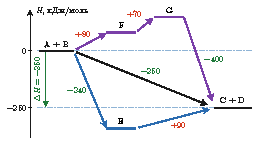
\includegraphics[width=10cm]{figs/how_to_use_enthalpy/hess_law_parallel_paths.pdf}
    \caption{Иллюстрация закона Гесса на примере реакции \ce{A + B -> C + D}. Реакция может идти разными путями, но суммарное изменение энтальпии окажется одинаковым.}
    \label{fig:hess_law_parallel_paths}
\end{figure}

Уравнения химических реакций, в которых дополнительно указаны агрегатные состояния всех участников и тепловой эффект, называют \term{термохимическими уравнениями}{thermochemical_equation}{термохимич. уравнение}. Например:

\reaction*{C_{(\text{графит})} + O2_{(\text{г})} -> CO2_{(\text{г})}, \quad $\Delta H^{\circ} = \qty{-393,5}{\ruKJ\per\ruMole}${.}}

В термохимических уравнениях допускаются дробные коэффициенты, к примеру, чтобы уравнение приводило к образованию \qty{1}{\ruMole} исследуемого вещества, а также для того, чтобы с такими уравнениями было удобно работать алгебраически (складывать друг с другом или вычитать).

\begin{example}{}{how_to_use_enthalpy1}
    \begin{condition}
        Найдите тепловой эффект реакции образования \ce{CO}:
        \reaction*{C_{(\textup{графит})} + \frac{1}{2}O2_{(\textup{г})} -> CO_{(\textup{г})}{.}}
    \end{condition}

    \medskip

    \textit{Решение.} Измерить тепловой эффект такой реакции напрямую невозможно, потому что углерод на практике всегда сгорает с образованием смеси \ce{CO} и \ce{CO2}, и измерения покажут теплоту образования этой смеси, точный состав которой неизвестен.

    Однако мы можем легко провести две другие реакции, которые идут без образования побочных продуктов, и измерить их тепловой эффект:

    \reaction*{\text{(1)} \quad C_{(\text{графит})} + O2_{(\text{г})} -> CO2_{(\text{г})}, \quad \Delta H_1 = \qty{-393,5}{\ruKJ\per\ruMole}{,}}
    \reaction*{\text{(2)} \quad CO_{(\text{г})} + \frac{1}{2}O2_{(\text{г})} -> CO2_{(\text{г})}, \quad \Delta H_2 = \qty{-283,0}{\ruKJ\per\ruMole}{.}}

    Таким образом, перейти от углерода и кислорода к \ce{CO2} можно двумя путями~--- напрямую или через две последовательные реакции с образованием \ce{CO}. Начальное и конечное состояния у обоих путей одинаковые, значит, согласно закону Гесса одинаковы и суммарные изменения энтальпии по обоим путям:

    \begin{equation*}
        \Delta H_1 = \Delta H_{\text{иск.}} + \Delta H_2.
    \end{equation*}

    Отсюда

    \begin{equation*}
        \Delta H_{\text{иск.}} = \Delta H_1 - \Delta H_2 = \num{-393,5} - (\num{-283,0}) = \qty{-110,5}{\ruKJ\per\ruMole}.
    \end{equation*}
\end{example}

\subsection*{Энтальпии образования и сгорания}

Итак, теперь мы можем использовать закон Гесса для того, чтобы вычислять неизвестный тепловой эффект исходя из изменений энтальпий известных реакций. Однако как теперь провести стандартизацию, чтобы для любой не особенно экзотической химической реакции у нас были опорные данные по энтальпии для участвующих в ней веществ?

Поскольку абсолютные значения энтальпии неизвестны и мы вынуждены оперировать \emph{изменениями} энтальпии, в качестве такой опорной точки для отдельных веществ были взяты так называемые \emph{реакции образования} и \emph{сгорания} веществ. Они представляют собой унифицированные реакции, изменения энтальпии которых приводятся в справочниках, и которые можно использовать для расчёта изменения энтальпии других реакций.

\term{Реакция образования вещества}{formation_reaction}{реакция образования}~--- это реакция, в которой один моль данного вещества образуется из простых веществ, взятых в их наиболее устойчивых при данных условиях формах.

Примеры реакций образования:

\ce{C_{(\text{графит})} + \frac{1}{2}O2_{(\text{г})} -> CO_{(\text{г})}{,} \quad $\Delta{}_fH^{\circ} = \qty{-110,5}{\ruKJ\per\ruMole}$};

\ce{H2_{(\text{г})} + \frac{1}{2}O2_{(\text{г})} -> H2O_{(\text{ж})}{,} \quad $\Delta{}_fH^{\circ} = \qty{-285,8}{\ruKJ\per\ruMole}$};

\ce{\frac{1}{2}N2_{(\text{г})} + \frac{3}{2}H2_{(\text{г})} -> NH3_{(\text{г})}{,} \quad $\Delta{}_fH^{\circ} = \qty{-45,9}{\ruKJ\per\ruMole}$}.

Изменения энтальпии в этих реакциях называют \term{энтальпиями образования}{enthalpy_of_formation}{энтальпия образования} и обозначают буквой \textit{f} (от англ. <<\textit{formation}>>), например, $\Delta{}_fH_{\num{298,15}}^{\circ}(\ce{H2O}, \text{ж}) = \qty{-285,8}{\ruKJ\per\ruMole}$.

Энтальпия образования простых веществ в их наиболее устойчивой форме по определению равна нулю.

\term{Реакция сгорания вещества}{combustion_reaction}{реакция сгорания}~--- это реакция полного окисления одного моля вещества избытком кислорода, в которой каждый входящий в вещество элемент переходит в строго определённый продукт сгорания.

Примеры реакций сгорания:

\ce{CH4_{(\text{г})} + 2O2_{(\text{г})} -> CO2_{(\text{г})} + 2H2O_{(\text{ж})}{,} \quad $\Delta{}_cH^{\circ} = \qty{-890,5}{\ruKJ\per\ruMole}$};

\ce{C2H5OH_{(\text{ж})} + 3O2_{(\text{г})} -> 2CO2_{(\text{г})} + 3H2O_{(\text{ж})}{,} \quad $\Delta{}_cH^{\circ} = \qty{-1366,8}{\ruKJ\per\ruMole}$};

\ce{C6H12O6_{(\text{тв})} + 6O2_{(\text{г})} -> 6CO2_{(\text{г})} + 6H2O_{(\text{ж})}{,} \quad $\Delta{}_cH^{\circ} = \qty{-2802,5}{\ruKJ\per\ruMole}$}.

Изменения энтальпии в этих реакциях называют \term{энтальпиями сгорания}{enthalpy_of_combustion}{энтальпия сгорания} и обозначают буквой \textit{c} (от англ. <<\textit{combustion}>>), например, $\Delta{}_cH_{\num{298,15}}^{\circ}(\ce{CH4}, \text{г}) = \qty{-890,5}{\ruKJ\per\ruMole}$.

Теплота сгорания уже сгоревшего вещества (\ce{H2O}, \ce{CO2}) равна нулю.

Теперь, зная теплоты образования или сгорания всех веществ, участвующих в любой химической реакции, мы можем рассчитать её тепловой эффект с использованием \emph{четырёх следствий из закона Гесса}:

\emph{Следствие 1. Тепловой эффект обратной реакции равен по величине и противоположен по знаку тепловому эффекту прямой реакции:}

\begin{equation*}
    \Delta H(\text{обратной}) = -\Delta H(\text{прямой}).
\end{equation*}

Это утверждение известно как \emph{закон Лавуазье~--- Лапласа}\footnote{Сформулирован в 1780 году, за шестьдесят лет до закона Гесса. Сегодня его удобнее выводить как следствие, но исторически он был установлен независимо и раньше.}.

Практический смысл этого следствия в том, что термохимическое уравнение можно разворачивать, меняя знак теплового эффекта. Это позволяет обращаться с термохимическими уравнениями как с алгебраическими: складывать их, вычитать, умножать на числа.

\emph{Следствие 2. Если начальное и конечное состояния совпадают, суммарный тепловой эффект равен нулю.}

Иначе говоря, тепловой эффект любого циклического процесса равен нулю. На первый взгляд, это утверждение выглядит довольно очевидным, однако оно лежит в основе техники термохимических циклов, когда, замкнув цепочку реакций в кольцо и приравняв сумму к нулю, мы получаем уравнение, из которого находится любое одно неизвестное звено. Рассмотрим такой подход на примере ниже.

\begin{example}{}{how_to_use_enthalpy2}
    \begin{condition}
        Рассчитайте энергию кристаллической решётки \ce{NaCl}.
    \end{condition}

    \medskip

    \textit{Решение.} Энергия кристаллической решётки~--- это тепловой эффект превращения
    \reaction*{Na^+_{(\text{г})} + Cl^-_{(\text{г})} -> NaCl_{(\text{кр})}{,}}
    то есть энергия, выделяющаяся при сборке кристалла из бесконечно удалённых друг от друга газообразных ионов. Измерить её напрямую невозможно~--- нельзя взять кристалл поваренной соли и в эксперименте развести его ионы на бесконечность, получив газ из \ce{Na^+} и \ce{Cl^-}.

    Однако заметим, что от натрия и хлора к кристаллу \ce{NaCl} ведут два пути.

    Путь 1, прямой~--- сгорание натрия в хлоре:
    \reaction*{Na_{(\text{кр})} + \frac{1}{2}Cl2_{(\text{г})} -> NaCl_{(\text{кр})}{,} \quad $\Delta{}_fH^{\circ} = \qty{-411,2}{\ruKJ\per\ruMole}${.}}
    Путь 2, через газообразные ионы (цикл Борна~--- Габера): сначала превратить оба простых вещества в свободные атомы, затем в ионы, а уже потом собрать из них кристалл:
    \begin{center}
        \small
        \begin{tabularx}{\linewidth}{
            >{\hsize=1.2\hsize}Y
            >{\hsize=0.8\hsize}Y
            }
            \hline
            \rowcolor{green!5}
            Стадия & $\Delta H^\circ$, \unit{\ruKJ\per\ruMole} \\
            \hline
            \ce{Na_{(\text{кр})} -> Na_{(\text{г})}}~--- сублимация натрия & $+\num{107,5}$ \\
            \hline
            \ce{Na_{(\text{г})} -> Na^+_{(\text{г})} + e^-}~--- ионизация & $+\num{495,8}$ \\
            \hline
            \ce{\frac{1}{2}Cl2_{(\text{г})} -> Cl_{(\text{г})}}~--- разрыв половины связи \ce{Cl\bond{1}Cl} & $+\num{121,3}$ \\
            \hline
            \ce{Cl_{(\text{г})} + e^- -> Cl^-_{(\text{г})}}~--- присоединение электрона & $-\num{349,0}$ \\
            \hline
            \ce{Na^+_{(\text{г})} + Cl^-_{(\text{г})} -> NaCl_{(\text{кр})}}~--- сборка решётки & $\Delta{}_\text{реш}H^{\circ} = \text{?}$ \\
            \hline
        \end{tabularx}
    \end{center}
    Начальное и конечное состояния у обоих путей одинаковые, значит, по закону Гесса одинаковы и изменения энтальпии:
    \begin{equation*}
        \Delta{}_fH^{\circ} = \num{107,5} + \num{495,8} + \num{121,3} - \num{349,0} + \Delta{}_\text{реш}H^{\circ};
    \end{equation*}
    \begin{equation*}
        -\num{411,2} = \num{375,6} + \Delta{}_\text{реш}H^{\circ};
    \end{equation*}
    \begin{equation*}
        \Delta{}_\text{реш}H^{\circ} = -\num{411,2} - \num{375,6} = \qty{-786,8}{\ruKJ\per\ruMole}.
    \end{equation*}
    Для первых четырёх стадий имеются экспериментальные данные, а пятая находится из цикла как единственное неизвестное. Обратите внимание, что в некоторой литературе энергией решётки считается положительной: \qty{786,8}{\ruKJ\per\ruMole}.
\end{example}

\emph{Следствие 3. Тепловой эффект реакции равен сумме энтальпий образования продуктов минус сумма энтальпий образования исходных веществ (с учётом стехиометрических коэффициентов).}

\begin{equation*}
    \Delta{}H^{\circ} = \sum n_{\text{прод}} \cdot \Delta{}_fH^{\circ}(\text{продукты}) - \sum n_{\text{исх}} \cdot \Delta{}_fH^{\circ}(\text{исходные вещества}).
\end{equation*}

Путь от реагентов к продуктам строится так (рис.~\ref{fig:hess_corollaries_3_4}):

\begin{itemize}
    \item Реагенты разлагаются на простые вещества. Это процесс, обратный образованию реагентов, поэтому берётся сумма энтальпий их образования со знаком минус: $-\sum \Delta{}_fH(\text{реаг.})$.
    \item Из простых веществ синтезируются продукты. Суммарный тепловой эффект равен $+\sum \Delta{}_fH(\text{прод.})$.
    \item Итоговая формула: $\Delta H = \sum \Delta{}_fH(\text{прод.}) - \sum \Delta{}_fH(\text{реаг.})$.
\end{itemize}

\emph{Следствие 4. Тепловой эффект реакции равен сумме теплот сгорания исходных веществ минус сумма теплот сгорания продуктов.}

\begin{equation*}
    \Delta{}H^{\circ} = \sum n_{\text{исх}} \cdot \Delta{}_cH^{\circ}(\text{исходные вещества}) - \sum n_{\text{прод}} \cdot \Delta{}_cH^{\circ}(\text{продукты}).
\end{equation*}

Путь от реагентов к продуктам строится так (рис.~\ref{fig:hess_corollaries_3_4}):

\begin{itemize}
    \item Реагенты полностью сжигаются до продуктов полного сгорания. Тепловой эффект будет равен $+\sum \Delta{}_cH(\text{реаг.})$.
    \item Из полученных продуктов сгорания <<собираются>> целевые продукты реакции. Это процесс, обратный сгоранию продуктов, поэтому берётся сумма их энтальпий сгорания со знаком минус: $-\sum \Delta{}_cH(\text{прод.})$.
    \item Итоговая формула: $\Delta H = \sum \Delta{}_cH(\text{реаг.}) - \sum \Delta{}_cH(\text{прод.})$.
\end{itemize}

\begin{figure}[htbp]
    \centering
    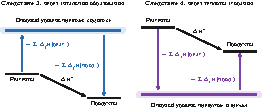
\includegraphics[width=\linewidth]{figs/how_to_use_enthalpy/hess_corollaries_3_4.pdf}
    \caption{Использование простых веществ и продуктов сгорания в качестве опорных точек при расчёте теплоты реакции.}
    \label{fig:hess_corollaries_3_4}
\end{figure}

Практическая ценность двух последних следствий для расчётов одинакова, но область применения разная. Для неорганических веществ обычно доступнее данные по энтальпии образования, а для органических~--- теплоты сгорания.

\begin{example}{}{how_to_use_enthalpy3}
    \begin{condition}
        Рассчитайте стандартный тепловой эффект разложения карбоната кальция:

        \reaction*{CaCO3_{(\textup{тв})} -> CaO_{(\textup{тв})} + CO2_{(\textup{г})}{,}}

        воспользовавшись справочными данными об энтальпиях образования:

        $\Delta{}_fH^{\circ}(\ce{CaCO3_{(\textup{тв})}}) = \qty{-1206,9}{\ruKJ\per\ruMole}$,

        $\Delta{}_fH^{\circ}(\ce{CaO_{(\textup{тв})}}) = \qty{-635,1}{\ruKJ\per\ruMole}$,

        $\Delta{}_fH^{\circ}(\ce{CO2_{(\textup{г})}}) = \qty{-393,5}{\ruKJ\per\ruMole}$.
    \end{condition}

    \medskip

    \textit{Решение.} Согласно третьему следствию закона Гесса:
    \begin{equation*}
        \Delta H^{\circ} = [\Delta{}_f H^{\circ}(\ce{CaO}) + \Delta{}_f H^{\circ}(\ce{CO2})] - \Delta{}_f H^{\circ}(\ce{CaCO3}).
    \end{equation*}
    \begin{equation*}
        \Delta H^{\circ} = [(\num{-635,1}) + (\num{-393,5})] - (\num{-1206,9}) = +\qty{178,3}{\ruKJ\per\ruMole}.
    \end{equation*}
    Положительный знак показывает, что разложение карбоната кальция эндотермично.
\end{example}

\begin{example}{}{how_to_use_enthalpy4}
    \begin{condition}
        Рассчитайте стандартный тепловой эффект превращения глюкозы в этанол и углекислый газ:

        \reaction*{C6H12O6_{(\textup{тв})} -> 2C2H5OH_{(\textup{ж})} + 2CO2_{(\textup{г})}{,}}

        воспользовавшись справочными данными по теплотам сгорания веществ:

        $\Delta{}_cH^{\circ}(\ce{C6H12O6_{(\textup{тв})}}) = \qty{-2802,5}{\ruKJ\per\ruMole}$,

        $\Delta{}_cH^{\circ}(\ce{C2H5OH_{(\textup{ж})}}) = \qty{-1366,8}{\ruKJ\per\ruMole}$.
    \end{condition}

    \medskip

    \textit{Решение.} Теплота сгорания углекислого газа по определению равна нулю. Составим выражение для расчёта теплового эффекта, воспользовавшись четвёртым следствием из закона Гесса:
    \begin{equation*}
        \Delta H^{\circ} = \Delta{}_cH^{\circ}(\ce{C6H12O6}) - [2\Delta{}_cH^{\circ}(\ce{C2H5OH}) + 2\Delta{}_cH^{\circ}(\ce{CO2})].
    \end{equation*}
    \begin{equation*}
        \Delta H^{\circ} = (\num{-2802,5}) - [2(\num{-1366,8}) + 2 \cdot 0] = \qty{-68,9}{\ruKJ\per\ruMole}.
    \end{equation*}
    Отрицательный знак показывает, что процесс экзотермичен.
\end{example}

\subsection*{Устойчивость соединений и самопроизвольность процессов}

Если в результате химической реакции энтальпия системы уменьшается ($\Delta H < 0$, экзотермическая реакция), то это означает, что система отдаёт энергию окружению. В эндотермической реакции наоборот~--- система поглощает энергию из окружения, в результате чего её энтальпия увеличивается.

Казалось бы, экзотермическая реакция приводит к продуктам, которые в целом устойчивее исходных соединений, а эндотермическая~--- наоборот, что позволяет нам сравнивать между собой различные формы одного и того же вещества. Но на самом деле это не так. Можно привести довольно много контрпримеров, например, переход ромбической серы в моноклинную эндотермичен ($\Delta H \approx +\qty{0,3}{\ruKJ\per\ruMole}$), однако выше \qty{95,3}{\degreeCelsius} устойчива именно моноклинная форма.

Дело в том, что нужно различать \emph{энергетическую} (прочность связей, запас потенциальной энергии) и \emph{термодинамическую устойчивость}. Энтальпия~--- важный, но не единственный вклад в устойчивость, поскольку необходимо учитывать также \emph{энтропию} соединений.

Энтальпия также не определяет \emph{самопроизвольность процессов}. По тому, выделяется теплота в процессе или поглощается, нельзя определить, будет ли происходить данный процесс самопроизвольно или нет, поскольку система будет двигаться в сторону именно термодинамической, а не энергетической устойчивости, например:

\begin{itemize}
    \item растворение \ce{NH4NO3} в воде сопровождается сильным поглощением теплоты, но при этом идёт самопроизвольно;
    \item таяние льда при $+\qty{5}{\degreeCelsius}$ происходит с поглощением теплоты, тем не менее оно тоже протекает само собой.
\end{itemize}

К устойчивости соединений и самопроизвольности процессов мы вернёмся дальше в этой же главе.

\subsection*{Как измерить изменение энтальпии}

Измерить энтальпию напрямую нельзя (кстати, сформулируйте самостоятельно, почему)~--- можно измерить лишь изменение энтальпии при протекании химической реакции.

Это можно сделать, например, проведя реакцию сжигания исследуемого вещества в специальном приборе~--- \term{калориметрической бомбе}{bomb_calorimeter}{калориметрическая бомба}, которая позволяет измерить теплоту, выделившуюся или поглотившуюся в ходе процесса. Устройство калориметрической бомбы представлено на рис.~\ref{fig:bomb_calorimeter}.

\begin{figure}[htbp]
    \centering
    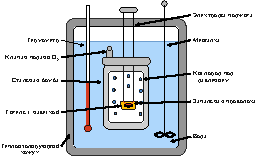
\includegraphics[width=\linewidth]{figs/how_to_use_enthalpy/bomb_calorimeter.pdf}
    \caption{Устройство калориметрической бомбы.}
    \label{fig:bomb_calorimeter}
\end{figure}

Навеску вещества помещают в тигель внутри бомбы~--- толстостенного стального сосуда,~--- после чего бомбу заполняют чистым кислородом (в избытке) под давлением около \qty{30}{\ruAtm}.

Бомбу погружают в воду известной массы, налитую в калориметрический сосуд, помещённый в теплоизолирующий кожух. Навеску поджигают, пропуская электрический ток через запальную проволоку с высоким удельным сопротивлением (например, нихромовую), натянутую между электродами над тиглем с навеской вещества.

Выделившаяся при сгорании теплота нагревает бомбу и воду. Прирост температуры фиксируется термометром; обычно он составляет несколько градусов, а измеряют его с точностью до тысячных долей градуса. Зная теплоёмкость всего калориметра (воды и бомбы), по приросту температуры вычисляют выделившуюся теплоту. Саму теплоёмкость определяют заранее, сжигая в том же приборе навеску эталонного вещества с известной теплотой сгорания (чаще всего бензойную кислоту).

Как вы можете заметить, реакция проводится при постоянном объёме, а не при постоянном давлении. Поэтому прямое измерение даёт нам величину изменения внутренней энергии ($\Delta U$), а не энтальпии. Для того чтобы пересчитать полученное значение в энтальпию, мы должны сделать поправку на гипотетическую работу расширения, которая была бы выполнена, если бы реакция проводилась при постоянном давлении:

\begin{equation*}
    \Delta H = \Delta U + \Delta n(\text{газ}) \cdot RT,
\end{equation*}

где $\Delta n(\text{газ})$~--- изменение числа молей газообразных веществ в реакции, которое находят по её уравнению.

\begin{termlist}
    \hyperref[term:standard_state]{Стандартное состояние},
    \hyperref[term:biochemical_standard_state]{биохимическое стандартное состояние},
    \hyperref[term:law_of_Hess]{закон Гесса},
    \hyperref[term:thermochemical_equation]{термохимическое уравнение},
    \hyperref[term:formation_reaction]{реакция образования},
    \hyperref[term:enthalpy_of_formation]{энтальпия образования},
    \hyperref[term:combustion_reaction]{реакция сгорания},
    \hyperref[term:enthalpy_of_combustion]{энтальпия сгорания},
    \hyperref[term:bomb_calorimeter]{калориметрическая бомба}.
\end{termlist}

\begin{problem}{}{how_to_use_enthalpy1}
    Среди представленных уравнений реакций выберите реакции образования:
    \begin{enumerate}[label=\arabic*)]
        \item \ce{\frac{1}{2}N2_{(\text{г})} + O2_{(\text{г})} -> NO2_{(\text{г})}};
        \item \ce{2Na_{(\text{кр})} + Cl2_{(\text{г})} -> 2NaCl_{(\text{кр})}};
        \item \ce{Ca_{(\text{кр})} + C_{(\text{графит})} + \frac{3}{2}O2_{(\text{г})} -> CaCO3_{(\text{тв})}};
        \item \ce{C_{(\text{алмаз})} + O2_{(\text{г})} -> CO2_{(\text{г})}};
        \item \ce{CO_{(\text{г})} + \frac{1}{2}O2_{(\text{г})} -> CO2_{(\text{г})}};
        \item \ce{H2_{(\text{г})} + \frac{1}{2}O2_{(\text{г})} -> H2O_{(\text{г})}};
        \item \ce{H2_{(\text{г})} + Br2_{(\text{г})} -> 2HBr_{(\text{г})}}.
    \end{enumerate}
    \begin{sol}{\ref{prob:how_to_use_enthalpy1}}
        Всем требованиям отвечают только уравнения 1, 3 и 6. В уравнении 2 образуются два моля \ce{NaCl} вместо одного. В уравнении 4 углерод взят в виде алмаза, хотя наиболее устойчивой формой при комнатной температуре является графит. В уравнении 5 слева стоит \ce{CO}~--- сложное вещество. В уравнении 7 образуются два моля продукта, кроме того, взят газообразный бром (при комнатной температуре бром~--- жидкость).
    \end{sol}
\end{problem}

\begin{problem}{}{how_to_use_enthalpy2}
    Среди представленных уравнений реакций выберите реакции сгорания:
    \begin{enumerate}[label=\arabic*)]
        \item \ce{2C2H2_{(\text{г})} + 5O2_{(\text{г})} -> 4CO2_{(\text{г})} + 2H2O_{(\text{ж})}};
        \item \ce{CH3OH_{(\text{ж})} + \frac{3}{2}O2_{(\text{г})} -> CO2_{(\text{г})} + 2H2O_{(\text{ж})}};
        \item \ce{H2_{(\text{г})} + \frac{1}{2}O2_{(\text{г})} -> H2O_{(\text{г})}};
        \item \ce{S_{(\text{ромбическая})} + \frac{3}{2}O2_{(\text{г})} -> SO3_{(\text{г})}};
        \item \ce{C2H5SH_{(\text{ж})} + \frac{9}{2}O2_{(\text{г})} -> 2CO2_{(\text{г})} + 3H2O_{(\text{ж})} + SO2_{(\text{г})}};
        \item \ce{CH4_{(\text{г})} + \frac{3}{2}O2_{(\text{г})} -> CO_{(\text{г})} + 2H2O_{(\text{ж})}};
        \item \ce{(NH2)2CO_{(\text{тв})} + \frac{3}{2}O2_{(\text{г})} -> CO2_{(\text{г})} + 2H2O_{(\text{ж})} + N2_{(\text{г})}}.
    \end{enumerate}
    \begin{sol}{\ref{prob:how_to_use_enthalpy2}}
        Реакциями сгорания, отвечающими всем требованиям, являются уравнения 2, 5 и 7. В уравнении 1 сгорает два моля ацетилена. В уравнении 3 вода газообразная, а не жидкая. В уравнении 4 продуктом реакции должен быть \ce{SO2}. В уравнении 6 окисление неполное.
    \end{sol}
\end{problem}

\begin{problem}{}{how_to_use_enthalpy3}
    Теплоты образования и сгорания~--- удобные, но не единственные возможные варианты опорных точек для термохимических расчётов. Предложите какие-нибудь другие варианты.
    \begin{sol}{\ref{prob:how_to_use_enthalpy3}}
        Выбор <<нулевого уровня>> зависит от того, какие частицы и процессы удобнее рассматривать в конкретной системе; главное, чтобы у всех веществ было общее состояние, к которому их можно привести. Можно использовать, например, полностью изолированные газообразные атомы, средние энергии связей, нейтральные частицы и свободный электрон в вакууме. Можно использовать не сгорание, а фторирование; в этом случае продуктами должны быть устойчивые фториды.
    \end{sol}
\end{problem}

\begin{problem}{}{how_to_use_enthalpy4}
    Рассчитайте тепловой эффект реакции:
    \reaction*{4NH3_{(\text{г})} + 5O2_{(\text{г})} -> 4NO_{(\text{г})} + 6H2O_{(\text{г})}{,}}
    используя стандартные теплоты образования: $\Delta{}_fH^{\circ}(\ce{NH3}, \text{г}) = \qty{-45,9}{\ruKJ\per\ruMole}$; $\Delta{}_fH^{\circ}(\ce{NO}, \text{г}) = +\qty{90,3}{\ruKJ\per\ruMole}$; $\Delta{}_fH^{\circ}(\ce{H2O}, \text{г}) = \qty{-241,8}{\ruKJ\per\ruMole}$.
    \begin{sol}{\ref{prob:how_to_use_enthalpy4}}
        Согласно третьему следствию из закона Гесса:
        \begin{align*}
            \Delta H^{\circ} &= [4 \cdot (+\num{90,3}) + 6 \cdot (\num{-241,8})] - [4 \cdot (\num{-45,9}) + 5 \cdot 0] = \\
            &= (\num{361,2} - \num{1450,8}) + \num{183,6} = \qty{-906,0}{\ruKJ\per\ruMole}.
        \end{align*}
    \end{sol}
\end{problem}

\begin{problem}{}{how_to_use_enthalpy5}
    После сжигания метана в калориметрической бомбе выделилось \qty{885,5}{\ruKJ\per\ruMole} теплоты:
    \reaction*{CH4_{(\text{г})} + 2O2_{(\text{г})} -> CO2_{(\text{г})} + 2H2O_{(\text{ж})}{.}}
    Найдите энтальпию сгорания метана.
    \begin{sol}{\ref{prob:how_to_use_enthalpy5}}
        Поскольку процесс был проведён в калориметрической бомбе, то измеренная теплота соответствует изменению внутренней энергии ($\Delta U = \qty{-885,5}{\ruKJ\per\ruMole}$). Чтобы перейти к энтальпии, необходимо сделать поправку на работу расширения за счёт изменения количества газообразных веществ. Согласно уравнению реакции $\Delta n(\text{газ}) = 1 - 3 = -2$, поэтому
        \begin{equation*}
            \Delta H = \Delta U + \Delta n(\text{газ}) \cdot RT = \num{-885,5} + (\num{-2}) \cdot \num{2,479} = \qty{-890,5}{\ruKJ\per\ruMole},
        \end{equation*}
        где $RT = \num{8,314} \cdot \num{298,15} = \qty{2479}{\ruJ\per\ruMole} \approx \qty{2,479}{\ruKJ\per\ruMole}$.

        Физический смысл разницы в значениях заключается в том, что система сжимается и окружение совершает над ней работу, поэтому теплоты при постоянном давлении выделяется больше, чем при постоянном объёме.
    \end{sol}
\end{problem}

\begin{problem}{}{how_to_use_enthalpy6}
    Пользуясь справочными данными по стандартным энтальпиям образования веществ, определите теплоту испарения воды.
    \begin{sol}{\ref{prob:how_to_use_enthalpy6}}
        Процесс соответствует схеме:
        \reaction*{H2O_{(\text{ж})} -> H2O_{(\text{г})}{.}}
        Не имеет значения, является процесс химической реакцией или фазовым превращением, для функций состояния важны только конечное и начальное состояния. Поэтому находим в справочниках стандартные энтальпии образования газообразной и жидкой воды и рассчитываем:
        \begin{equation*}
            \Delta H^{\circ} = \Delta{}_fH^{\circ}(\ce{H2O}, \text{г}) - \Delta{}_fH^{\circ}(\ce{H2O}, \text{ж}) = \num{-241,8} - (\num{-285,8}) = +\qty{44,0}{\ruKJ\per\ruMole}.
        \end{equation*}
        В справочной литературе для теплоты испарения воды обычно приводят не такое значение, а \qty{40,7}{\ruKJ\per\ruMole}. Эта величина относится к \emph{температуре кипения} воды. Теплота испарения зависит от температуры и убывает с её ростом, становясь равной нулю в так называемой \emph{критической точке}.
    \end{sol}
\end{problem}

\begin{problem}{}{how_to_use_enthalpy7}
    $\bigstar$ Профессор Недоумелкин недоумевает: его расчёты не совпадают с результатами эксперимента из задачи \ref{prob:how_to_use_enthalpy5}. Он заявляет вам, что у него получается \qty{-802,5}{\ruKJ\per\ruMole}, а не \qty{-890,5}{\ruKJ\per\ruMole}. Он дважды проверил расчёты и арифметических ошибок у него нет. В чём состояла его ошибка?
    \begin{sol}{\ref{prob:how_to_use_enthalpy7}}
        Расхождение значений составляет $\num{890,5} - \num{802,5} = \qty{88,0}{\ruKJ\per\ruMole}$. Можно догадаться, что это удвоенная теплота испарения воды (\qty{44,0}{\ruKJ\per\ruMole}). В уравнении реакции как раз фигурируют два моля воды. Получается, что Недоумелкин в расчёте использовал энтальпию образования водяного пара, а не жидкой воды:
        \begin{equation*}
            \Delta H^{\circ} = [\num{-393,5} + 2 \cdot (\num{-241,8})] - (\num{-74,6}) = \qty{-802,5}{\ruKJ\per\ruMole}.
        \end{equation*}
        Правильный расчёт совпадает с экспериментальными данными:
        \begin{equation*}
            \Delta H^{\circ} = [\num{-393,5} + 2 \cdot (\num{-285,8})] - (\num{-74,6}) = \qty{-890,5}{\ruKJ\per\ruMole}.
        \end{equation*}
    \end{sol}
\end{problem}

\clearpage

\section{Знакомство с энтропией}

Давайте представим себе две ситуации.

\emph{Ситуация первая.} Горячий предмет поставили в холодную комнату. Через некоторое время температуры предмета и комнаты сравнялись~--- энергия перешла от предмета (система) к комнате (окружение). Суммарная энергия предмета и комнаты при этом не изменилась.

Первое начало термодинамики (читай: закон сохранения энергии) не запрещает нам ни передачи энергии от горячего предмета к холодному, ни наоборот. Если бы комната сама собой немного охладилась, передав тепло предмету, который бы нагрелся за счёт этой теплоты ещё сильнее, ничего не было бы нарушено. Тем не менее даже из своего бытового опыта вы знаете, что ничего подобного не происходит никогда. Поэтому возникают два вопроса:

\begin{itemize}
    \item чем принципиально различаются начальное и конечное состояния, если энергия у них одна и та же?
    \item что задаёт направление передачи энергии?
\end{itemize}

\emph{Ситуация вторая.} Два одинаковых сосуда с теплоизолированными стенками соединены краном (рис.~\ref{fig:gas_diffusion}). В одном находится \qty{1}{\ruMole} газа~А, в другом~--- \qty{1}{\ruMole} газа~Б, температура и давление в них одинаковые. Если мы откроем кран, то через некоторое время газы окажутся перемешаны, и каждый из них будет равномерно занимать оба сосуда.

\begin{figure}[htbp]
    \centering
    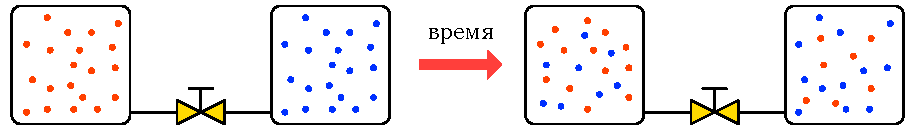
\includegraphics[width=\linewidth]{figs/entropy/gas_diffusion.pdf}
    \caption{Самопроизвольное смешивание газов.}
    \label{fig:gas_diffusion}
\end{figure}

Общая энергия системы здесь, как и в первом случае, не изменилась. Теплота не подводилась ($Q = 0$), работа над окружением не совершалась ($W = 0$), потому что суммарный объём остался прежним. Внутренняя энергия та же самая. Общее давление в системе тоже осталось прежним.

Несмотря на всё это, обратно газы сами не разделятся, хотя закон сохранения энергии и здесь этого не запрещает. Зададим те же самые вопросы:

\begin{itemize}
    \item в чём принципиальное различие этих состояний, если энергия не изменилась?
    \item откуда взялась <<движущая сила>>, заставившая газы смешаться?
\end{itemize}

С имеющимися до этого момента знаниями ответить на эти вопросы мы не сможем. Нам придётся изучить ещё одно новое свойство системы~--- \emph{энтроп\'{и}ю}.

\subsection*{Идея энтропии}

Если говорить простыми словами, \term{энтропия}{entropy}{энтропия} отвечает на следующий вопрос: \emph{сколькими разными способами может быть устроено данное состояние изнутри}. Давайте рассмотрим простую аналогию. У нас имеются две игральные кости, которые мы бросаем и смотрим на сумму выпавших чисел.

Сумму чисел, которую мы получаем при броске, назовём \term{макросостоянием}{macrostate}{макросостояние}. Выпавшие числа (например, на первой кости 3, на второй 4)~--- это один из вариантов того, как общая сумма могла получиться; назовём это \term{микросостоянием}{microstate}{микросостояние}.

Допустим, одна из костей белая, а другая красная~--- как это изображено в табл.~\ref{tab:dice}. Поэтому комбинации <<белая 3, красная 4>> и <<белая 4, красная 3>>~--- это два разных микросостояния, хотя макросостояние у них одно и то же.

Ни одна из граней костей ничем не выделена, поэтому каждое микросостояние равновероятно и выпадает с вероятностью $1/36$. А вот макросостояния равновероятными уже не будут.

\begin{table}[htbp]
    \small
    \caption{Макро- и микросостояния при бросании двух игральных костей: сумма~--- это макросостояние, $\Omega$~--- число отвечающих ему микросостояний.}
    \label{tab:dice}
    \begin{tabularx}{\textwidth}{
        >{\hsize=0.35\hsize}Z
        >{\hsize=0.40\hsize}Z
        >{\hsize=2.25\hsize}Y
        }
        \hline
        \rowcolor{green!5}
        Сумма & $\Omega$ & Варианты (микросостояния) \\
        \hline
        2 & 1 & \dpair{1}{1} \\
        \hline
        3 & 2 & \dpair{1}{2}\enspace \dpair{2}{1} \\
        \hline
        4 & 3 & \dpair{1}{3}\enspace \dpair{3}{1}\enspace \dpair{2}{2} \\
        \hline
        5 & 4 & \dpair{1}{4}\enspace \dpair{4}{1}\enspace \dpair{2}{3}\enspace \dpair{3}{2} \\
        \hline
        6 & 5 & \dpair{1}{5}\enspace \dpair{5}{1}\enspace \dpair{2}{4}\enspace \dpair{4}{2}\enspace \dpair{3}{3} \\
        \hline
        7 & 6 & \dpair{1}{6}\enspace \dpair{6}{1}\enspace \dpair{2}{5}\enspace \dpair{5}{2}\enspace \dpair{3}{4}\enspace \dpair{4}{3} \\
        \hline
        8 & 5 & \dpair{2}{6}\enspace \dpair{6}{2}\enspace \dpair{3}{5}\enspace \dpair{5}{3}\enspace \dpair{4}{4} \\
        \hline
        9 & 4 & \dpair{3}{6}\enspace \dpair{6}{3}\enspace \dpair{4}{5}\enspace \dpair{5}{4} \\
        \hline
        10 & 3 & \dpair{4}{6}\enspace \dpair{6}{4}\enspace \dpair{5}{5} \\
        \hline
        11 & 2 & \dpair{5}{6}\enspace \dpair{6}{5} \\
        \hline
        12 & 1 & \dpair{6}{6} \\
        \hline
    \end{tabularx}
\end{table}

Оказывается, что шансы выпадения разных сумм (то есть нахождения в определённых макросостояниях) неодинаковы. Вероятность выпадения 7 в шесть раз больше, чем 2.

При этом не существует никакой <<силы>>, которая бы стремилась к выпадению семёрки. Просто микросостояний, отвечающих ей, шесть, а способов получить двойку в качестве макросостояния~--- только один. Число микросостояний, отвечающих одному макросостоянию, называют его \term{статистическим весом}{statistical_weight}{статистический вес} и обозначают $\Omega$\footnote{Также эту величину называют \emph{термодинамической вероятностью}. Но не путайте её с обычной вероятностью! $\Omega$~--- это число вариантов, а не доля от единицы. Частенько статистический вес обозначают буквой $W$ (от нем. \emph{Wahrscheinlichkeit}~--- вероятность), однако в этой книге эта буква обозначает работу.}.

\subsection*{От двух костей к молю вещества}

У такой простой системы, как пара игральных костей, разница вероятностей выпадения разных состояний невелика~--- максимум шесть к одному. Двойка выпадает не так часто, но всё-таки в среднем один раз из 36 бросков она выпадет.

Теперь перенесёмся в волшебный мир больших чисел, касающихся описания вещества. Возьмём сосуд с газом, мысленно разделим его пополам и спросим: какова вероятность застать все молекулы в заранее выбранной половине? Если мы возьмём одну молекулу, то вероятность не такая уж и маленькая~--- $1/2$ (либо в одной половине, либо в другой). Однако вероятность того, что $N$ молекул \emph{одновременно} окажутся в одной половине, уже $1/2^N$. Далее масштабируем:

\begin{itemize}
    \item для $N = 10$: примерно один шанс из тысячи~--- даже выше, чем сорвать джекпот в лотерее;
    \item для $N = 100$: примерно $10^{-30}$;
    \item для $N = 6\cdot10^{23}$ (один моль): примерно $10^{-1{,}8\cdot 10^{23}}$.
\end{itemize}

Уже для сотни молекул такое событие практически невозможно: даже если бы такой эксперимент повторялся каждую секунду с самого начала существования Вселенной, шанс увидеть его хотя бы один раз остался бы неотличим от нуля. Для целого моля вещества слово <<невозможно>> перестаёт быть преувеличением и становится фактом\footnote{Тем не менее, для очень малых систем отклонения всё же наблюдаются. Вспомните, например, броуновское движение.}.

В итоге, для невероятно большого числа частиц, с которым мы имеем дело даже при рассмотрении 1 моля вещества, макросостояние с наибольшим статистическим весом настолько подавляет все остальные, что отклонений от него мы фактически не наблюдаем и формулируем это как закон природы.

Теперь мы можем ответить на вопрос о <<движущей силе>>, которая заставляет смешиваться газы и равномерно распределять тепло в системе~--- её не существует. Система на самом деле никуда не <<стремится>>~--- она просто с поражающей воображение вероятностью оказывается в том макросостоянии, которому отвечает наибольшее количество микросостояний (больший статистический вес).

\subsection*{Микросостояния вещества}

Вернёмся к рассмотрению веществ. Что такое микросостояние для вещества? Чтобы описать такое микросостояние, мы должны ответить на два вопроса: как распределена энергия между частицами и где они находятся. Поэтому для описания процессов удобно выделить два семейства микросостояний, так называемые энергетические конфигурационные (табл.~\ref{tab:microstates}). Впрочем, помните, что деление это условно~--- во многих процессах меняются оба вклада сразу.

\begin{table}[htbp]
    \small
    \caption{Два семейства микросостояний.}
    \label{tab:microstates}
    \begin{tabularx}{\textwidth}{
        >{\hsize=0.8\hsize}Y
        >{\hsize=1.1\hsize}Y
        >{\hsize=1.1\hsize}Y
        }
        \hline
        \rowcolor{green!5}
        Признак & Энергетические микросостояния & Конфигурационные микросостояния \\
        \hline
        Варианты чего & Как энергия распределена между частицами и степенями свободы & Где находятся частицы и какого они сорта \\
        \hline
        За счёт чего растёт число микросостояний & Энергии больше или уровни энергии расположены теснее~--- больше способов разложить её на кванты & Больше доступный объём или больше сортов частиц~--- больше способов расставить частицы \\
        \hline
        Чем обычно вызвано & Потоком теплоты или рассеянием работы (трение, вязкость) & Изменением объёма, состава или перемешиванием \\
        \hline
        Примеры & Нагревание, теплопроводность, трение, горение & Расширение, смешивание, диффузия, растворение \\
        \hline
    \end{tabularx}
\end{table}

Обратите внимание, что теплота~--- самый распространённый, но не единственный способ увеличить число энергетических микросостояний. Работа, потраченная на трение или вязкое сопротивление, делает то же самое, при этом вообще не пересекая границы системы. Например, мешалка (магнитная) будет нагревать жидкость в теплоизолированном сосуде, хотя теплообмена с окружением нет.

Как и в случае с игральными костями, все микросостояния, отвечающие данному состоянию системы, имеют равную вероятность. Это исходное допущение статистической физики, играющее ту же роль, что и честность игральных костей. Природа не <<предпочитает>> ни одно из них. Разница между макросостояниями только в том, что одним из них отвечает большее число микросостояний, чем другим\footnote{Заметьте, что в ситуации со смешением газов важно, что газы~А и~Б \emph{разные}. Если соединить два сосуда с одним и тем же газом, то после открытия крана система будет неотличима от исходной, поскольку частицы одного сорта неразличимы, новых вариантов расстановки не появляется, и энтропия не вырастет.}.

\subsection*{Фазовое пространство}

Чтобы полностью описать состояние одной частицы в механике, нам нужно знать, где она находится и как движется. Для частицы на прямой это можно сделать при помощи двух чисел~--- координаты и импульса. Для трёхмерного пространства таких чисел нужно уже шесть: три координаты и три проекции импульса. Для системы из $N$ частиц нужно $6N$ чисел, что для одного моля вещества составляет около $3{,}6\cdot10^{24}$ чисел.

\term{Фазовое пространство}{phase_space}{фазовое пространство}~--- это воображаемое пространство, у которого столько же осей, сколько чисел необходимо для определения состояния частиц. Одна точка в фазовом пространстве задаёт сразу все $3{,}6\cdot10^{24}$ чисел, то есть описывает систему полностью (у нас есть вся информация про каждую молекулу). То есть одна точка фазового пространства~--- это одно микросостояние.

Само фазовое пространство системы не меняется и не растёт. Однако представьте, что перед нами стакан воды, имеющий температуру \qty{20}{\degreeCelsius} (рис.~\ref{fig:phase_space}). Этому макросостоянию отвечает не одна точка, а некоторая \emph{область} фазового пространства~--- совокупность всех микросостояний, при нахождении в которых система имеет именно такую температуру. Эти микросостояния неразличимы по любым измеримым величинам. Число микросостояний в этой области и есть описанный выше статистический вес $\Omega$\footnote{В классическом описании точек в области бесконечно много, поэтому <<сосчитать>> микросостояния можно, только договорившись о размере ячейки. Последовательно это делает квантовая механика: там уровни энергии дискретны и микросостояния действительно можно сосчитать. Именно поэтому выше речь шла о способах разложить энергию на кванты.}.

\begin{figure}[htbp]
    \centering
    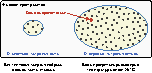
\includegraphics[width=10cm]{figs/entropy/phase_space.pdf}
    \caption{Как соотносятся фазовое пространство, макросостояние и микросостояние.}
    \label{fig:phase_space}
\end{figure}

Поэтому \emph{чем больше область фазового пространства, доступная системе в данном макросостоянии, тем больше статистический вес и тем больше энтропия}.

\subsection*{Почему нельзя использовать статистический вес непосредственно как энтропию}

Казалось бы, почему не использовать в качестве энтропии само число $\Omega$? Давайте рассмотрим на примере.

У нас имеются две системы. Давайте соединим их в одну. Каждое микросостояние первой сочетается с любым микросостоянием второй, поэтому статистические веса \emph{перемножаются}: $\Omega = \Omega_1 \Omega_2$. Аналогия для двух пар игральных костей будет представлять собой $36 \cdot 36 = 1296$ вариантов.

При этом энтропия должна вести себя как масса или энергия, то есть энтропия целого должна быть равна \emph{сумме} энтропий частей. Поэтому умножение нужно превратить в сложение, чего можно добиться, использовав свойства функции логарифма. Для энтропии используется определение, данное Больцманом:

\begin{equation*}
    S = k \ln \Omega,
\end{equation*}

где $k$~--- постоянная Больцмана. $\ln (\Omega_1 \Omega_2) = \ln \Omega_1 + \ln \Omega_2$, то есть энтропия системы равна сумме энтропий составляющих её частей. Также логарифм позволяет перейти от огромных статистических весов макроскопических систем к вполне обычным удобным числам.

Обратите внимание, что если состояние системы можно устроить ровно одним способом ($\Omega = 1$), то энтропия такой системы равна нулю ($S = k \ln 1 = 0$).

\subsection*{Возвращаемся к двум ситуациям}

Теперь мы можем вернуться в начало раздела и дать исчерпывающие ответы на поставленные нами вопросы.

\emph{Ситуация первая.} Суммарная энергия системы (предмета и комнаты) не изменилась, но после теплопередачи она оказалась распределена по-другому. Пока предмет горячий, а комната холодная, энергия сосредоточена в относительно небольшой части системы, и способов так её разложить по микросостояниям сравнительно немного. Когда температуры сравнялись, та же энергия оказывается распределена по всем частицам предмета и комнаты, и число способов сделать это максимально. Начальное и конечное состояния различаются числом энергетических микросостояний и, соответственно, объёмом доступного фазового пространства. Энтропия связки система + окружение растёт.

\emph{Ситуация вторая.} Общая энергия также не изменилась, но каждой молекуле газа~А стал доступен вдвое больший объём, и то же самое произошло с газом~Б. Число способов расставить частицы выросло для каждого газа в $2^{\num{6,02e23}}$ раз\footnote{Объём удваивается, поэтому число доступных положений возрасло вдвое. Поскольку молекулы независимы, для $N$ молекул число способов перемножается: $2 \cdot 2 \cdot \ldots \cdot 2 = 2^N$. Для одного моля $N = \num{6,02e23}$, откуда получаем $2^{\num{6,02e23}}$.}, то есть примерно в $10^{\num{1,8e23}}$ раз. Число доступных микросостояний (конфигурационных) снова выросло, а с ним и энтропия.

Таким образом, чтобы процесс был самопроизвольным, \emph{общее изменение энтропии} $\Delta S_{\text{общ}} = \Delta S_{\text{сист}} + \Delta S_{\text{окр}}$ \emph{должно быть положительным}. При этом локально энтропия как системы, так и окружения может уменьшаться, но в целом для связки система + окружение она всегда увеличивается (или, по крайней мере, не изменяется). Это правило называют \term{вторым законом термодинамики}{second_law_of_thermodynamics}{второй закон термодинамики}.

Второй закон термодинамики определяет \emph{фундаментальную возможность или невозможность процессов} (в том числе и химических реакций)\footnote{При этом, будет ли процесс происходить на самом деле, ещё неизвестно. Определяется сам факт принципиальной возможности.}. Из его математического вида также становится понятно, почему химическую реакцию не имеет смысла рассматривать без учёта окружения, в котором она находится, поскольку уменьшение энтропии самой реагирующей системы вовсе не означает, что реакция невозможна, просто при этом энтропия окружения возрастает ещё сильнее.

\subsection*{Как оценить энтропию на глаз}

Если поискать в интернете определение энтропии, то первое, на что вы наткнётесь, это достаточно бытовое определение энтропии как меры беспорядка, хаоса. На этой основе зачастую стремятся обозначить некоторые правила, которые позволяют <<на глаз>> определить, растёт энтропия в том или ином процессе или нет. Зачастую это работает, однако такой подход довольно поверхностный. Хороший химик должен оперировать научными критериями оценки энтропии, а именно~--- увеличением или уменьшением доступного фазового пространства. Используя качественные подходы, легко ошибиться, и вы всегда должны помнить об этом.

Тем не менее, для общей эрудиции мы должны упомянуть, как можно оценить изменение энтропии в процессе.

\begin{itemize}
    \item Агрегатные состояния обладают возрастающей энтропией в порядке: $S_{\text{тв}}$ < $S_{\text{ж}}$ < $S_{\text{г}}$. Рост энтропии при плавлении связан с появлением у частиц поступательных степеней свободы (они перестают быть жёстко закреплены в узлах решётки), а при кипении~--- с многократным увеличением доступного объёма на частицу и исчезновением ближнего порядка. Энтропия идеального газа растёт при изотермическом расширении, тогда как внутренняя энергия при этом не меняется.
    \item Более организованное вещество обладает меньшей энтропией, чем менее организованное. Например, изменение энтропии в процессе растворения веществ, как правило, положительно из-за энтропии смешения (конфигурационной энтропии) и появления у частиц поступательных степеней свободы в объёме раствора. Выполняется это не всегда. Например, при растворении \ce{NaCl} энтропия действительно растёт, а при растворении \ce{MgCl2}~--- уменьшается. Компактный двухзарядный катион магния создаёт плотную шубу из ориентированных молекул воды (электрострикция), уменьшая энтропию окружения больше, чем она увеличивается за счёт разрушения кристалла соли.
    \item Реакции, увеличивающие число частиц в системе, \emph{как правило}, увеличивают энтропию этой системы. В конце такой реакции увеличивается количество доступных микросостояний, и сама система теперь внутренне более неупорядочена, поскольку содержит больше компонентов. Впрочем, это почти всегда верно для газообразных веществ, однако часто не выполняется для жидкостей и твёрдых тел.
\end{itemize}

\begin{termlist}
    \hyperref[term:entropy]{Энтропия},
    \hyperref[term:macrostate]{макросостояние},
    \hyperref[term:microstate]{микросостояние},
    \hyperref[term:statistical_weight]{статистический вес},
    \hyperref[term:phase_space]{фазовое пространство},
    \hyperref[term:second_law_of_thermodynamics]{второй закон термодинамики}.
\end{termlist}

\clearpage

\section{Энтропия в химических реакциях}

Теперь давайте обсудим, как происходит изменение энтропии в химических реакциях. Согласно \hyperref[term:second_law_of_thermodynamics]{второму закону термодинамики}, для самопроизвольных процессов (к которым, разумеется, относятся многие химические реакции) \emph{сумма изменений энтропии реагирующей системы и окружения должна быть положительна}:

\begin{equation*}
    \boxed{\Delta S_{\text{общ}} = \Delta S_{\text{сист}} + \Delta S_{\text{окр}} > 0}.
\end{equation*}

При этом вовсе не обязательно, чтобы росла энтропия реагирующей системы, важно только, чтобы росла общая сумма. Поэтому реакции, сопровождающиеся уменьшением энтропии реагирующей системы, вполне возможны.

Изменение энтропии реагирующей системы складывается из двух вкладов, которые мы \hyperref[tab:microstates]{обсуждали} в предыдущем разделе: энергетический (как энергия распределена между частицами и степенями свободы) и конфигурационный (где находятся частицы и какого они сорта):

\begin{equation*}
    \boxed{\Delta S_{\text{сист}} = \Delta S_{\text{энерг}} + \Delta S_{\text{конф}}}.
\end{equation*}

Для окружения изменяется только $\Delta S_{\text{энерг}}$, потому что мы рассматриваем частицы реагирующего вещества отдельно от окружения (по большей части, нам про него ничего не известно). По сути, окружение можно рассматривать как \emph{огромный термостат}, способный принять или отдать любое количество энергии.

\subsection*{Связь энтропии и энтальпии}

$\Delta S_{\text{энерг}}$ определить сравнительно легко (правда, только для окружения), так как она зависит от количества переданной энергии:

\begin{equation*}
    \Delta S_{\text{энерг}} = \frac{Q}{T},
\end{equation*}

где $\Delta S_{\text{энерг}}$~--- изменение энтропии тела (энергетическая составляющая), $Q$~--- количество теплоты, полученной этим телом, $T$~--- температура.

Получение объектом энергии увеличивает его энтропию за счёт энергетических микросостояний, потому что становится больше способов разложить энергию на кванты.

Поэтому если при протекании химической реакции энергия передаётся системе (реакция эндотермическая), то вклад $\Delta S_{\text{энерг}}$ в энтропию реагирующей системы положителен. Если наоборот~--- энергия уходит из системы и передаётся окружению, то $\Delta S_{\text{энерг}}$ системы будет отрицательным.

Применим эту формулу к окружению. Для него меняется только энергетическая составляющая энтропии, а процесс передачи энергии можно представить как обратимый изотермический процесс. Сколько теплоты система отдала, столько окружение и получило, поэтому при постоянном давлении $Q_{\text{окр}} = -\Delta H$, где $\Delta H$~--- энтальпия реакции, то есть величина, относящаяся к \emph{системе}. Отсюда

\begin{equation}
    \label{eq:entropy_of_the_surroundings}
    \boxed{\Delta S_{\text{окр}} = \frac{Q_{\text{окр}}}{T} = -\frac{\Delta H}{T}}.
\end{equation}

Знак минус здесь означает ровно то, что мы уже сказали словами: экзотермическая реакция ($\Delta H < 0$) отдаёт энергию окружению и увеличивает его энтропию, а эндотермическая ($\Delta H > 0$)~--- забирает энергию и уменьшает (рис.~\ref{fig:entropy_balance}).

\begin{figure}[htbp]
    \centering
    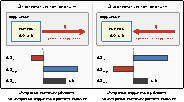
\includegraphics[width=\linewidth]{figs/entropy_in_chemical_reactions/entropy_balance.pdf}
    \caption{Почему реакция может идти при убывающей энтропии системы.}
    \label{fig:entropy_balance}
\end{figure}

Соответственно, единицами измерения $\Delta S$ будут

\begin{equation*}
    [\Delta S] = \frac{[Q]}{[T]} = \frac{\unit{\ruJ}}{\unit{\ruK}}.
\end{equation*}

Например, окружению при \qty{298}{\ruK} было передано \qty{100}{\ruKJ} теплоты, значит, его энтропия возрастёт на

\begin{equation*}
    \Delta S_{\text{окр}} = \frac{\num{100}}{\num{298}} = \qty{0,336}{\ruKJ\per\ruK} = \qty{336}{\ruJ\per\ruK}.
\end{equation*}

Для химических реакций обычно используют мольные величины: \unit{\ruJ\per\ruK\ruMole}.

Заманчиво применить ту же формулу и к самой реагирующей системе, однако запись $\Delta S_{\text{сист}} = \Delta H/T$ неверна по двум причинам:

\begin{itemize}
    \item кроме $\Delta S_{\text{энерг}}$ существует также вклад $\Delta S_{\text{конф}}$;
    \item в ходе реакции меняется сама природа частиц (то есть сами энергетические уровни), поэтому для реагирующей системы $\Delta S_{\text{энерг}} \neq \frac{\Delta H}{T}$.
\end{itemize}

Для реагирующей системы изменение $\Delta S_{\text{сист}}$ \emph{нужно рассчитывать по справочным данным} на основании \hyperref[term:law_of_Hess]{закона Гесса} (поскольку энтропия является функцией состояния).

\begin{example}{}{entropy_in_chemical_reactions1}
    \begin{condition}
        Почему реакция
        \reaction*{H2_{\textup{(г)}} + \frac{1}{2}O2_{\textup{(г)}} -> H2O_{\textup{(г)}}}
        идёт самопроизвольно, если $\Delta S_{\textup{сист}}$ для этой реакции отрицательна: \qty{-44,5}{\ruJ\per\ruK\ruMole}?
    \end{condition}

    \medskip

    \textit{Решение.} Рассматривая только изменение энтропии системы, нам может показаться, что реакция не будет самопроизвольной. Однако это не так. Реакция кислорода с водородом происходит со взрывом, при этом от системы к окружению передаётся огромное количество энергии: энтальпия этой реакции равна \qty{-241,82}{\ruKJ\per\ruMole}. По формуле~\eqref{eq:entropy_of_the_surroundings} при \qty{298}{\ruK} получаем
    \begin{equation*}
        \Delta S_{\text{окр}} = -\frac{\Delta H}{T} = -\frac{\num{-241820}}{\num{298}} = \qty{811,5}{\ruJ\per\ruK\ruMole},
    \end{equation*}
    то есть на самом деле $\Delta S_{\text{окр}}$ имеет большое положительное значение.

    Член $\Delta S_{\text{окр}}$ настолько велик, что компенсирует отрицательное значение $\Delta S_{\text{сист}}$ и $\Delta S_{\text{общ}}$ становится положительным:
    \begin{equation*}
        \Delta S_{\text{общ}} = \Delta S_{\text{сист}} + \Delta S_{\text{окр}} = \num{-44,5} + \num{811,5} = \qty{767}{\ruJ\per\ruK\ruMole}.
    \end{equation*}
    Поэтому эта реакция самопроизвольна.
\end{example}

\subsection*{Связь энтропии и температуры}

Как вы можете видеть из формулы~\eqref{eq:entropy_of_the_surroundings}, изменение энтропии зависит ещё и от температуры~--- при более низких температурах энтропия меняется сильнее при передаче того же количества теплоты. Это происходит потому, что энтропия оценивает не абсолютное количество переданной энергии, а то, насколько сильно эта энергия меняет доступный объём фазового пространства системы на её текущем уровне:

\begin{itemize}
    \item При низких температурах тепловой энергии мало, и частицы находятся на низких энергетических уровнях, поэтому число доступных микросостояний $\Omega$ относительно невелико. Если передать такой системе некоторое количество теплоты, то эта энергия откроет частицам доступ к множеству новых, ранее недоступных уровней, из-за чего число способов распределить энергию станет многократно больше.
    \item При высоких температурах частицы уже обладают большой энергией и заселяют большое количество энергетических уровней (доступный объём фазового пространства уже большой). Добавление того же количества теплоты откроет незначительное количество новых микросостояний.
\end{itemize}

Простая аналогия этого~--- вы чихаете в библиотеке, отчего возникает большой относительный беспорядок. Либо вы чихаете в метро, где среди общего шума это будет практически незаметно.

Зависимость энтропии окружения от температуры ($\Delta S_{\text{окр}} = -\frac{\Delta H}{T}$) означает, что вклад теплового эффекта в общую движущую силу реакции меняется с температурой. При низких температурах этот вклад огромен (реакция идёт за счёт выделения тепла), а при высоких~--- становится незначительным (рис.~\ref{fig:entropy_and_temperature}), и главную роль начинает играть изменение энтропии самой системы ($\Delta S_{\text{сист}}$).

\begin{figure}[htbp]
    \centering
    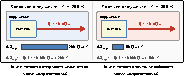
\includegraphics[width=\linewidth]{figs/entropy_in_chemical_reactions/entropy_and_temperature.pdf}
    \caption{Относительный вклад теплоты в энтропию зависит от температуры.}
    \label{fig:entropy_and_temperature}
\end{figure}

\begin{example}{}{entropy_in_chemical_reactions2}
    \begin{condition}
        Почему вода замерзает при температурах ниже нуля, а не при более высоких?
    \end{condition}

    \medskip

    \textit{Решение.} Изменение энтропии ($\Delta S_{\text{сист}}$) при фазовом превращении
    \reaction*{H2O_{\text{(ж)}} -> H2O_{\text{(тв)}}}
    находим из справочных данных: \qty{-22,0}{\ruJ\per\ruK\ruMole}.

    $\Delta S_{\text{окр}}$ \hyperref[eq:entropy_of_the_surroundings]{зависит от температуры}, рассчитаем его при \qty{-10}{\degreeCelsius} и при \qty{10}{\degreeCelsius} (\num{263} и \qty{283}{\ruK}). Энтальпию процесса \ce{H2O_{\text{(ж)}} -> H2O_{\text{(тв)}}} найдём из справочных данных по закону Гесса: \qty{-6010}{\ruJ\per\ruMole}.

    При \qty{10}{\degreeCelsius}:
    \begin{equation*}
        \Delta S_{\text{окр}} = -\frac{\Delta H}{T} = -\frac{\num{-6010}}{\num{283}} = \qty{21,2}{\ruJ\per\ruK\ruMole}.
    \end{equation*}
    При \qty{-10}{\degreeCelsius}:
    \begin{equation*}
        \Delta S_{\text{окр}} = -\frac{\Delta H}{T} = -\frac{\num{-6010}}{\num{263}} = \qty{22,9}{\ruJ\per\ruK\ruMole}.
    \end{equation*}
    Теперь рассчитываем $\Delta S_{\text{общ}}$ при обеих температурах:

    При \qty{10}{\degreeCelsius}:
    \begin{equation*}
        \Delta S_{\text{общ}} = \Delta S_{\text{сист}} + \Delta S_{\text{окр}} = \num{-22,0} + \num{21,2} = \qty{-0,8}{\ruJ\per\ruK\ruMole}.
    \end{equation*}

    При \qty{-10}{\degreeCelsius}:
    \begin{equation*}
        \Delta S_{\text{общ}} = \Delta S_{\text{сист}} + \Delta S_{\text{окр}} = \num{-22,0} + \num{22,9} = \qty{0,9}{\ruJ\per\ruK\ruMole}.
    \end{equation*}
    Самопроизвольность замерзания воды при отрицательных температурах обусловлена общим возрастанием энтропии системы + окружения в этом случае.
\end{example}

\begin{problem}{}{entropy_in_chemical_reactions1}
    Промышленный синтез аммиака идёт по уравнению
    \reaction*{N2_{(\text{г})} + 3H2_{(\text{г})} -> 2NH3_{(\text{г})}{.}}
    Рассчитайте $\Delta S_{\text{сист}}$, $\Delta S_{\text{окр}}$ и $\Delta S_{\text{общ}}$ при \qty{298}{\ruK} и определите, самопроизвольна ли реакция. Стандартные энтропии $S^{\circ}$, \unit{\ruJ\per\ruK\ruMole}: \ce{N2} \num{191,6}, \ce{H2} \num{130,7}, \ce{NH3} \num{192,8} (все вещества газообразные). Стандартная теплота образования $\Delta{}_fH^{\circ}(\ce{NH3}, \text{г}) = \qty{-45,9}{\ruKJ\per\ruMole}$.
    \begin{sol}{\ref{prob:entropy_in_chemical_reactions1}}
        Энтропия~--- функция состояния, поэтому её изменение рассчитывается по закону Гесса: сумма по продуктам минус сумма по исходным веществам, с учётом коэффициентов:
        \begin{equation*}
            \Delta S_{\text{сист}} = 2 \cdot \num{192,8} - \num{191,6} - 3 \cdot \num{130,7} = \qty{-198,1}{\ruJ\per\ruK\ruMole}.
        \end{equation*}

        Обратите внимание, что здесь логично убывание энтропии в реакции, потому что из четырёх молей газа получается два, доступный объём фазового пространства уменьшается.

        Тепловой эффект тоже рассчитываем по закону Гесса (теплоты образования простых веществ равны нулю): $\Delta H = 2 \cdot (\num{-45,9}) = \qty{-91,8}{\ruKJ\per\ruMole}$. Тогда
        \begin{equation*}
            \Delta S_{\text{окр}} = -\frac{\Delta H}{T} = -\frac{\num{-91800}}{\num{298}} = \qty{308,1}{\ruJ\per\ruK\ruMole},
        \end{equation*}
        \begin{equation*}
            \Delta S_{\text{общ}} = \num{-198,1} + \num{308,1} = \qty{110,0}{\ruJ\per\ruK\ruMole} > 0.
        \end{equation*}

        Таким образом, реакция самопроизвольна при \qty{298}{\ruK}, хотя энтропия самой реагирующей системы уменьшается. Тем не менее выделяющаяся теплота увеличивает энтропию окружения сильнее, чем система теряет свою.
    \end{sol}
\end{problem}

\begin{problem}{}{entropy_in_chemical_reactions2}
    Получение извести обжигом известняка соответствует реакции:
    \reaction*{CaCO3_{(\text{тв})} -> CaO_{(\text{тв})} + CO2_{(\text{г})}{.}}
    Покажите, что при \qty{298}{\ruK} этот процесс не самопроизвольный, и найдите температуру, выше которой он становится самопроизвольным. Считайте, что $\Delta H$ и $\Delta S_{\text{сист}}$ от температуры не зависят. Стандартные теплоты образования $\Delta{}_fH^{\circ}$, \unit{\ruKJ\per\ruMole}: \ce{CaCO3} \num{-1207,6}, \ce{CaO} \num{-634,9}, \ce{CO2} \num{-393,5}. Стандартные энтропии $S^{\circ}$, \unit{\ruJ\per\ruK\ruMole}: \ce{CaCO3} \num{91,7}, \ce{CaO} \num{38,1}, \ce{CO2} \num{213,8}.
    \begin{sol}{\ref{prob:entropy_in_chemical_reactions2}}
        По закону Гесса:
        \begin{equation*}
            \Delta H = (\num{-634,9} - \num{393,5}) - (\num{-1207,6}) = \qty{179,2}{\ruKJ\per\ruMole},
        \end{equation*}
        \begin{equation*}
            \Delta S_{\text{сист}} = \num{38,1} + \num{213,8} - \num{91,7} = \qty{160,2}{\ruJ\per\ruK\ruMole}.
        \end{equation*}

        Реакция эндотермическая, но энтропия системы растёт (потому что из твёрдого вещества выделяется газ). Имеем два противоположных вклада и то, будет ли реакция самопроизвольной, определяет температура.

        При \qty{298}{\ruK}:
        \begin{equation*}
            \Delta S_{\text{окр}} = -\frac{\num{179200}}{\num{298}} = \qty{-601,3}{\ruJ\per\ruK\ruMole},
        \end{equation*}
        \begin{equation*}
            \Delta S_{\text{общ}} = \num{160,2} - \num{601,3} = \qty{-441,1}{\ruJ\per\ruK\ruMole} < 0,
        \end{equation*}
        то есть при комнатной температуре известняк устойчив.

        \emph{Граница самопроизвольности}~--- температура, при которой $\Delta S_{\text{общ}}$ обращается в ноль:
        \begin{equation*}
            \num{160,2} - \frac{\num{179200}}{T} = 0, \qquad T = \frac{\num{179200}}{\num{160,2}} \approx \qty{1119}{\ruK} \approx \qty{846}{\degreeCelsius}.
        \end{equation*}

        Выше этой температуры член $-\Delta H/T$ становится достаточно мал, чтобы рост энтропии системы его перекрыл. Реальные обжиговые печи работают при \num{900}--\qty{1000}{\degreeCelsius} чтобы обечпечить некоторый запас над расчётным значением температуры.
    \end{sol}
\end{problem}

\begin{problem}{}{entropy_in_chemical_reactions3}
    Профессор Недоумелкин рассуждает так: <<Из формулы~\eqref{eq:entropy_of_the_surroundings} видно, что с ростом температуры вклад $\Delta S_{\text{окр}}$ стремится к нулю. Значит, при очень высоких температурах все эндотермические реакции становятся самопроизвольными, а все экзотермические~--- перестают идти>>. Верно ли это? Если нет, то в чём ошибка? Перечислите все возможные случаи.
    \begin{sol}{\ref{prob:entropy_in_chemical_reactions3}}
        Первая половина этого вывода верна, вторая~--- нет. Верно, что при $T \to \infty$ член $-\Delta H/T$ стремится к нулю и знак $\Delta S_{\text{общ}}$ определяется знаком одного лишь $\Delta S_{\text{сист}}$. Ошибка~--- в допущении, будто у эндотермических реакций $\Delta S_{\text{сист}} > 0$, а у экзотермических $\Delta S_{\text{сист}} < 0$. Никакой связи между знаками $\Delta H$ и $\Delta S_{\text{сист}}$ нет. Это независимые величины, и возможны перечисленные ниже четыре сочетания.

        \begin{enumerate}[label=\arabic*)]
            \item $\Delta H < 0$, $\Delta S_{\text{сист}} > 0$. Оба слагаемых положительны, реакция самопроизвольна при любой температуре. Пример~--- разложение пероксида водорода \ce{2H2O2_{(\text{ж})} -> 2H2O_{(\text{ж})} + O2_{(\text{г})}}: $\Delta H = \qty{-196}{\ruKJ\per\ruMole}$, $\Delta S_{\text{сист}} = +\qty{126}{\ruJ\per\ruK\ruMole}$.
            \item $\Delta H < 0$, $\Delta S_{\text{сист}} < 0$. При низких температурах реакция самопроизвольна, выше некоторой температуры~--- нет. Пример~--- синтез аммиака из задачи~\ref{prob:entropy_in_chemical_reactions1}.
            \item $\Delta H > 0$, $\Delta S_{\text{сист}} > 0$. Наоборот: реакция не идёт при низких температурах, но становится самопроизвольной выше некоторой. Пример~--- обжиг известняка из задачи~\ref{prob:entropy_in_chemical_reactions2}.
            \item $\Delta H > 0$, $\Delta S_{\text{сист}} < 0$. Оба слагаемых отрицательны, и реакция не идёт ни при какой температуре. Пример~--- получение озона из кислорода \ce{3O2_{(\text{г})} -> 2O3_{(\text{г})}}: $\Delta H = +\qty{285}{\ruKJ\per\ruMole}$, $\Delta S_{\text{сист}} = \qty{-138}{\ruJ\per\ruK\ruMole}$. Озон получают не нагреванием, а подводя энергию к системе извне: электрическим разрядом или ультрафиолетом.
        \end{enumerate}

        Другими словами, температура <<выключает>> не экзотермические реакции, а зависимость исхода от теплового эффекта вообще: при высоких температурах судьбу реакции решает только $\Delta S_{\text{сист}}$, каким бы ни был знак $\Delta H$.

        Тем не менее помните, что рассуждение про $T \to \infty$ опирается на постоянство $\Delta H$ и $\Delta S_{\text{сист}}$, а они на самом деле сами зависят от температуры (кроме того, скорее всего задолго до <<бесконечной температуры>> вещества уже разложатся). Речь идёт о тенденции.
    \end{sol}
\end{problem}

\begin{problem}{}{entropy_in_chemical_reactions4}
    В этом разделе сказано, что для реагирующей системы запись $\Delta S_{\text{сист}} = \Delta H/T$ неверна. Возьмём, однако, испарение воды
    \reaction*{H2O_{(\text{ж})} -> H2O_{(\text{г})}}
    и применим её для двух температур:

    \begin{itemize}
        \item при \qty{373}{\ruK}, где $\Delta H_{\text{исп}} = \qty{40,7}{\ruKJ\per\ruMole}$, получаем $\num{40700}/\num{373} = \qty{109}{\ruJ\per\ruK\ruMole}$~--- это в точности справочное значение $\Delta S_{\text{сист}}$ для процесса кипения воды;
        \item при \qty{298}{\ruK}, где $\Delta H_{\text{исп}} = \qty{44,0}{\ruKJ\per\ruMole}$, получаем $\num{44000}/\num{298} = \qty{147,7}{\ruJ\per\ruK\ruMole}$, тогда как справочное значение для этой температуры $\Delta S_{\text{сист}} = \num{188,8} - \num{70,0} = \qty{118,8}{\ruJ\per\ruK\ruMole}$.
    \end{itemize}

    Почему в первом случае <<неверная>> формула дала точный ответ, а во втором~--- нет?
    \begin{sol}{\ref{prob:entropy_in_chemical_reactions4}}
        Совпадение при \qty{373}{\ruK} не имеет отношения к формуле $\Delta S_{\text{энерг}} = Q/T$ и получается по совсем другой причине. \qty{373}{\ruK}~--- температура, при которой жидкая вода и пар при давлении \qty{1}{\ruAtm} находятся в \emph{равновесии}. Равновесие означает, что процесс обратим, то есть $\Delta S_{\text{общ}} = 0$. А раз так,
        \begin{equation*}
            \Delta S_{\text{сист}} = -\Delta S_{\text{окр}} = \frac{\Delta H}{T}.
        \end{equation*}
        То есть это равенство ~--- следствие равновесия, и выполняется оно только при той единственной температуре, при которой процесс равновесен.

        А вот при \qty{298}{\ruK} вода и пар при \qty{1}{\ruAtm} не в равновесии (нет кипения),~--- поэтому $\Delta S_{\text{общ}} \neq 0$ и равенство не соблюдается. Второй расчёт показал то, что и должен,
        \begin{equation*}
            \Delta S_{\text{общ}} = \num{118,8} - \num{147,7} = \qty{-28,9}{\ruJ\per\ruK\ruMole} < 0,
        \end{equation*}
        то есть превращение воды в пар под давлением \qty{1}{\ruAtm} при \qty{298}{\ruK} не самопроизвольно.

        Тот же приём мы уже видели в примере~\ref{ex:entropy_in_chemical_reactions2}: при \qty{273}{\ruK}~--- равновесной температуре плавления~--- сумма $\Delta S_{\text{сист}} + \Delta S_{\text{окр}}$ обращается в нуль, а по разные стороны от неё меняет знак.
    \end{sol}
\end{problem}

\begin{problem}{}{entropy_in_chemical_reactions5}
    В спортивных аптечках встречается так называемый <<холодный пакет>>, внутри которого имеются вода и кристаллы нитрата аммония, разделённые перегородкой. Если сломать перегородку, соль растворяется, и пакет сильно охлаждается:
    \reaction*{NH4NO3_{(\text{тв})} -> NH4^+ + NO3^-{,}}
    причём для этого процесса $\Delta H = +\qty{25,7}{\ruKJ\per\ruMole}$. Тем не менее растворение идёт само.

    \begin{enumerate}[label=\arabic*)]
        \item Покажите расчётом, что при \qty{298}{\ruK} процесс самопроизволен.
        \item Оцените температуру, ниже которой он перестал бы быть самопроизвольным.
        \item Почему на практике эта граница недостижима?
    \end{enumerate}

    Данные. Стандартные энтропии $S^{\circ}$, \unit{\ruJ\per\ruK\ruMole}: \ce{NH4NO3} (тв.) \num{151,1}, \ce{NH4^+} (в растворе) \num{113,4}, \ce{NO3^-} (в растворе) \num{146,4}.
    \begin{sol}{\ref{prob:entropy_in_chemical_reactions5}}
        1)~Изменение энтропии системы должно быть положительным, поскольку кристаллическая решётка разрушается, ионы расходятся по всему объёму раствора, следовательно растёт конфигурационная составляющая энтропии:
        \begin{equation*}
            \Delta S_{\text{сист}} = \num{113,4} + \num{146,4} - \num{151,1} = +\qty{108,7}{\ruJ\per\ruK\ruMole}.
        \end{equation*}

        Окружение отдаёт теплоту, поэтому его энтропия падает:
        \begin{equation*}
            \Delta S_{\text{окр}} = -\frac{\num{25700}}{\num{298}} = \qty{-86,2}{\ruJ\per\ruK\ruMole},
        \end{equation*}
        \begin{equation*}
            \Delta S_{\text{общ}} = \num{108,7} - \num{86,2} = +\qty{22,5}{\ruJ\per\ruK\ruMole} > 0.
        \end{equation*}
        Таким образом, процесс самопроизволен, хотя окружение при этом теряет энтропию.

        2)~Чем ниже температура, тем дороже обходится отбор теплоты у окружения, потому что модуль $\Delta H/T$ растёт. Граница самопроизвольности будет там, где общее изменение энтропии станет равно нулю:
        \begin{equation*}
            \num{108,7} - \frac{\num{25700}}{T} = 0, \qquad T = \frac{\num{25700}}{\num{108,7}} \approx \qty{236}{\ruK} \approx \qty{-37}{\degreeCelsius}.
        \end{equation*}

        3)~При такой температуре вода замерзает и использовать её уже нельзя. Кроме того, расчёт опирался на постоянство $\Delta H$ и $\Delta S_{\text{сист}}$, а на интервале в шестьдесят градусов они заметно меняются. Поэтому значение температуры в \qty{-37}{\degreeCelsius} довольно условно. Тем не менее, это хорошо показывает, как холодное окружение <<сопротивляется>> отбору теплоты сильнее горячего.
    \end{sol}
\end{problem}

\begin{problem}{}{entropy_in_chemical_reactions6}
    В примере~\ref{ex:entropy_in_chemical_reactions1} значение $\Delta S_{\text{окр}}$ оказалось почти в 18 раз больше по модулю, чем $\Delta S_{\text{сист}}$. Чтобы почувствовать, насколько это много, вернитесь к формуле Больцмана $S = k \ln \Omega$ и оцените, во сколько раз увеличивается \emph{статистический вес} окружения, если передать ему \qty{100}{\ruKJ} теплоты при \qty{298}{\ruK}. Постоянная Больцмана $k = \qty{1,380649e-23}{\ruJ\per\ruK}$.
    \begin{sol}{\ref{prob:entropy_in_chemical_reactions6}}
        Прирост энтропии окружения нам уже известен: $\Delta S_{\text{окр}} = \num{100000}/\num{298} = \qty{335,6}{\ruJ\per\ruK}$. По формуле Больцмана
        \begin{equation*}
            \Delta S = k \ln \Omega_2 - k \ln \Omega_1 = k \ln \frac{\Omega_2}{\Omega_1},
        \end{equation*}
        откуда
        \begin{equation*}
            \ln \frac{\Omega_2}{\Omega_1} = \frac{\num{335,6}}{\num{1,380649e-23}} \approx \num{2,4e25}, \qquad
            \frac{\Omega_2}{\Omega_1} \approx e^{\num{2,4e25}} \approx 10^{\num{1,1e25}}.
        \end{equation*}

        Это число, у которого только в показателе степени двадцать пять разрядов. Чтобы вы поняли значение этих цифр: например, количество атомов в наблюдаемой Вселенной всего около $10^{80}$.

        Отсюда видно, почему в примере~\ref{ex:entropy_in_chemical_reactions1} член $\Delta S_{\text{окр}}$ так легко перекрыл убыль энтропии системы. За каждым джоулем, ушедшим в окружение, стоит астрономический рост числа доступных микросостояний, и <<небольшая>> на вид величина $-\Delta H/T$ на деле означает колоссальное изменение $\Omega$. Заодно понятно, зачем в определении энтропии стоит логарифм: без него сравнивать такие числа было бы крайне неудобно.
    \end{sol}
\end{problem}

\clearpage

\section[Откуда берётся новая энтропия. Энергия Гиббса]{Откуда берётся новая энтропия.\\Энергия Гиббса}

Мы уже знаем, что энтропия растёт при увеличении числа доступных микросостояний, то есть доступного объёма \hyperref[term:phase_space]{фазового пространства}. Если согласно \hyperref[term:second_law_of_thermodynamics]{второму закону термодинамики} энтропия связки система~+ окружение в самопроизвольных химических реакциях всегда возрастает, то возникает вопрос: откуда же берётся новая энтропия?

Существует два пути производства энтропии в реакциях, они отвечают двум вкладам, которые мы \hyperref[tab:microstates]{разбирали} ранее:

\begin{itemize}
    \item \term{Термализация}{thermalization}{термализация}~--- энергия, выделившаяся в ходе реакции, расходуется на тепловое движение частиц, а не на работу, которую можно использовать. Этот путь соответствует энергетическому вкладу в энтропию ($\Delta S_{\text{энерг}}$), причём в основном не системы, а окружения. Чтобы пойти по этому пути, реакция должна быть экзотермической, а количество произведённой энтропии быть больше, чем уменьшение энтропии реагирующей системы, если оно есть.
    \item Рост конфигурационного вклада в энтропию ($\Delta S_{\text{конф}}$). Обычно он связан с увеличением числа частиц, доступного объёма и тому подобным.
\end{itemize}

Чаще всего работают оба пути сразу, но один из них преобладает.

\subsection*{Энергия Гиббса}

Пользоваться условием $\Delta S_{\text{общ}} > 0$ напрямую неудобно, потому что оно требует каждый раз оценивать, что происходит и с системой, и с окружением. Но от рассмотрения окружения можно избавиться, анализируя только саму систему. Давайте рассмотрим, каким образом.

Пусть температура и давление постоянны, а система не совершает никакой работы, кроме работы расширения. Тогда изменение энтропии окружения определяется формулой~\eqref{eq:entropy_of_the_surroundings}, и условие самопроизвольности принимает вид

\begin{equation*}
    \Delta S_{\text{общ}} = \Delta S_{\text{сист}} + \Delta S_{\text{окр}} = \Delta S_{\text{сист}} - \frac{\Delta H}{T} > 0.
\end{equation*}

Умножим обе части на $-T$. Абсолютная температура величина всегда положительная, поэтому знак неравенства меняется на противоположный:

\begin{equation*}
    \Delta H - T \Delta S_{\text{сист}} < 0.
\end{equation*}

Слева у нас оказались только величины, определяющие свойства самой системы. Введём для неё отдельную функцию состояния

\begin{equation}
    \label{eq:gibbs_energy}
    \boxed{G = H - TS},
\end{equation}

которая называется \term{энергией Гиббса}{gibbs_energy}{энергия Гиббса}\footnote{Исторически её называли \emph{свободной энергией Гиббса}; это название до сих пор широко употребляется, и мы будем пользоваться обоими.}. Тогда условие самопроизвольности химической реакции можно записать так:

\begin{equation}
    \label{eq:gibbs_criterion}
    \boxed{\Delta G = \Delta H - T \Delta S_{\text{сист}} < 0}.
\end{equation}

Почему эту энергию называют \emph{свободной}? В чём физический смысл выражения~\eqref{eq:gibbs_criterion}?

Первый член~--- энтальпийный~--- определяет всю энергию, которую реакция способна отдать. Потратить её можно либо на совершение работы, либо на рост энтропии за счёт термализации.

Второй член~--- энтропийный~--- учитывает изменение энтропии самой системы. Если энтропия системы падает ($\Delta S_{\text{сист}} < 0$), то по \hyperref[term:second_law_of_thermodynamics]{второму закону термодинамики} энтропия окружения обязана вырасти как минимум на такую же величину. А единственный способ увеличить энтропию термостата (которым, по сути, является окружение) при постоянной температуре~--- передать ему теплоту:

\begin{equation*}
    Q_{\text{окр}} = T \left| \Delta S_{\text{сист}} \right|.
\end{equation*}

Именно такое количество теплоты система обязана рассеять в окружение, и поэтому эту часть энергии нельзя пустить на полезную работу. Получается своего рода <<энтропийный налог>> на использование энергии химической реакции, из-за которого не вся выделившаяся энергия может быть использована с пользой. Ту часть, которая принципиально не может быть превращена в работу, называют \term{связанной энергией}{bound_energy}{связанная энергия}, а свободной остаётся как раз $\Delta G$. Другими словами, величина $\left| \Delta G \right|$~--- это максимальная полезная (нерасширительная) работа, которую можно совершить с использованием реакции.

Если же энтропия системы, наоборот, растёт, то система может дополнительно поглотить теплоту из окружения и превратить её в работу. Тогда снятая работа окажется \emph{больше}, чем выделившаяся химическая энергия, то есть $\left| \Delta G \right| > \left| \Delta H \right|$.

Энергия Гиббса удобна не только тем, что позволяет оценить полезную работу. Важно также, что она работает на уровне системы: энтропию окружения оценивать больше не нужно. Как и энтальпия с энтропией, она является функцией состояния, поэтому рассчитывается по \hyperref[term:law_of_Hess]{закону Гесса}, а для стандартных условий её значения приводятся в справочных таблицах~--- отдельно считать $\Delta H$ и $\Delta S$ реакции не требуется.

\subsection*{Знак изменения энергии Гиббса}

Итак, единственный критерий самопроизвольности реакции при постоянных температуре и давлении~--- это отрицательное изменение энергии Гиббса системы:

\begin{equation*}
    \Delta G < 0.
\end{equation*}

При $\Delta G = 0$ реакция находится в состоянии химического равновесия. Это означает, что при неизменных внешних условиях состав реакционной смеси перестаёт меняться сам по себе: ни прямое, ни обратное превращение уже не даёт общего увеличения энтропии\footnote{Подробнее химические равновесия мы будем изучать далее.}. Поскольку $\Delta G$ зависит от температуры, для реакций, у которых знаки $\Delta H$ и $\Delta S_{\text{сист}}$ совпадают, направление реакции меняется с нагреванием. При одних температурах реакция идёт самопроизвольно, а при других~--- самопроизвольной становится обратная реакция (табл.~\ref{tab:gibbs_and_temperature}). По сути это тот же разбор четырёх случаев, что и в задаче~\ref{prob:entropy_in_chemical_reactions3}, только записанный через одну величину вместо двух.

\begin{table}[htbp]
    \small
    \caption{Знак $\Delta G$ и температура.}
    \label{tab:gibbs_and_temperature}
    \begin{tabularx}{\textwidth}{
        >{\hsize=0.55\hsize}Y
        >{\hsize=0.55\hsize}Y
        >{\hsize=1.85\hsize}Y
        >{\hsize=1.05\hsize}Y
        }
        \hline
        \rowcolor{green!5}
        $\Delta H$ & $\Delta S_{\text{сист}}$ & Знак $\Delta G$ & Пример \\
        \hline
        $< 0$ & $> 0$ & Всегда отрицателен: реакция самопроизвольна при любой температуре & Разложение пероксида водорода \\
        \hline
        $< 0$ & $< 0$ & Отрицателен при низких температурах, положителен при высоких & Синтез аммиака \\
        \hline
        $> 0$ & $> 0$ & Положителен при низких температурах, отрицателен при высоких & Обжиг известняка \\
        \hline
        $> 0$ & $< 0$ & Всегда положителен: реакция не идёт ни при какой температуре & Получение озона из кислорода \\
        \hline
    \end{tabularx}
\end{table}

Покажем ещё раз все возможные случаи <<бюджета>> реакции (рис.~\ref{fig:gibbs_energy_budget}).

\begin{figure}[htbp]
    \centering
    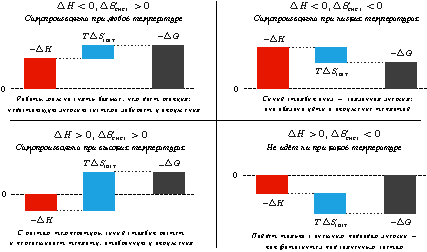
\includegraphics[width=\linewidth]{figs/gibbs_energy/gibbs_energy_budget.pdf}
    \caption{Связанная и полезная энергии в балансе реакции в зависимости от её типа.}
    \label{fig:gibbs_energy_budget}
\end{figure}

Может ли реакция протекать, если $\Delta G > 0$? Самопроизвольно~--- не может, но она будет происходить, если подводить к ней энергию извне. С точки зрения термодинамики это равносильно тому, что мы расширяем рассматриваемую систему, включая в неё источник внешней энергии. При этом окажется, что общая энтропия такой расширенной системы всё равно будет возрастать, то есть второй закон термодинамики будет соблюдаться.

Хорошим примером реакции с внешним подводом энергии является фотосинтез, в ходе которого растения превращают углекислый газ и воду в глюкозу и кислород:

\begin{equation*}
    \ce{6CO2 + 6H2O -> C6H12O6 + 6O2}, \qquad \Delta G^{\circ} = +\qty{2870}{\ruKJ\per\ruMole}.
\end{equation*}

Сама по себе эта реакция в обычных условиях идти не может. Наоборот, в живых организмах обычно протекает обратный процесс~--- окисление глюкозы, высвобождающее большое количество свободной энергии, которая затем тратится на работу в клетке (например, на биохимические реакции, которые несамопроизвольны и требуют подвода энергии). Но растения используют внешний подвод энергии, проводя синтез, поглощая солнечное излучение.

\subsection*{Куда расходуется энергия реакции}

Итак, мы разобрались, откуда в химических реакциях возникает новая энтропия. Теперь давайте проследим весь путь энергии по шагам на конкретном примере~--- уже знакомой нам реакции водорода с кислородом при \qty{298}{\ruK}, но на этот раз с образованием жидкой воды:

\reaction*{H2_{(\text{г})} + \frac{1}{2}O2_{(\text{г})} -> H2O_{(\text{ж})}}

Стандартные значения для неё:

\begin{equation*}
    \Delta H^{\circ} = \qty{-285,8}{\ruKJ\per\ruMole}, \qquad \Delta S^{\circ}_{\text{сист}} = \qty{-163,3}{\ruJ\per\ruK\ruMole}.
\end{equation*}

Нам понадобится ещё одна величина. Равенство $\Delta S_{\text{сист}} = Q/T$ справедливо для системы только в том случае, если процесс обратим. В общем случае баланс энтропии удобнее записать так:

\begin{equation}
    \label{eq:entropy_production}
    \Delta S_{\text{сист}} = \frac{Q_{\text{сист}}}{T} + \sigma, \qquad \sigma \geqslant 0,
\end{equation}

где $Q_{\text{сист}}$~--- теплота, полученная системой, а $\sigma$~--- \emph{произведённая} энтропия, то есть та самая новая энтропия. Для большого равновесного термостата производства энтропии нет, поэтому

\begin{equation*}
    \Delta S_{\text{окр}} = \frac{Q_{\text{окр}}}{T} = -\frac{Q_{\text{сист}}}{T}.
\end{equation*}

\textit{I этап. Исходное состояние.} У нас имеется \qty{1}{\ruMole} \ce{H2} и \qty{0,5}{\ruMole} \ce{O2}; сумма стандартных энтропий реагентов около \qty{233,3}{\ruJ\per\ruK\ruMole}. Имеющуюся энергию условно разделим на тепловую и химическую. Химическую часть грубо оценим по энергиям связей:

\begin{equation*}
    E_{\ce{H\bond{1}H}} + \frac{1}{2} E_{\ce{O\bond{2}O}} \approx \num{436} + \num{249} = \qty{685}{\ruKJ\per\ruMole}.
\end{equation*}

При \qty{298}{\ruK} это примерно $276\,kT$ в расчёте на одну образующуюся молекулу воды, или, что то же самое, $276\,RT$ на моль реакции.

\textit{II этап. Активация реакции.} Чтобы реакция началась, сталкивающиеся молекулы должны преодолеть энергетический барьер. Доля таких столкновений от общего числа определяется больцмановским множителем порядка $\exp(-E_a/RT)$, где $E_a$~--- мольная энергия активации. Образование комплекса из реагирующих частиц, предшествующего реакции, может сопровождаться локальным уменьшением энтропии, но это не нарушение второго начала термодинамики, которое не запрещает флуктуации (ведь полная энтропия системы и окружения при этом не уменьшается). Реальная реакция водорода с кислородом идёт по цепному механизму, но нам сейчас достаточно упрощённой картины.

\textit{III этап. Перестройка связей.} Разрыв старых связей требует \qty{685}{\ruKJ\per\ruMole}. Образование двух связей \ce{O-H} выделяет $2 \cdot \num{463} = \qty{926}{\ruKJ\per\ruMole}$. Итого выделяется примерно \qty{241}{\ruKJ\per\ruMole} (точнее~--- \num{241,8}).

Куда девается эта энергия? Кажется, что превращается в теплоту. Однако это не так. Сначала она оказывается во внутренних степенях свободы\footnote{Внутренние степени свободы~--- это все способы движения молекулы, кроме перемещения её как целого: колебания
атомов относительно друг друга, вращение молекулы и (при очень больших энергиях) возбуждение электронных оболочек. Каждая такая степень свободы~--- отдельное <<хранилище>>, в которое можно положить порцию энергии.} продуктов и в энергии их движения, причём не обязательно у одной молекулы.

Энтропия на этом шаге практически не произведена. Энергия просто переехала из одного концентрированного хранилища (химическая связь) в другое (колебания молекулы).

\textit{IV этап. Термализация.} Накачанные энергией молекулы \ce{H2O} сталкиваются с соседями порядка $10^{10}$ раз в секунду. При каждом столкновении часть колебательной энергии уходит партнёру как поступательная и вращательная. Крупные порции дробятся на кванты размером порядка $kT$ и расползаются по сотням молекул. Именно в этот момент энтропия увеличивается.

Если выделившаяся энергия \qty{241,8}{\ruKJ\per\ruMole} полностью уходит в окружение при \qty{298}{\ruK}, то на одну молекулу приходится

\begin{equation*}
    \frac{\num{241800}}{RT} = \frac{\num{241800}}{\num{2477,6}} \approx 98
\end{equation*}

условных тепловых квантов $kT$, а окружение получает энтропию

\begin{equation*}
    \Delta S_{\text{окр}} = \frac{\num{241800}}{\num{298}} \approx \qty{811,4}{\ruJ\per\ruK\ruMole}.
\end{equation*}

Начиная с этого момента термализованная энергия уже не может быть использована для совершения работы\footnote{Микроскопически динамика обратима, но информация о том, откуда пришла энергия, переехала в так называемые многочастичные корреляции, недоступные никакому макроскопическому рычагу.}.

\textit{V этап. Конденсация.} При конденсации пара в жидкость выделяется ещё \qty{44,0}{\ruKJ\per\ruMole}, которые тоже термализуются. Это ещё примерно

\begin{equation*}
    \frac{\num{44000}}{\num{2477,6}} \approx 18
\end{equation*}

тепловых квантов и

\begin{equation*}
    \frac{\num{44000}}{\num{298}} \approx \qty{147,7}{\ruJ\per\ruK\ruMole}
\end{equation*}

энтропии окружения. Система при этом продолжает терять энтропию (примерно \qty{118,9}{\ruJ\per\ruK\ruMole}). Обратите внимание, что средняя кинетическая энергия поступательного движения при той же температуре не становится меньше, потому что выделяющаяся теплота связана преимущественно с межмолекулярным взаимодействием.

Подведём итоги. Суммарный прирост энтропии окружения при полном переходе к жидкой воде:

\begin{equation*}
    \Delta S_{\text{окр}} \approx \num{811,4} + \num{147,7} \approx \qty{959,1}{\ruJ\per\ruK\ruMole},
\end{equation*}

или, в единицах $R$,

\begin{equation*}
    \frac{\num{959,1}}{\num{8,314}} \approx \num{115,3}.
\end{equation*}

Это значит, что в расчёте на одну образовавшуюся молекулу воды число доступных микросостояний окружения увеличивается примерно в $e^{115} \approx 10^{50}$ раз, а для моля реакций множитель равен $e^{115 N_A}$.

Система при этом теряет энтропию: $\Delta S_{\text{сист}} = \qty{-163,3}{\ruJ\per\ruK\ruMole}$. Подставим это значение в баланс~\eqref{eq:entropy_production}, помня, что система теплоту не получает, а отдаёт ($Q_{\text{сист}} = \Delta H < 0$):

\begin{equation*}
    \Delta S_{\text{сист}} = \sigma - \num{959,1}, \qquad \text{откуда} \qquad \sigma = -\num{163,3} + \num{959,1} \approx \qty{795,8}{\ruJ\per\ruK\ruMole}.
\end{equation*}

Полная энтропия, разумеется, возрастает ровно на эту же величину:

\begin{equation*}
    \Delta S_{\text{общ}} = -\num{163,3} + \num{959,1} \approx \qty{795,8}{\ruJ\per\ruK\ruMole}.
\end{equation*}

То же самое значение можно найти и через энергию Гиббса:

\begin{equation*}
    \Delta G = \Delta H - T \Delta S_{\text{сист}} = -\num{285,8} - \num{298} \cdot (-\num{0,1633}) \approx \qty{-237,1}{\ruKJ\per\ruMole}.
\end{equation*}

Величина $\left| \Delta G \right|$~--- это максимальная полезная работа. Если эта работа не снимается, то все \qty{237,1}{\ruKJ\per\ruMole} термализуются и производят энтропию

\begin{equation*}
    \frac{\num{237100}}{\num{298}} \approx \qty{795,6}{\ruJ\per\ruK\ruMole},
\end{equation*}

то есть то самое значение $\sigma$, которое мы нашли из баланса. А минимальная теплота, которая обязана уйти в окружение, чтобы компенсировать убыль энтропии в системе, равна

\begin{equation*}
    \left| T \Delta S_{\text{сист}} \right| \approx \qty{48,7}{\ruKJ\per\ruMole}.
\end{equation*}

Именно это и есть связанная энергия, то есть разница между \qty{285,8}{\ruKJ\per\ruMole}, которые реакция отдаёт, и \qty{237,1}{\ruKJ\per\ruMole}, которые она способна отдать в виде полезной работы.

Теперь давайте перейдём к решению последних задач этой главы. В этот раз они будет посложнее, сможете ли вы их решить?

\begin{termlist}
    \hyperref[term:thermalization]{Термализация},
    \hyperref[term:gibbs_energy]{энергия Гиббса},
    \hyperref[term:bound_energy]{связанная энергия}.
\end{termlist}

\begin{problem}{}{gibbs_energy1}
    \emph{Термитная смесь} содержит в себе порошки алюминия и оксида железа(III), в которых оксид железа выступает окислителем, а алюминий~--- топливом. Если поджечь такую смесь, то горение происходит с ослепительной вспышкой, а температура смеси становится настолько высокой, что термитной шашкой можно прожечь лист железа. Реакция горения протекает так:
    \reaction*{2Al_{(\text{тв})} + Fe2O3_{(\text{тв})} -> Al2O3_{(\text{тв})} + 2Fe_{(\text{тв})}{.}}

    \begin{enumerate}[label=\arabic*)]
        \item Рассчитайте $\Delta H^{\circ}$, $\Delta S^{\circ}_{\text{сист}}$ и $\Delta G^{\circ}$ этой реакции при \qty{298}{\ruK}.
        \item К какой строке таблицы~\ref{tab:gibbs_and_temperature} она относится и что это означает?
        \item Какую максимальную полезную работу способна дать реакция и какая часть выделяющейся энергии оказывается связанной?
    \end{enumerate}

    Данные. Стандартные теплоты образования $\Delta{}_fH^{\circ}$, \unit{\ruKJ\per\ruMole}: \ce{Fe2O3} \num{-824,2}, \ce{Al2O3} \num{-1675,7}. Стандартные энтропии $S^{\circ}$, \unit{\ruJ\per\ruK\ruMole}: \ce{Al} \num{28,3}, \ce{Fe2O3} \num{87,4}, \ce{Al2O3} \num{50,9}, \ce{Fe} \num{27,3}.
    \begin{sol}{\ref{prob:gibbs_energy1}}
        1)~Энтальпию и энтропию реакции рассчитываем по закону Гесса (теплоты образования простых веществ равны нулю):
        \begin{equation*}
            \Delta H^{\circ} = \num{-1675,7} - (\num{-824,2}) = \qty{-851,5}{\ruKJ\per\ruMole},
        \end{equation*}
        \begin{equation*}
            \Delta S^{\circ}_{\text{сист}} = (\num{50,9} + 2 \cdot \num{27,3}) - (2 \cdot \num{28,3} + \num{87,4}) = \num{105,5} - \num{144,0} = \qty{-38,5}{\ruJ\per\ruK\ruMole}.
        \end{equation*}
        По формуле~\eqref{eq:gibbs_criterion}
        \begin{equation*}
            \Delta G^{\circ} = \num{-851,5} - \num{298} \cdot (\num{-0,0385}) = \num{-851,5} + \num{11,5} = \qty{-840,0}{\ruKJ\per\ruMole}.
        \end{equation*}

        2)~$\Delta H < 0$ и $\Delta S_{\text{сист}} < 0$~--- такие знаки изменений соответствуют второй строке таблицы. Реакция самопроизвольна при низких температурах и должна <<выключаться>> при высоких. Формальная граница
        \begin{equation*}
            T = \frac{\Delta H}{\Delta S_{\text{сист}}} = \frac{\num{-851500}}{\num{-38,5}} \approx \qty{22100}{\ruK},
        \end{equation*}
        то есть в несколько раз выше температуры поверхности Солнца. Задолго до неё все участники перейдут в парообразное состояние, так что на практике эта реакция самопроизвольна всегда. Таким образом, строки таблицы~\ref{tab:gibbs_and_temperature} говорят лишь о том, в каком направлении находится граница, но ничего не говорят о том, достижима ли она.

        3)~Максимальная полезная работа~--- это $|\Delta G^{\circ}| = \qty{840,0}{\ruKJ\per\ruMole}$, а связанная энергия равна
        \begin{equation*}
            \left| T \Delta S_{\text{сист}} \right| = \qty{11,5}{\ruKJ\per\ruMole},
        \end{equation*}
        то есть всего \qty{1,3}{\percent} от выделяющейся энергии. Энтропийный налог очень мал, почти вся энергия реакции <<свободна>>. Однако в термите её никто не снимает в виде работы, потому что его назначение как раз в том, чтобы термализовать всю энергию и разогреться до \qty{2500}{\degreeCelsius}.
    \end{sol}
\end{problem}

\begin{problem}{}{gibbs_energy2}
    Запаянную трубку с \ce{NO2} (бурый газ) опускают в стакан со льдом, при этом окраска почти изчезает. Затем трубку извлекают и погружают в стакан с горячей водой, из-за чего газ в трубке становится ещё более бурым, чем изначально. Причина такого изменения окраски~--- это обратимая димеризация
    \reaction*{2NO2_{(\text{г})} <=> N2O4_{(\text{г})}{,}}
    в которой \ce{N2O4} бесцветен, а \ce{NO2} ярко-бурый.

    \begin{enumerate}[label=\arabic*)]
        \item Рассчитайте $\Delta H^{\circ}$, $\Delta S^{\circ}_{\text{сист}}$ и $\Delta G^{\circ}$ прямой реакции при \qty{298}{\ruK}.
        \item Найдите температуру, выше которой знак $\Delta G^{\circ}$ меняется.
        \item Объясните проведённый эксперимент.
    \end{enumerate}

    Данные. $\Delta{}_fH^{\circ}$, \unit{\ruKJ\per\ruMole}: \ce{NO2} \num{33,2}, \ce{N2O4} \num{9,2}. $S^{\circ}$, \unit{\ruJ\per\ruK\ruMole}: \ce{NO2} \num{240,1}, \ce{N2O4} \num{304,4}.
    \begin{sol}{\ref{prob:gibbs_energy2}}
        1)~По закону Гесса:
        \begin{equation*}
            \Delta H^{\circ} = \num{9,2} - 2 \cdot \num{33,2} = \qty{-57,2}{\ruKJ\per\ruMole},
        \end{equation*}
        \begin{equation*}
            \Delta S^{\circ}_{\text{сист}} = \num{304,4} - 2 \cdot \num{240,1} = \qty{-175,8}{\ruJ\per\ruK\ruMole}.
        \end{equation*}
        Знаки измерений энтальпии и энтропии предсказуемы, потому что образуется новая связь \ce{N-N}, а из двух молекул газа получается одна (энтропия падает). Тогда
        \begin{equation*}
            \Delta G^{\circ} = \num{-57,2} - \num{298} \cdot (\num{-0,1758}) = \num{-57,2} + \num{52,4} = \qty{-4,8}{\ruKJ\per\ruMole}.
        \end{equation*}
        Величина изменения энергии Гиббса в прямой реакции отрицательная, но очень маленькая, она всего вдвое больше $RT = \qty{2,5}{\ruKJ\per\ruMole}$. Энтальпийный и энтропийный члены почти уравновешивают друг друга.

        2)~Температура, соответствующая $\Delta G^{\circ} = 0$:
        \begin{equation*}
            T = \frac{\Delta H^{\circ}}{\Delta S^{\circ}_{\text{сист}}} = \frac{\num{-57200}}{\num{-175,8}} \approx \qty{325}{\ruK} \approx \qty{52}{\degreeCelsius}.
        \end{equation*}

        3)~Это тоже вторая строка таблицы~\ref{tab:gibbs_and_temperature}, но, в отличие от реакции горения термитной смеси из задачи~\ref{prob:gibbs_energy1}, граница здесь оказывается в бытовом диапазоне температур. Так получилось потому, что оба члена малы и сравнимы. Ниже \qty{52}{\degreeCelsius} самопроизвольна прямая реакция (димеризация)~--- смесь обесцвечивается. При нагреве самопроизвольной становится обратная реакция разложения димера~--- трубка буреет.
    \end{sol}
\end{problem}

\begin{problem}{}{gibbs_energy3}
    $\bigstar$ Метанол получают в промышленности из \emph{синтез-газа}:
    \reaction*{CO_{(\text{г})} + 2H2_{(\text{г})} -> CH3OH_{(\text{г})}{.}}
    Справочника под рукой у вас нет, но зато известны значения энергии Гиббса этой реакции при двух температурах: $\Delta G^{\circ}(\qty{298}{\ruK}) = \qty{-25,2}{\ruKJ\per\ruMole}$ и $\Delta G^{\circ}(\qty{400}{\ruK}) = \qty{-2,8}{\ruKJ\per\ruMole}$. Найдите $\Delta H^{\circ}$ и $\Delta S^{\circ}_{\text{сист}}$ реакции, а также температуру, выше которой она перестаёт быть самопроизвольной. Считайте, что $\Delta H$ и $\Delta S_{\text{сист}}$ от температуры не зависят. Промышленный синтез ведут при \qty{250}{\degreeCelsius}~--- как это согласуется с ответом?
    \begin{sol}{\ref{prob:gibbs_energy3}}
        Запись $\Delta G = \Delta H - T \Delta S_{\text{сист}}$~--- это уравнение прямой относительно $T$: свободный член равен $\Delta H$, а угловой коэффициент равен $-\Delta S_{\text{сист}}$. Двух точек достаточно, чтобы получить уравнение этой прямой, решив систему уравнений:
        \begin{equation*}
            \Delta S^{\circ}_{\text{сист}} = -\frac{\Delta G^{\circ}_2 - \Delta G^{\circ}_1}{T_2 - T_1} = -\frac{\num{-2,8} - (\num{-25,2})}{\num{400} - \num{298}} = -\frac{\num{22,4}}{\num{102}} = \qty{-219,6}{\ruJ\per\ruK\ruMole},
        \end{equation*}
        \begin{equation*}
            \Delta H^{\circ} = \Delta G^{\circ}_1 + T_1 \Delta S^{\circ}_{\text{сист}} = \num{-25,2} + \num{298} \cdot (\num{-0,2196}) = \qty{-90,6}{\ruKJ\per\ruMole}.
        \end{equation*}
        Реакция экзотермическая, а из трёх молей газа получается один, поэтому энтропия системы сильно падает.

        Граница самопроизвольности:
        \begin{equation*}
            T = \frac{\Delta H^{\circ}}{\Delta S^{\circ}_{\text{сист}}} = \frac{\num{-90600}}{\num{-219,6}} \approx \qty{413}{\ruK} \approx \qty{140}{\degreeCelsius}.
        \end{equation*}

        Получается, что при рабочих \qty{250}{\degreeCelsius} (\qty{523}{\ruK}) энергия Гиббса становится положительной:
        \begin{equation*}
            \Delta G^{\circ} = \num{-90,6} + \num{523} \cdot \num{0,2196} \approx +\qty{24,3}{\ruKJ\per\ruMole}.
        \end{equation*}
        Почему процесс ведут именно так? Во-первых, при \qty{140}{\degreeCelsius} реакция практически не идёт из-за низкой скорости, так как катализатор этой реакции начинает работать только горячим, и приходится жертвовать термодинамической выгодой ради кинетики. Во-вторых, не забывайте о том, что величина $\Delta G^{\circ}$ относится к \emph{стандартным} условиям, то есть к давлению \qty{1}{\ruAtm} для каждого газа. Промышленный процесс же ведут под давлением в 50--100 атмосфер, а сжатие смеси, в которой из трёх объёмов газа получается один, что сдвигает равновесие в сторону образования меньшего количества частиц в реакционной смеси. Подробнее о том, почему $\Delta G^{\circ} > 0$ не означает <<реакция запрещена>>, речь пойдёт в задаче~\ref{prob:gibbs_energy10}.
    \end{sol}
\end{problem}

\begin{problem}{}{gibbs_energy4}
    $\bigstar$ Природный газ можно сжечь в тепловой машине, снимая тепло, а можно окислить в топливном элементе, где та же реакция разделена на два электродных процесса и производит электрический ток:
    \reaction*{CH4_{(\text{г})} + 2O2_{(\text{г})} -> CO2_{(\text{г})} + 2H2O_{(\text{ж})}{.}}

    \begin{enumerate}[label=\arabic*)]
        \item Найдите максимальную полезную работу этой реакции при \qty{298}{\ruK} и долю связанной энергии.
        \item Сравните её с работой идеальной тепловой машины, получающей ту же теплоту при \qty{1200}{\ruK} и отдающей её холодильнику при \qty{300}{\ruK} (КПД цикла Карно $\eta = 1 - T_2/T_1$).
        \item Объясните, почему у топливного элемента предел выше.
    \end{enumerate}

    Данные. $\Delta{}_fH^{\circ}$, \unit{\ruKJ\per\ruMole}: \ce{CH4} \num{-74,6}, \ce{CO2} \num{-393,5}, \ce{H2O} (ж.) \num{-285,8}. $S^{\circ}$, \unit{\ruJ\per\ruK\ruMole}: \ce{CH4} \num{186,3}, \ce{O2} \num{205,2}, \ce{CO2} \num{213,8}, \ce{H2O} (ж.) \num{70,0}.
    \begin{sol}{\ref{prob:gibbs_energy4}}
        1)~Рассчитываем по закону Гесса:
        \begin{equation*}
            \Delta H^{\circ} = \num{-393,5} + 2 \cdot (\num{-285,8}) - (\num{-74,6}) = \qty{-890,5}{\ruKJ\per\ruMole},
        \end{equation*}
        \begin{equation*}
            \Delta S^{\circ}_{\text{сист}} = (\num{213,8} + 2 \cdot \num{70,0}) - (\num{186,3} + 2 \cdot \num{205,2}) = \qty{-242,9}{\ruJ\per\ruK\ruMole}.
        \end{equation*}
        Энтропия падает, потому что три моля газа превращаются в один моль газа и два моля жидкости. Отсюда
        \begin{equation*}
            \Delta G^{\circ} = \num{-890,5} + \num{298} \cdot \num{0,2429} = \num{-890,5} + \num{72,4} = \qty{-818,1}{\ruKJ\per\ruMole}.
        \end{equation*}
        Связанная энергия~--- \qty{72,4}{\ruKJ\per\ruMole}, то есть \qty{8,1}{\percent} от энергии реакции. Предельный КПД топливного элемента
        \begin{equation*}
            \frac{\num{818,1}}{\num{890,5}} \approx \num{0,919}, \text{ то есть } \qty{91,9}{\percent}.
        \end{equation*}

        2)~Для тепловой машины:
        \begin{equation*}
            \eta = 1 - \frac{\num{300}}{\num{1200}} = \num{0,75}, \qquad W = \num{0,75} \cdot \num{890,5} \approx \qty{668}{\ruKJ\per\ruMole},
        \end{equation*}
        то есть примерно на \qty{150}{\ruKJ\per\ruMole} меньше. Это оптимистичная оптимистичная оценка, потому что цикл Карно недостижим, реальные электростанции дают \num{40}--\qty{60}{\percent}.

        3)~Разница~--- в том, \emph{на каком этапе} платится энтропийный налог. Тепловая машина сначала \emph{термализует} всю энергию реакции, а термализованную энергию, как мы выяснили, уже нельзя полностью превратить в работу: чтобы вернуть рабочее тело в исходное состояние, машина обязана сбросить в холодильник теплоту, уносящую всю полученную энтропию. Размер этого налога задаётся отношением температур $T_2/T_1$ и никак не связан с $\Delta S_{\text{сист}}$ самой реакции.

        Топливный элемент энергию не термализует: электроны уходят во внешнюю цепь напрямую, минуя стадию термализации. Поэтому остаётся только энтропийный налог~--- та теплота $|T \Delta S_{\text{сист}}|$, которая компенсирует убыль энтропии самой реагирующей системы.
    \end{sol}
\end{problem}

\begin{problem}{}{gibbs_energy5}
    $\bigstar$ Давайте рассмотрим реакцию неполного сгорания угля:
    \reaction*{C_{(\text{графит})} + \frac{1}{2}O2_{(\text{г})} -> CO_{(\text{г})}{.}}

    \begin{enumerate}[label=\arabic*)]
        \item Рассчитайте $\Delta H^{\circ}$ и $\Delta G^{\circ}$ при \qty{298}{\ruK} и сравните их модули.
        \item Пусть эту реакцию удалось провести в идеальном топливном элементе и снять всю возможную работу. Откуда возьмётся энергия сверх выделившейся химической?
        \item Неужели у нас получается вечный двигатель второго рода~--- устройство, целиком превращающее теплоту окружения в работу?
    \end{enumerate}

    Данные. $\Delta{}_fH^{\circ}(\ce{CO}) = \qty{-110,5}{\ruKJ\per\ruMole}$. $S^{\circ}$, \unit{\ruJ\per\ruK\ruMole}: \ce{C} (графит) \num{5,7}, \ce{O2} \num{205,2}, \ce{CO} \num{197,7}.
    \begin{sol}{\ref{prob:gibbs_energy5}}
        1)~Тепловой эффект реакции здесь~--- это теплота образования \ce{CO}, то есть \qty{-110,5}{\ruKJ\per\ruMole}. Рассчитываем энтропию:
        \begin{equation*}
            \Delta S^{\circ}_{\text{сист}} = \num{197,7} - \num{5,7} - \frac{1}{2} \cdot \num{205,2} = +\qty{89,4}{\ruJ\per\ruK\ruMole}
        \end{equation*}
        (количество вещества газа в системе увеличивается, твёрдый углерод переносится в газовую фазу). Значит,
        \begin{equation*}
            \Delta G^{\circ} = \num{-110,5} - \num{298} \cdot \num{0,0894} = \num{-110,5} - \num{26,6} = \qty{-137,1}{\ruKJ\per\ruMole}.
        \end{equation*}
        $|\Delta G^{\circ}| = \num{137,1} > |\Delta H^{\circ}| = \num{110,5}$, то есть реакция способна дать работы больше, чем выделяет химической энергии.

        2)~Недостающие \qty{26,6}{\ruKJ\per\ruMole} система забирает у окружения в виде теплоты. Если энтропия системы растёт, то <<налог>> оказывается отрицательным и вместо того чтобы сбрасывать теплоту, система \emph{поглощает} её. Проверим баланс энтропии. Система получает $Q_{\text{сист}} = +\qty{26,6}{\ruKJ\per\ruMole}$, значит окружение теряет
        \begin{equation*}
            \Delta S_{\text{окр}} = -\frac{\num{26600}}{\num{298}} = \qty{-89,3}{\ruJ\per\ruK\ruMole},
        \end{equation*}
        а система, как мы рассчитали ранее, приобретает $+\qty{89,4}{\ruJ\per\ruK\ruMole}$. Суммарный эффект получается нулевой, что соответствует обратимому процессу для снятия максимального количества работы ($\sigma = 0$). Такой идеальный топливный элемент будет слегка \emph{охлаждать} сам себя.

        3)~Второй закон запрещает полное превращение теплоты в работу не вообще, а в \emph{циклическом} процессе~--- когда устройство после каждого цикла возвращается в исходное состояние. Здесь такого не происходит, потому что углерод расходуется безвозвратно. Возможность забрать теплоту у окружения имеется только из-за роста собственной энтропии системы, а этот ресурс не бесконечен: он закончится когда будет ихрасходован весь углерод.
    \end{sol}
\end{problem}

\begin{problem}{}{gibbs_energy6}
    $\bigstar$ Для реакции фотосинтеза
    \reaction*{6CO2 + 6H2O -> C6H12O6 + 6O2}
    в тексте раздела приведено значение $\Delta G^{\circ} = +\qty{2870}{\ruKJ\per\ruMole}$. Растение компенсирует эту энергию квантами света, причём хлорофилл наиболее эффективно поглощает красный свет с длиной волны около \qty{680}{\ruNm}.

    \begin{enumerate}[label=\arabic*)]
        \item Какова энергия 1~моля таких квантов?
        \item Каково минимальное число квантов, необходимое для синтеза одной молекулы глюкозы?
        \item В реальности фотосинтез расходует около \num{8} квантов на каждую выделившуюся молекулу \ce{O2}. Какова эффективность запасания энергии и куда девается остальное?
    \end{enumerate}

    Данные. Постоянная Планка $h = \qty{6,626e-34}{\ruJ\ruS}$, скорость света $c = \qty{3,00e8}{\ruM\per\ruS}$, постоянная Авогадро $N_A = \num{6,02e23}$.
    \begin{sol}{\ref{prob:gibbs_energy6}}
        1)~Энергия одного кванта равна:
        \begin{equation*}
            E = \frac{hc}{\lambda} = \frac{\num{6,626e-34} \cdot \num{3,00e8}}{\num{680e-9}} \approx \qty{2,92e-19}{\ruJ},
        \end{equation*}
        а на моль квантов
        \begin{equation*}
            E_m = E \cdot N_A = \num{2,92e-19} \cdot \num{6,02e23} \approx \qty{176}{\ruKJ\per\ruMole}.
        \end{equation*}
        Для сравнения, при \qty{298}{\ruK} это примерно $71\,RT$, то есть один такой квант несёт в семьдесят раз больше энергии, чем средний тепловой квант. Именно поэтому излучение так эффективно в проведении реакций с положительным значением энергии Гиббса, а простое нагревание~--- нет.

        2)~Минимальное количество необходимых квантов:
        \begin{equation*}
            n_{\min} = \frac{\num{2870}}{\num{176}} \approx \num{16,3}.
        \end{equation*}

        3)~В реальности уходит $8 \cdot 6 = \num{48}$ квантов, что даёт
        \begin{equation*}
            \num{48} \cdot \num{176} \approx \qty{8450}{\ruKJ\per\ruMole},
        \end{equation*}
        а запасается из них только \qty{2870}{\ruKJ\per\ruMole}:
        \begin{equation*}
            \frac{\num{2870}}{\num{8450}} \approx \num{0,34}, \text{ то есть около } \qty{34}{\percent}.
        \end{equation*}

        Оставшиеся две трети термализуются. Энергия кванта передаётся по цепочке молекул-переносчиков, и на каждой ступени часть её рассеивается. Такую цену приходится заплатить за то, чтобы процесс шёл в нужную сторону с адекватной скоростью, ведь полностью обратимый перенос энергии был бы бесконечно медленным.

        Заметим, что \qty{34}{\percent}~--- это эффективность использования уже поглощённых квантов. Если брать в расчёт всю солнечную энергию, падающую на лист, то у большинства растений реальный КПД примерно \num{1}--\qty{2}{\percent}, так как большая часть спектра вообще не поглощается хлорофиллом, а часть запасённой глюкозы растение тут же тратит на собственное дыхание.
    \end{sol}
\end{problem}

\begin{problem}{}{gibbs_energy7}
    $\bigstar$ Профессор Недоумелкин в панике. А всё потому, что он заглянул в справочник и обнаружил, что для превращения
    \reaction*{C_{(\text{алмаз})} -> C_{(\text{графит})}}
    энергия Гиббса отрицательна! <<Это что же получается, значит, алмаз в кольце моей жены прямо сейчас превращается в графит! Надо срочно сдать его в ломбард!>>~--- воскликнул он.

    Проверьте расчётом знак $\Delta G^{\circ}$ при \qty{298}{\ruK}, определите строку таблицы~\ref{tab:gibbs_and_temperature} и объясните, стоит ли профессору беспокоиться.

    Данные. $\Delta{}_fH^{\circ}(\ce{C}, \text{алмаз}) = +\qty{1,9}{\ruKJ\per\ruMole}$. $S^{\circ}$, \unit{\ruJ\per\ruK\ruMole}: алмаз \num{2,4}, графит \num{5,7}.
    \begin{sol}{\ref{prob:gibbs_energy7}}
        Графит~--- простое вещество, которое находится в стандартном состоянии, поэтому его теплота образования равна нулю, а алмаз~--- аллотропная модификация, и для него справочник даёт теплоту образования \qty{1,9}{\ruKJ\per\ruMole}. Тогда
        \begin{equation*}
            \Delta H^{\circ} = 0 - \num{1,9} = \qty{-1,9}{\ruKJ\per\ruMole},
        \end{equation*}
        \begin{equation*}
            \Delta S^{\circ}_{\text{сист}} = \num{5,7} - \num{2,4} = +\qty{3,3}{\ruJ\per\ruK\ruMole},
        \end{equation*}
        \begin{equation*}
            \Delta G^{\circ} = \num{-1,9} - \num{298} \cdot \num{0,0033} = \num{-1,9} - \num{1,0} = \qty{-2,9}{\ruKJ\per\ruMole}.
        \end{equation*}
        Это соответствует первой строке таблицы~\ref{tab:gibbs_and_temperature}, когда оба вклада отрицательны. Значит, превращение самопроизвольно при любой температуре. Получается, что с точки зрения термодинамики профессор то прав: алмаз при обычных условиях~--- не устойчивая форма углерода, а \emph{метастабильная}, а графит более устойчив.

        Впрочем, беспокоиться не о чем, потому что знак $\Delta G$ отвечает только на вопрос <<может ли в принципе протекать эта реакция?>>. Будет ли она происходить за разумное время, термодинамика ответить не может. Чтобы атом углерода перешёл из тетраэдрического окружения алмаза в слоистую решётку графита, нужно разорвать очень прочные ковалентные связи \ce{C-C}, для чего требуется очень высокая энергия активации~--- сотни килоджоулей на моль. Если принять $E_a \approx \qty{600}{\ruKJ\per\ruMole}$, то доля частиц, способных её преодолеть, имеет порядок
        \begin{equation*}
            e^{-E_a/RT} = e^{-\num{600000}/\num{2477,6}} = e^{-\num{242}} \approx 10^{-105}.
        \end{equation*}
        Поэтому за всё время существования текущей Вселенной с алмазом в кольце не произойдёт ничего страшного. Заметный переход начинается только при \num{1500}--\qty{1900}{\degreeCelsius} без доступа кислорода (в присутствии кислорода алмаз просто сгорит).
    \end{sol}
\end{problem}

\begin{problem}{}{gibbs_energy8}
    $\bigstar$ Реакцию, рассмотренную в текущем разделе:
    \reaction*{H2_{(\text{г})} + \frac{1}{2}O2_{(\text{г})} -> H2O_{(\text{ж})} {,}}
    ($\Delta H^{\circ} = \qty{-285,8}{\ruKJ\per\ruMole}$, $\Delta S^{\circ}_{\text{сист}} = \qty{-163,3}{\ruJ\per\ruK\ruMole}$, $\Delta G^{\circ} = \qty{-237,1}{\ruKJ\per\ruMole}$) можно осуществить тремя способами при \qty{298}{\ruK}:

    \begin{enumerate}[label=\arabic*)]
        \item сжечь в калориметре, не снимая никакой полезной работы;
        \item пропустить через топливный элемент, сняв \qty{80}{\percent} максимальной работы;
        \item провести обратимо, сняв всю максимальную работу.
    \end{enumerate}

    Для каждого случая найдите теплоту, полученную окружением, изменение его энтропии и произведённую энтропию $\sigma$ по балансу~\eqref{eq:entropy_production}. Объясните, почему $\sigma$ получается разной, хотя $\Delta H$, $\Delta S_{\text{сист}}$ и $\Delta G$~--- функции состояния и от способа проведения не зависят.
    \begin{sol}{\ref{prob:gibbs_energy8}}
        Алгоритм решения одинаков для всех трёх слачаев. При постоянном давлении энергетический баланс выглядит так:
        \begin{equation*}
            Q_{\text{сист}} = \Delta H + W,
        \end{equation*}
        где $W$~--- снятая с системы полезная (нерасширительная) работа. Дальше проводим расчёты, учитывая что $Q_{\text{окр}} = -Q_{\text{сист}}$, $\Delta S_{\text{окр}} = Q_{\text{окр}}/T$, а произведённая энтропия равна полному изменению энтропии: $\sigma = \Delta S_{\text{сист}} + \Delta S_{\text{окр}}$.

        1)~$W = 0$, поэтому $Q_{\text{сист}} = \Delta H = \qty{-285,8}{\ruKJ\per\ruMole}$, вся энергия уходит в окружение:
        \begin{equation*}
            \Delta S_{\text{окр}} = \frac{\num{285800}}{\num{298}} = \qty{959,1}{\ruJ\per\ruK\ruMole},
        \end{equation*}
        \begin{equation*}
            \sigma = \num{-163,3} + \num{959,1} = \qty{795,8}{\ruJ\per\ruK\ruMole}.
        \end{equation*}
        Этот случай и разобран подробно в разделе, вся свободная энергия термализовалась ($\sigma = |\Delta G|/T$).

        2)~$W = \num{0,8} \cdot \num{237,1} = \qty{189,7}{\ruKJ\per\ruMole}$, значит
        \begin{equation*}
            Q_{\text{сист}} = \num{-285,8} + \num{189,7} = \qty{-96,1}{\ruKJ\per\ruMole},
        \end{equation*}
        \begin{equation*}
            \Delta S_{\text{окр}} = \frac{\num{96100}}{\num{298}} = \qty{322,5}{\ruJ\per\ruK\ruMole},
        \end{equation*}
        \begin{equation*}
            \sigma = \num{-163,3} + \num{322,5} = \qty{159,2}{\ruJ\per\ruK\ruMole}.
        \end{equation*}
        Тот же ответ можно получить и быстрее, если сразу считать, какая часть свободной энергии не была снята и потому термализовалась:
        \begin{equation*}
            \sigma = \frac{|\Delta G| - W}{T} = \frac{\num{237100} - \num{189700}}{\num{298}} = \qty{159,1}{\ruJ\per\ruK\ruMole}.
        \end{equation*}

        3)~$W = \qty{237,1}{\ruKJ\per\ruMole}$, тогда
        \begin{equation*}
            Q_{\text{сист}} = \num{-285,8} + \num{237,1} = \qty{-48,7}{\ruKJ\per\ruMole},
        \end{equation*}
        \begin{equation*}
            \Delta S_{\text{окр}} = \frac{\num{48700}}{\num{298}} = \qty{163,4}{\ruJ\per\ruK\ruMole},
        \end{equation*}
        \begin{equation*}
            \sigma = \num{-163,3} + \num{163,4} \approx 0.
        \end{equation*}
        Обратите внимание, что \qty{48,7}{\ruKJ\per\ruMole}~--- это связанная энергия $|T \Delta S_{\text{сист}}|$, то есть та минимальная теплота, которую система обязана отдать окружению, чтобы возместить убыль собственной энтропии. Меньше отдать нельзя, и именно поэтому работы больше чем \qty{237,1}{\ruKJ\per\ruMole} снять невозможно.

        Почему $\sigma$ разная? Потому что $\sigma$~--- \emph{функция не состояния, а процесса}. $\Delta S_{\text{сист}} = \qty{-163,3}{\ruJ\per\ruK\ruMole}$ действительно одно и то же во всех трёх случаях. Но баланс~\eqref{eq:entropy_production} распределяет эту величину между двумя слагаемыми~--- полученной теплотой $Q_{\text{сист}}/T$ и произведённой энтропией $\sigma$,~--- и вот это распределение уже зависит от способа. Чем больше работы мы снимаем, тем меньше энергии термализуется и тем меньше новой энтропии производится. В идеале $\sigma = 0$, когда обратимый процесс не производит энтропии вообще, однако по этой же причине он идёт бесконечно медленно.
    \end{sol}
\end{problem}

\begin{problem}{}{gibbs_energy9}
    $\bigstar$ Первая стадия процесса усвоения глюкозы в клетке~--- это присоединение к ней фосфатной группы:
    \begin{equation*}
        \text{глюкоза} + \text{фосфат} \longrightarrow \text{глюкозо-6-фосфат} + \ce{H2O}, \qquad \Delta G^{\circ} = +\qty{13,8}{\ruKJ\per\ruMole}.
    \end{equation*}
    Одновременно в клетке идёт гидролиз аденозинтрифосфата (АТФ):
    \begin{equation*}
        \text{АТФ} + \ce{H2O} \longrightarrow \text{АДФ} + \text{фосфат}, \qquad \Delta G^{\circ} = \qty{-30,5}{\ruKJ\per\ruMole}.
    \end{equation*}

    \begin{enumerate}[label=\arabic*)]
        \item Почему первая реакция не идёт сама по себе?
        \item Покажите, что вместе эти две реакции идти могут.
        \item На каком основании энергии Гиббса двух реакций можно складывать?
        \item Достаточно ли просто смешать в пробирке глюкозу, фосфат и АТФ, чтобы получить глюкозо-6-фосфат?
        \item Сколько энтропии производит клетка на каждом таком акте при температуре тела \qty{310}{\ruK}?
    \end{enumerate}
    \begin{sol}{\ref{prob:gibbs_energy9}}
        1)~$\Delta G^{\circ} > 0$~--- значит, самопроизвольно это реакция идти не может. Как и в случае фотосинтеза, ей нужен внешний источник энергии.

        2)~Складываем уравнения (фосфат и вода при этом сокращаются):
        \begin{equation*}
            \text{глюкоза} + \text{АТФ} \longrightarrow \text{глюкозо-6-фосфат} + \text{АДФ},
        \end{equation*}
        \begin{equation*}
            \Delta G^{\circ} = \num{13,8} + (\num{-30,5}) = \qty{-16,7}{\ruKJ\per\ruMole} < 0.
        \end{equation*}
        Суммарный процесс оказывается самопроизволен. Такое объединение называют \emph{сопряжением} реакций: <<богатая>> реакция оплачивает <<бедную>>.

        3)~Потому что энергия Гиббса~--- это функция состояния.

        4)~Нет, закон Гесса позволяет \emph{считать} $\Delta G$ по любому воображаемому пути, но не обещает, что этот путь возможен на практике. Если просто смешать всё в пробирке, АТФ будет медленно гидролизоваться сам по себе, отдавая свои \qty{30,5}{\ruKJ\per\ruMole} на термализацию, а глюкоза так и останется нефосфорилированной. Каждая реакция пойдёт своим путём, и отрицательное $\Delta G$ одной из них никак не <<подталкивает>> другую.

        Чтобы сопряжение действительно работало, у двух реакций должен быть \emph{общий механизм}. В клетке это осуществляется при помощи фермента гексокиназа, который связывает обе молекулы в одном активном центре и переносит фосфатную группу непосредственно с АТФ на глюкозу, при этом свободный фосфат вообще не образуется. Другими словами, на практике отдельного шага с $\Delta G > 0$ просто нет. Есть единый процесс с $\Delta G = \qty{-16,7}{\ruKJ\per\ruMole}$.

        5)~Из \qty{30,5}{\ruKJ\per\ruMole}, которые отдал АТФ, \qty{13,8}{\ruKJ\per\ruMole} запасено в новой связи, а остальные \qty{16,7}{\ruKJ\per\ruMole} термализовались:
        \begin{equation*}
            \sigma = \frac{\num{16700}}{\num{310}} \approx \qty{53,9}{\ruJ\per\ruK\ruMole}.
        \end{equation*}
        Это расплата за то, что реакция идёт в нужную сторону: больше половины затраченной энергии термализуется, но без неё $\Delta G$ суммарного процесса не был бы отрицательным.
    \end{sol}
\end{problem}

\begin{problem}{}{gibbs_energy10}
    $\bigstar$ Сравните две реакции, для которых $\Delta G^{\circ} > 0$ при \qty{298}{\ruK}:
    \begin{equation*}
        \ce{N2O4_{(\text{г})} -> 2NO2_{(\text{г})}}, \qquad \Delta G^{\circ} = +\qty{4,8}{\ruKJ\per\ruMole},
    \end{equation*}
    \begin{equation*}
        \ce{2H2O_{(\text{ж})} -> 2H2_{(\text{г})} + O2_{(\text{г})}}, \qquad \Delta G^{\circ} = +\qty{474,2}{\ruKJ\per\ruMole}.
    \end{equation*}
    Согласно критерию~\eqref{eq:gibbs_criterion} самопроизвольно не может идти ни та, ни другая. Однако вода действительно не разлагается в обычных условиях, а вот запаянная трубка с \ce{N2O4} при комнатной температуре заметно бурая, то есть \ce{NO2} в ней есть. Нет ли здесь противоречия?
    \begin{sol}{\ref{prob:gibbs_energy10}}
        Дело в том, что мы сравнимаев стандартное состояние, для которого указаны значения $\Delta G^{\circ}$, и реальные процессы. \emph{Стандартное состояние} в данном случае в первую очередь означает, что каждый газ находится под давлением \qty{1}{\ruAtm} по отдельности. Величина $\Delta G^{\circ}$ отвечает на вопрос: <<в какую сторону пойдёт процесс, если и \ce{N2O4}, и \ce{NO2} находятся под давлением в одну атмосферу?>>. Ответ~--- в сторону \ce{N2O4}. Но это не то же самое, что <<\ce{NO2} в трубке не будет вовсе>>.

        Как только в трубке появляется хоть немного \ce{NO2}, его парциальное давление уже не равно \qty{1}{\ruAtm}, а вместе с составом смеси меняется и реальное $\Delta G$ (не $\Delta G^{\circ}$). Распад идёт до тех пор, пока $\Delta G$ не обратится в ноль~--- то есть до состояния \emph{химического равновесия}, то есть до определённого соотношения обоих веществ.

        Насколько далеко зайдёт распад, определяет $\Delta G^{\circ}$ в сравнении с тепловым масштабом $RT = \qty{2,5}{\ruKJ\per\ruMole}$:
        \begin{itemize}
            \item для \ce{N2O4} имеем $\num{4,8}/\num{2,5} \approx \num{1,9}$, всего около двух $RT$. Тепловое движение легко перевешивает такую разницу, и в равновесии присутствуют оба вещества в сопоставимых количествах~--- отсюда и бурый цвет;
            \item для воды $\num{474,2}/\num{2,5} \approx \num{191}$. Здесь разница огромна, равновесная доля продуктов имеет порядок $e^{-191} \approx 10^{-83}$, то есть в стакане воды не найдётся и одной молекулы водорода.
        \end{itemize}

        В целом запомните, что критерий $\Delta G < 0$ говорит о \emph{направлении} изменения из данного состояния, а не о том, что реакция запрещена. А $\Delta G^{\circ}$~--- это значение для одного конкретного, стандартного состояния. Чем оно больше по модулю, тем дальше от середины лежит равновесие. Количественную связь между $\Delta G^{\circ}$ и составом равновесной смеси мы разберём при изучении химических равновесий.
    \end{sol}
\end{problem}

\begin{problem}{}{gibbs_energy11}
    $\bigstar$ Живой организм строит из простых молекул очень сложные упорядоченные структуры, то есть локально сильно \emph{уменьшает} энтропию. Однако для этого ему нужна энергия. Взрослый человек потребляет с пищей около \qty{10000}{\ruKJ} в сутки, а температура тела \qty{310}{\ruK}.

    \begin{enumerate}[label=\arabic*)]
        \item Сколько энтропии человек производит за сутки?
        \item Во сколько раз при этом увеличивается статистический вес окружения? Постоянная Больцмана $k = \qty{1,380649e-23}{\ruJ\per\ruK}$.
        \item За сутки в организме обновляется около \qty{300}{\ruG} белка. Примите, что образование одной пептидной связи понижает энтропию примерно на \qty{200}{\ruJ\per\ruK\ruMole}, а средняя молярная масса аминокислотного остатка равна \qty{110}{\ruG\per\ruMole}. Сравните эту убыль с результатом первого пункта.
    \end{enumerate}
    \begin{sol}{\ref{prob:gibbs_energy11}}
        1)~Состав тела взрослого человека в среднем не меняется: сколько построено, столько и разрушено. Значит, вся энергия пищи в итоге термализуется и уходит в окружение в виде теплоты. Тогда
        \begin{equation*}
            \sigma = \frac{\num{1,0e7}}{\num{310}} \approx \num{3,2e4} \, \unit{\ruJ\per\ruK} = \qty{32}{\ruKJ\per\ruK}
        \end{equation*}
        за сутки.

        2)~Рассчитываем так же, как в задаче~\ref{prob:entropy_in_chemical_reactions6}, по формуле Больцмана:
        \begin{equation*}
            \ln \frac{\Omega_2}{\Omega_1} = \frac{\Delta S}{k} = \frac{\num{3,2e4}}{\num{1,380649e-23}} \approx \num{2,3e27},
        \end{equation*}
        \begin{equation*}
            \frac{\Omega_2}{\Omega_1} \approx e^{\num{2,3e27}} \approx 10^{\num{1,0e27}}.
        \end{equation*}

        3)~Количество аминокислотных остатков:
        \begin{equation*}
            n = \frac{\num{300}}{\num{110}} \approx \qty{2,7}{\ruMole},
        \end{equation*}
        столько же примерно образуется и пептидных связей. Убыль энтропии:
        \begin{equation*}
            \left| \Delta S \right| \approx \num{2,7} \cdot \num{200} \approx \qty{550}{\ruJ\per\ruK} = \qty{0,55}{\ruKJ\per\ruK},
        \end{equation*}
        то есть примерно \qty{1,7}{\percent} от произведённой энтропии~--- почти в 60 раз меньше.

        Отсюда видно, как в живых организмах локальное упорядочение оплачено производством энтропии с колоссальной переплатой. Организм это своего рода \emph{проточная} система, сквозь которую непрерывно течёт поток энергии, поступающей в концентрированном виде (пища) и уходящей в рассеянном (теплота и продукты обмена). Низкая энтропия в живых организмах держится до тех пор, пока этот поток идёт, но стоит ему прекратиться и структура распадается сама, потому что $\Delta G$ такого распада отрицателен.

        Заметим, справедливости ради, что оценка третьего пункта весьма груба. Значение \qty{200}{\ruJ\per\ruK\ruMole} условно, и упорядоченность организма не сводится к пептидным связям. Но нам важен здесь не точный ответ, а порядок величины, который отличается на два порядка, и никакое уточнение исходных цифр этого вывода не изменит.
    \end{sol}
\end{problem}

\clearpage